\section{Soot yield and morphology during methane pyrolysis in shock-tubes}

In this section, we focus on simulation of soot formation in shock-tubes using the constant volume reactor of omnisoot in order to (i) assess the performance of reaction mechanisms in prediction of the species mole fraction measured by laser diagnostics, and (ii) evaluate the accuracy of inception models to predict soot yield and morphology. 

Temperature ranges achieved in shock-tube experiments ($T>$2000~K) are relevant for plasma pyrolysis of methane (CH4) as an emerging alternative production method for co-generation of CB and hydrogen~\citep{fulcheri2023energy}. Achieving specific grades of CB for different target applications requires a good control over its properties such as its morphology (quantified by primary particle, $d_p$ and mobility diameter, $d_m$), composition (elemental carbon to hydrogen ratio), specific surface area (inversely proportional to $d_p$, $\mathrm{SSA}=6/(\rho_{soot}d_p)$) and internal nanostructure (composed of aligned graphitic shell and disordered core). However, this is challenging because of the complexity of soot inception and mass growth processes and its coupling with gas phase chemistry, dependence on local temperature and pressure, and short time scales of soot inception and surface growth~\citep{violi2005relative}. Therefore, robust particle dynamics models coupled with detailed chemical mechanisms are essential to better understand methane-to-CB conversion process under different feedstock compositions, and temperature and pressure time-histories.

While methane combustion has been extensively studied~\citep{wang2013pah} due to the need for a detailed chemical description of natural gas combustion, the formation of carbonaceous particles such as soot and CB from methane pyrolysis are not well understood yet. Significant differences exist between reaction mechanisms in prediction of $\mathrm{CH_4}$ and intermediate species such as $\mathrm{C_2H_2}$, and $\mathrm{C_2H_4}$ in flame and reactors~\citep{wang2013pah}. These uncertainties are amplified for larger hydrocarbons, especially polycyclic aromatic hydrocarbons (PAH) due to multiplicity of pathways that are not identified in available reaction mechanisms.

Shock tubes can be effective for kinetic studies and measurements of methane pyrolysis and the subsequent soot inception and surface growth due to the uniform and instant heating of the mixture behind the reflected shock to the desired temperature and pressure as well as the absence of complicating factors such as diffusion and mixing. The shock-wave propagation and reflection creates nearly isothermal and isobaric conditions ideal for kinetic studies of pyrolysis and particle formation. However, these conditions are limited to short residence times usually 1-3 ms, so they can only be used to study early stages of soot formation such as inception and surface growth, and not for processes occurring at longer residence times such as coagulation, graphitization and carbonization.

\begin{figure}[!htbp]
	\centering
	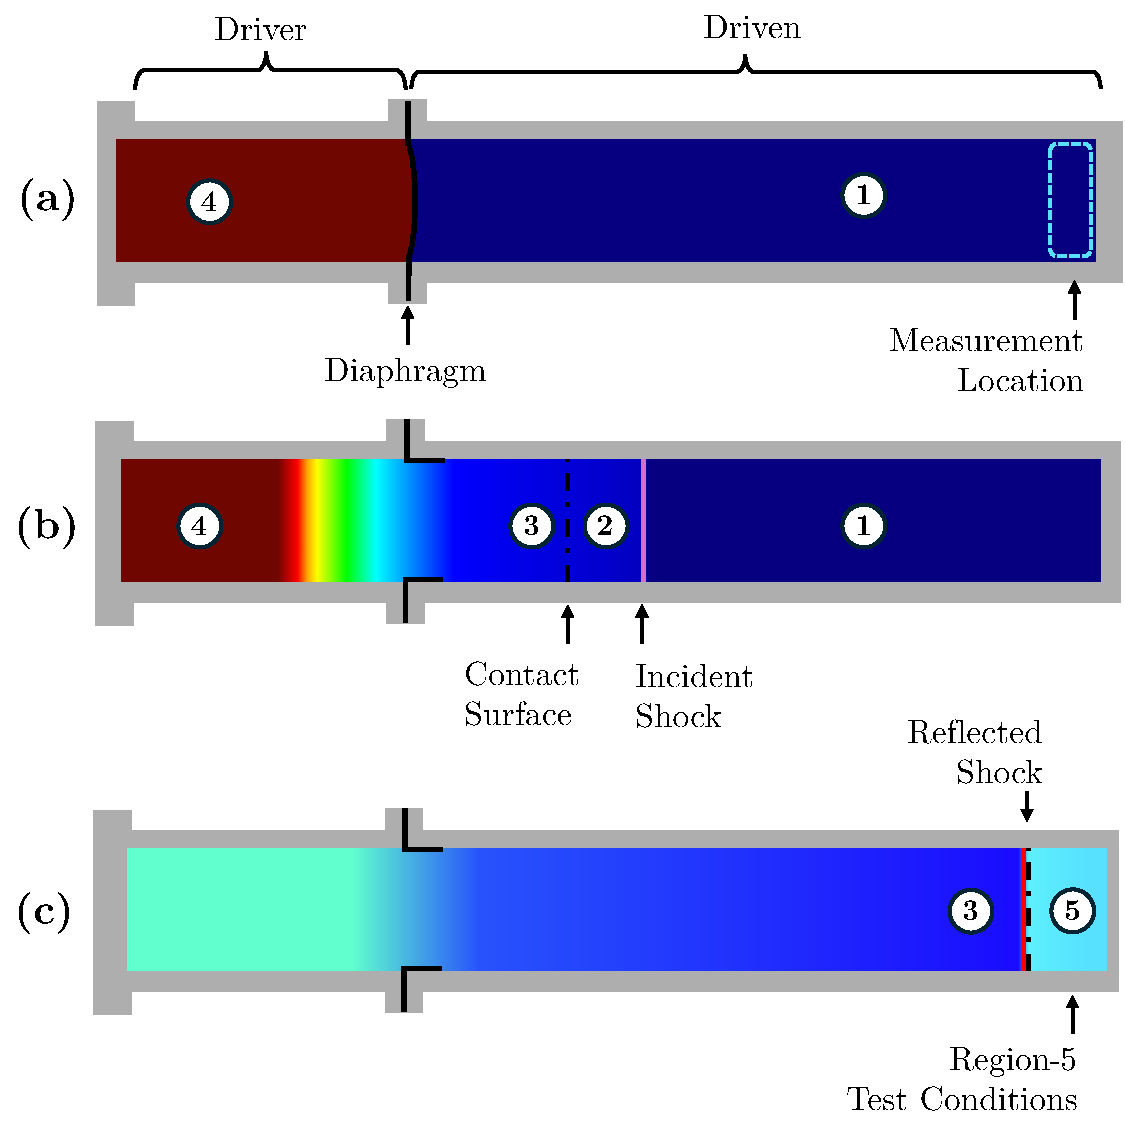
\includegraphics[height=80mm, ]{Figures/Results/Shocktube/shockwavestages.pdf}
	\caption{Different stages of shock wave propagation during shock-tube test from (a) before rupture of diaphragm leading to (b) propagation of incident shock towards the end of shock-tube and (c) its reflection from the end wall that increases pressure and temperature of test gas (Reprinted from Ref.~\citep{HansonGroupShockTube}}
	\label{fig:shockwave}
\end{figure}

Different stages of shock-wave propagation is illustrated in Fig.\ref{fig:shockwave}. A shock tube consists of a driver and a driven section separated by a single-use diaphragm. The driver section contains usually an inert gas with a low molecular weight such as He, and the driven section is filled with the studied test gas. The driver section is pressurized to the desired pressure until the rupture of the diaphragm. This creates a shock wave that propagates through the driven section causing a pressure and temperature jump in the test gas. 

After reaching the end wall, the shock wave reflects back towards the driver end of the shock-tube resulting in a secondary compression and heating of the mixture, and ultimately stagnating the test gas. In nearly 10 $\mathrm{\mu}$s, this shock-heating process can bring the test gas from room-temperature to temperatures upwards of 10,000 K, and pressures more than 1000 atm.



%Figure~\ref{fig:shocktubeschem} (left pane) illustrates the schematics of a shock-tube along with the idealized wave diagram. Shock-tubes are typically designed as a several meter long cylindrical tube separated by thin diaphragm into a smaller driver section filled a high pressure inert gas, and a longer driven section with diluted reactants. When the diaphragm is ruptured, the first shock wave propagates through the reactant mixture. The front shock compresses the reactants adiabatically raising the temperature and pressure throughout the shock-tube from $\mathrm{T_1}$, $\mathrm{P_1}$ to $\mathrm{T_2}$, $\mathrm{P_2}$. The passage of the reflected shock from the end wall heats up the reactants for the second time reaching $\mathrm{T_5}$, $\mathrm{P_5}$. Figure~\ref{fig:shocktubeschem} (right pane) shows the first and second jump in pressure due to the front and reflected shocks, respectively, and the variation in soot volume fraction during the pyrolysis of 0.03\% benzene in Ar. The reflected shock creates a nearly still mixture with a constant temperature and pressure (as shown in left pane of Figure~\ref{fig:shocktubeschem}) which provides an ideal condition for kinetic studies and rate constant investigations~\citep{kee2017chemically}. Therefore, the use of a shock tube provides a unique opportunity for investigating the kinetics of soot formation from fuels and at various temperatures, pressures and concentrations.

%\begin{figure}[!htbp]
%	\centering
%	\begin{subfigure}[t]{0.4\textwidth}
%		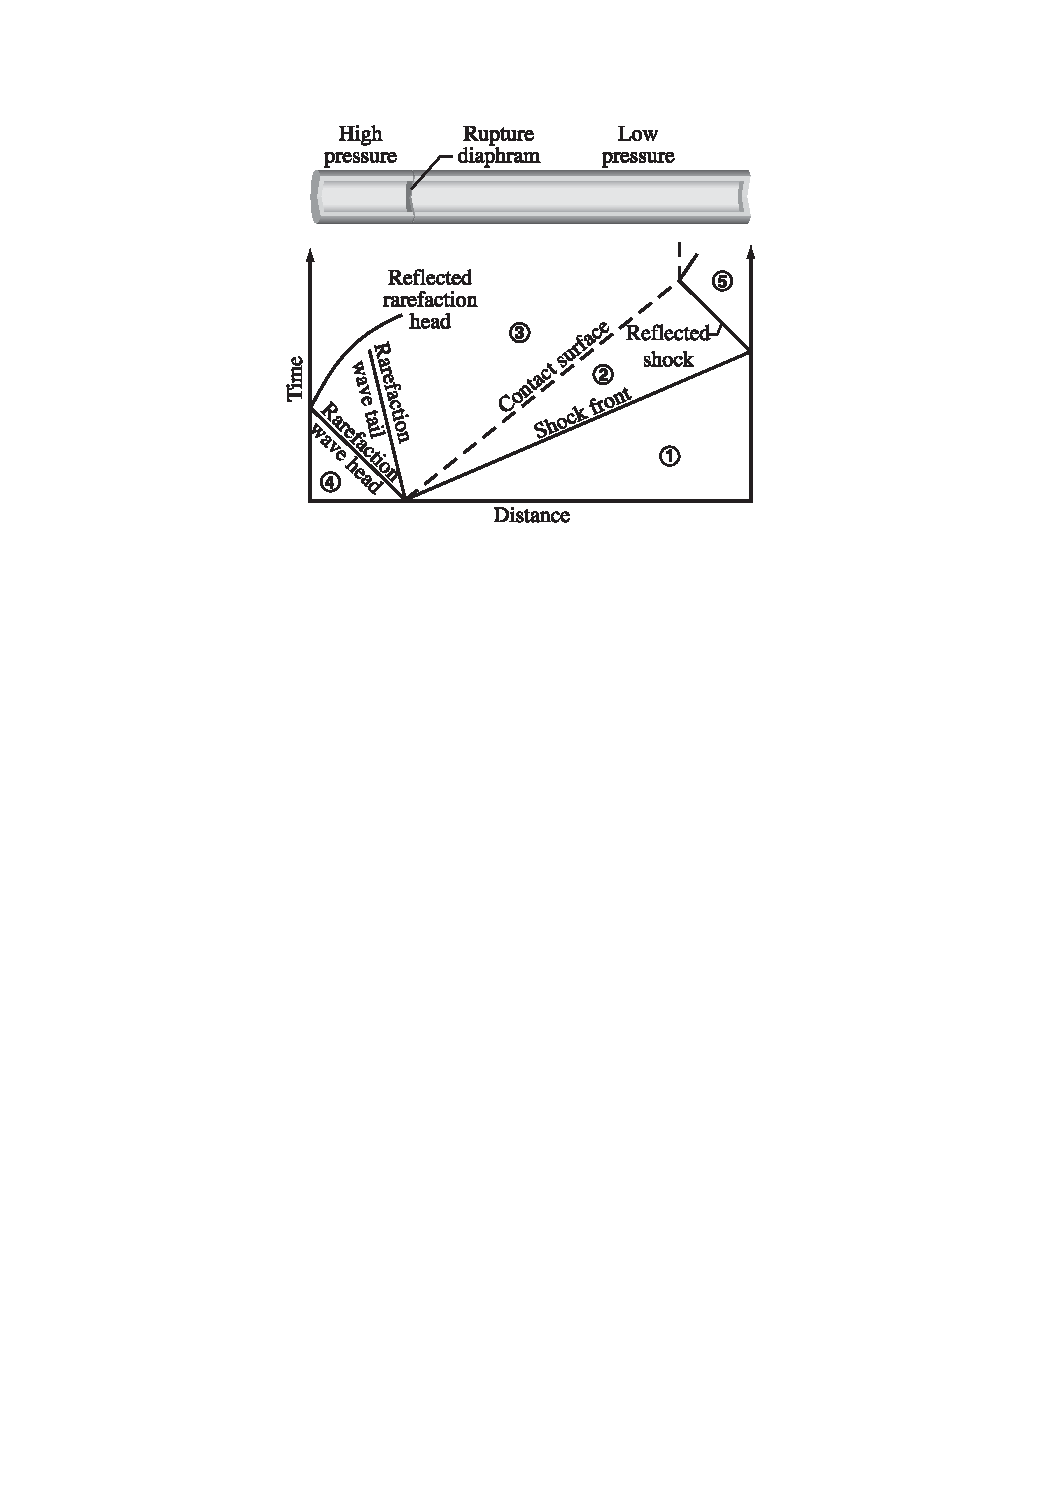
\includegraphics[width=1\textwidth]{Figures/Results/Shocktube/schematics.pdf}
%	\end{subfigure}
%	\begin{subfigure}[t]{0.4\textwidth}
%		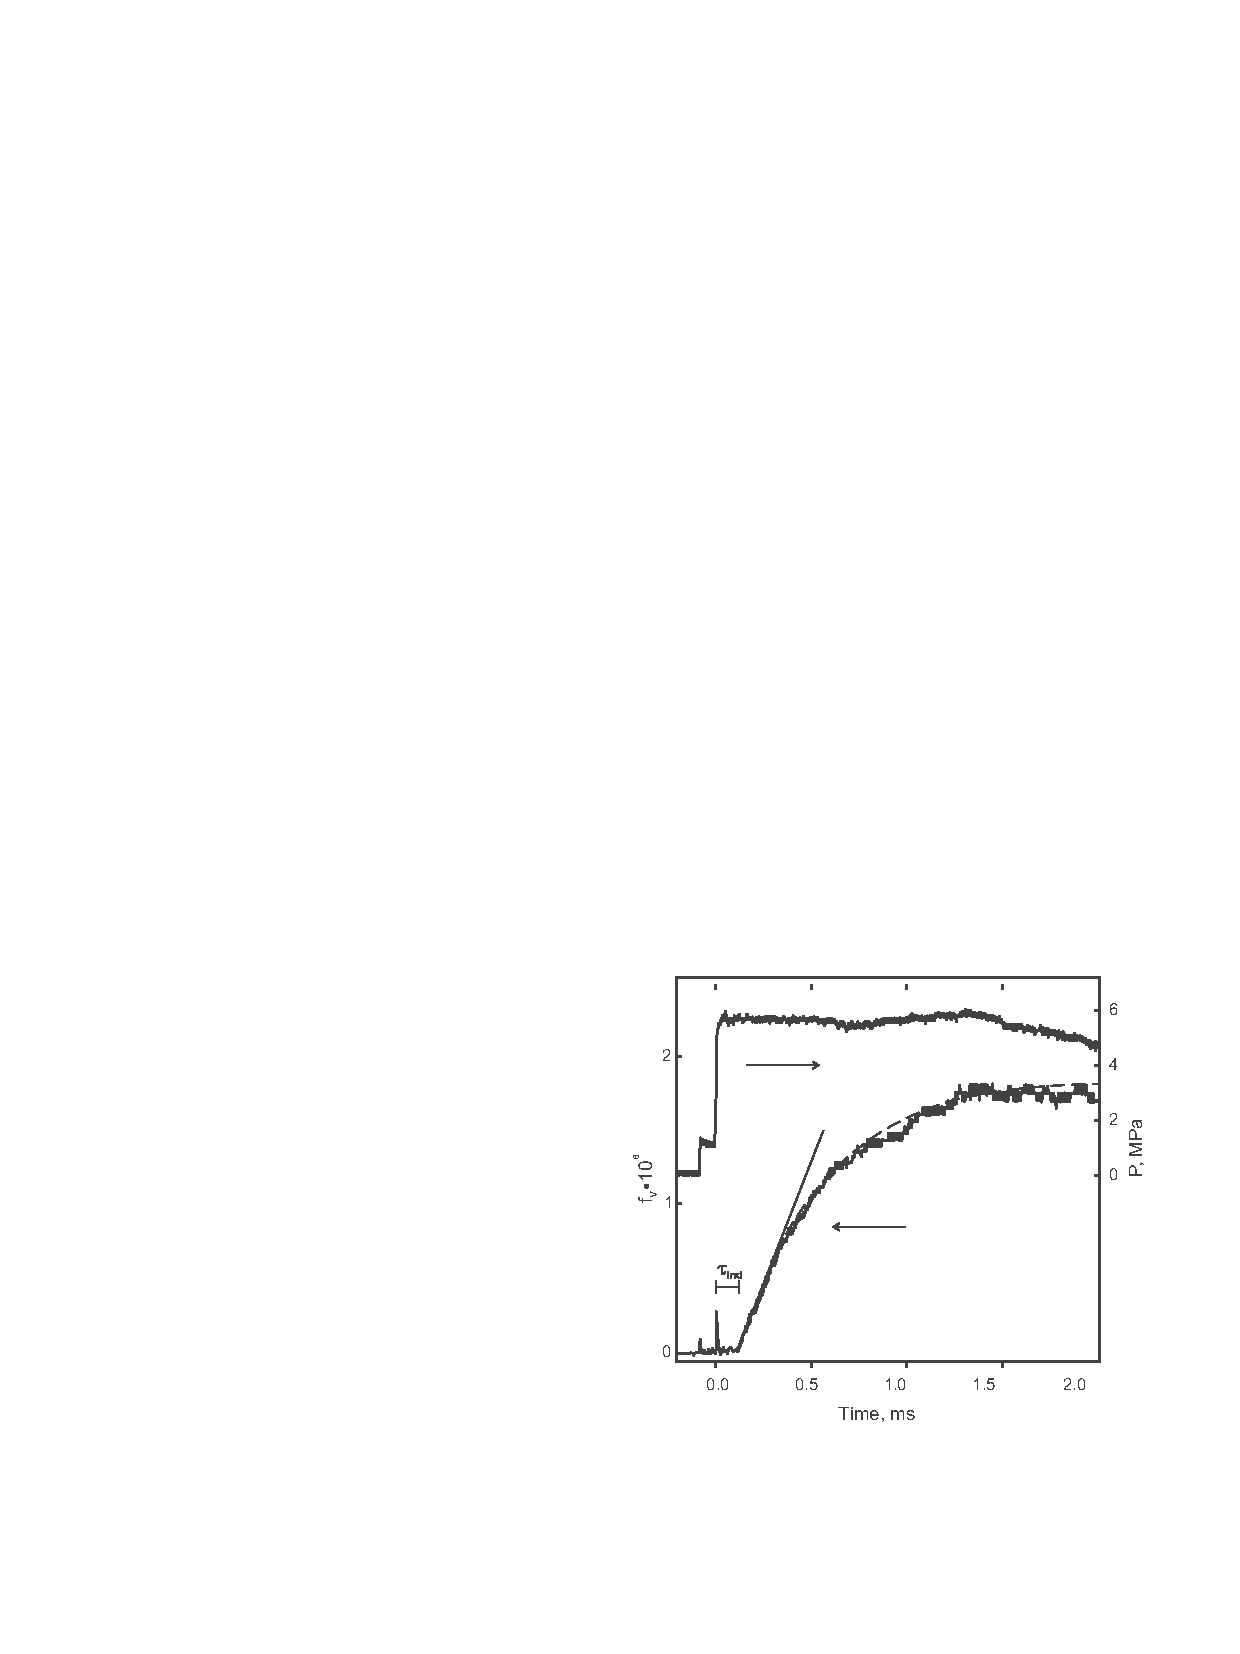
\includegraphics[width=1\textwidth]{Figures/Results/Shocktube/pfv_sample_shocktube.pdf}
%	\end{subfigure}
%	\caption{The schematics of a shock-tube and the idealized shockwave diagram(left pane reprinted from ~\citet{kee2017chemically}) and the variation of soot volume fraction measured by the extinction record at 633 nm and the pressure profile behind the reflected shock wave in a mixture 0.03\% benzene in Ar at T = 1890 K(right pane reprinted from ~\citet{karasevich1994soot})}
%	\label{fig:shocktubeschem}
%\end{figure}

The passage of reflected shock, referred to as region 5 with $\mathrm{T_5}$ and $\mathrm{P_5}$, is the reference for calculation of residence time and the starting point for simulations. The delay in appearance of soot (often quantified by a threshold for LII or extinction signals) is known as induction time, $\mathrm{\tau_{ind}}$. There has been a lot of research in the literature on induction time (similarly on ignition delay time) in shock tubes~\citep{fussey1978shock}, but it is not the focus of this work. Instead, we mainly focus on species concentrations and soot characteristics during the pyrolysis of methane, at atmospheric and higher pressures which can be used for the design and optimization of CB in plasma reactors~\citep{fulcheri2023energy}. 

%----------------------------------------------------------------
%
% STANFORD SHOKCTUBE DATA 30% CH4
%
%----------------------------------------------------------------

\subsection{Experimental setup and data collection}

The experiments on $\mathrm{CH_4}$ pyrolysis were conducted by Hanson Research Group at Stanford University. The data has not been published yet (at the time of writing the document) and were provided through the collaboration with Monolith Materials and Stanford University.

Mole fraction time histories of methane ($\mathrm{CH_4}$), acetylene ($\mathrm{C_2H_2}$), and ethylene ($\mathrm{C_2H_4}$) were captured using continuous wave (CW) laser absorption at 3.365 $\mu$m, 2.998 $\mu$m, and 10.532 $\mu$m, respectively~\citep{pinkowski2019multi, cassady2020thermal, stranic2014laser}. Soot volume fraction was measured using laser light extinction at $\lambda$=633 nm and 1064 nm with absorption function, E(m) of 0.174 and 0.203~\citep{lee1981optical}, respectively. Additionally, soot samples were collected onto imaging stubs mounted in the shock-tube end-wall. A schematic of the experimental setup for laser diagnostics in the shock tube is shown in Fig.~\ref{fig:shocktubelaserlayout}. Samples were extracted from the interior surface of the shock tube endwall after each experiment to allow for imaging and analysis of the particulates. TEM images were recorded with a FEI Tecnai G2 F20 X-TWIN microscope and Gatan SC200 camera for the test case of $\mathrm{P_5}$=4.5 atm and $\mathrm{T_5}$=2217 K.

\begin{figure}[H]
	\centering
	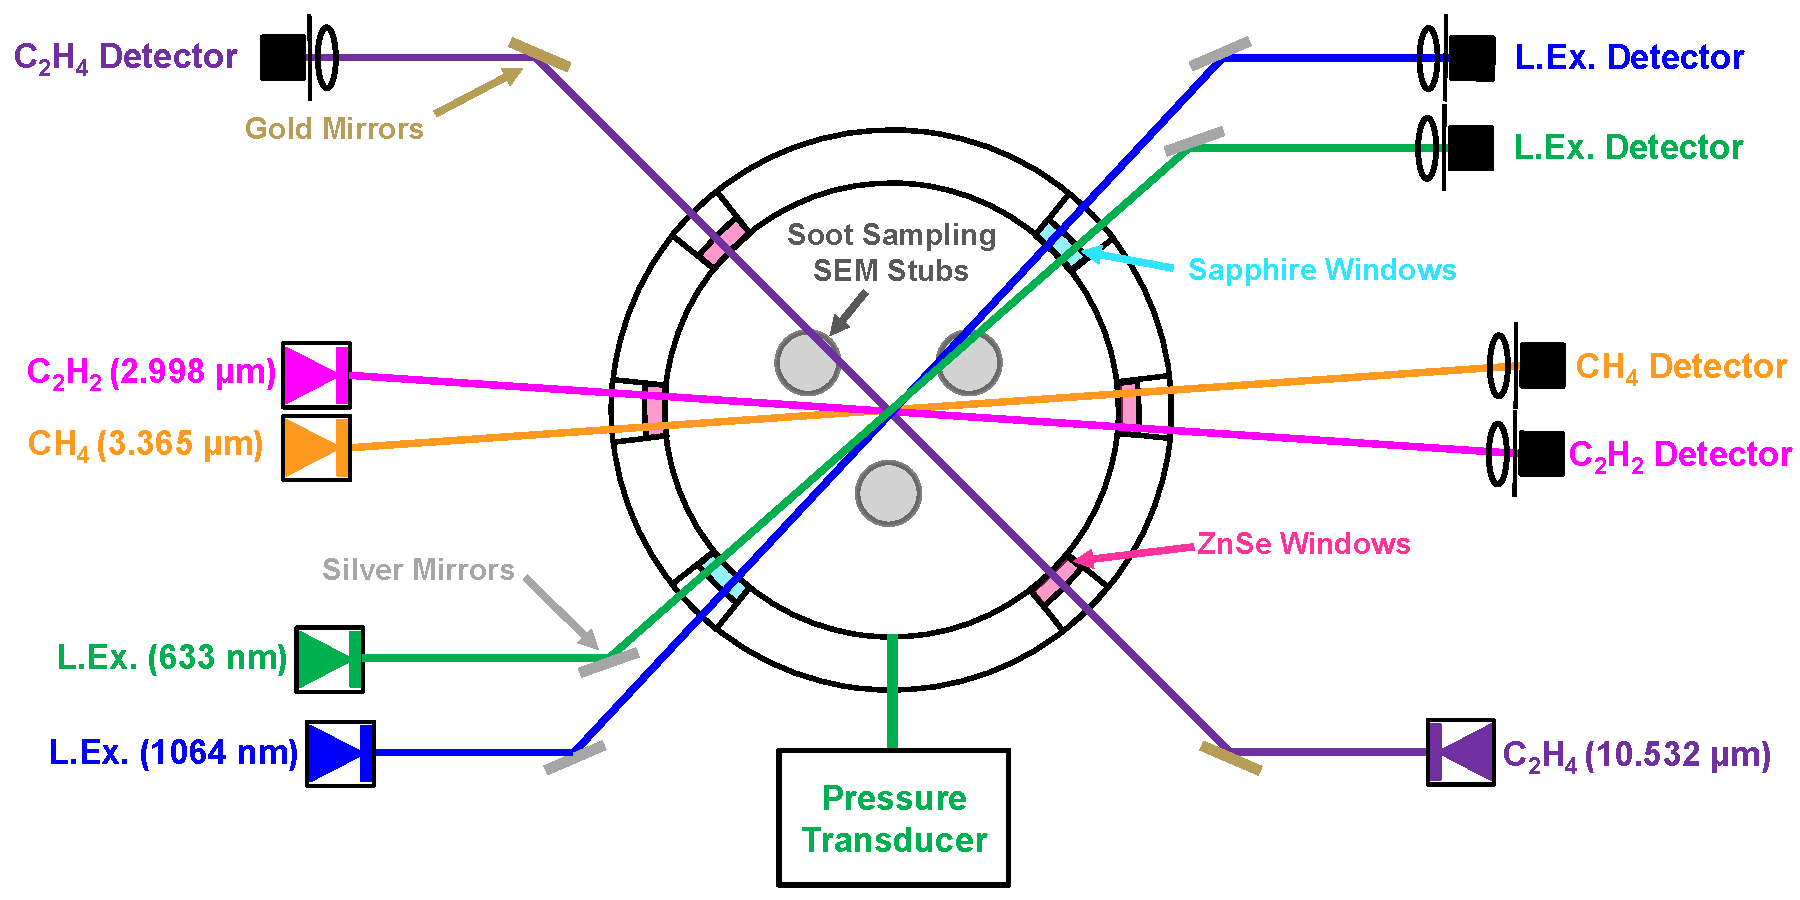
\includegraphics[width=0.75\textwidth]{Figures/Results/Shocktube/laserdiagnostics.pdf}
	\caption{Layout of the laser diagnostics and shock-tube setup. Spatial and spectral filtering is employed to ensure high-quality absorbance measurements to infer species mole fractions and soot volume fraction. Soot samples are collected at the shock-tube endwall. All lasers are aligned in a plane 1 cm from the endwall}
	\label{fig:shocktubelaserlayout} 
\end{figure}

\subsection{30\% Methane Data-set}

The first data set includes eight data points with the fuel loading of 30\% $\mathrm{CH_4}$-Ar at P=4$\pm$0.5 atm in the temperature range of 1800-2500 K. Table~\ref{tab:shocktubest_CH4_30} lists the test conditions including pressure, temperature and composition of all data points.


\begin{table}[H]
	\caption{The pressure, temperature and composition of simulation data points for 30\% $\mathrm{CH_4}$}
	\centering
	\begin{tabular}{l|llllllll|}
		\cline{2-9}
     	& \multicolumn{8}{c|}{Datapoints}                       \\ \cline{2-9} 
		& (1)  & (2)  & (3)  & (4)  & (5)  & (6)  & (7)  & (8)  \\ \hline
		\multicolumn{1}{|l|}{T {[}K{]}}   & 1861 & 1917 & 2030 & 2155 & 2184 & 2313 & 2375 & 2455 \\ \hline
		\multicolumn{1}{|l|}{P {[}atm{]}} & 4.12 & 3.74 & 3.56 & 3.93 & 3.62 & 3.58 & 3.75 & 3.47 \\ \hline
		\multicolumn{1}{|l|}{Composition} & \multicolumn{8}{c|}{$\mathrm{CH_4}$: 0.3, Ar: 0.7}               \\ \hline
	\end{tabular}
	\label{tab:shocktubest_CH4_30} 
\end{table}

 The time history of $\mathrm{CH_4}$, $\mathrm{C_2H_4}$ and $\mathrm{C_2H_2}$ mole fraction as well as soot yield and volume fraction were reported up to 0.5 ms. The constant volume reactor of omnisoot was used with all PAH growth and particle dynamics models. The performance of reaction mechanisms are assessed by comparing the mole fraction of species captured by laser diagnostics, $\mathrm{CH_4}$, $\mathrm{C_2H_4}$, and $\mathrm{C_2H_2}$ with model predictions using Caltech~\citep{blanquart2009chemical}, KAUST~\cite{wang2013pah} and ABF~\citep{appel2000kinetic} mechanisms. The analysis of simulation results (see Figs.~\ref{fig:shocktubest_30ch4_ch4_0}-\ref{fig:shocktubest_30ch4_ch4_0}) showed that soot formation described by different PAH growth and particle dynamcis models have negligible impact on prediction the mole fraction of measured species in the studied temperature range. Therefore, the assessment of reaction mechanisms for prediction of major species is performed without soot to simply the analysis. Figs.~\ref{fig:shocktubest_30ch4_ch4_nosoot_subset}-\ref{fig:shocktubest_30ch4_c2h2_nosoot_subset} compares the mole fraction of $\mathrm{CH_4}$, $\mathrm{C_2H_4}$, $\mathrm{C_2H_2}$ predicted by Caltech, KAUST, and ABF with data from laser diagnostics. Note that only a subset of simulations are shown for brevity, and results for the whole temperature range can be found in Figs.~\ref{fig:shocktubest_30ch4_nosoot_ch4}-\ref{fig:shocktubest_30ch4_nosoot_c2h2}. $\mathrm{CH_4}$ mole fraction starts with a sharp drop from 0.3 at the beginning (corresponding to fast decomposition of methane) followed by a more gradual decrease. The initial decomposition rate increases with temperature. All mechanisms underpredict $\mathrm{CH_4}$ mole fraction, but ABF mechanism predictions are closer to the measurements than KAUST and Caltech. In other words, KAUST and Caltech overestimate $\mathrm{CH_4}$ conversion rate.
 %directing more carbon towards larger hydrocarbons and PAHs. 
 The mole fraction of $\mathrm{C_2H_4}$ (Fig.\ref{fig:shocktubest_30ch4_c2h4_nosoot_subset}) starts with a quick jumps after methane decomposition, reaches the maximum value and gradually decreases towards its final value. The simulations extended beyond test time of shock-tube calculations showed that $\mathrm{C_2H_4}$ mole fraction predicted by KAUST and Caltech mechanisms continues to decrease to the equilibrium values, but ABF predicts an increase at longer residence times indicating reversal of $\mathrm{C_2H_4}$ decomposition which is more pronounced at high temperatures. The $\mathrm{C_2H_2}$ mole fraction increases in two steps, a rapid increase at the beginning followed by a gradual one. ABF mechanism predictions are in good agreement with measurements, but Caltech and KAUST underpredict the $\mathrm{C_2H_2}$ mole fraction. The difference between mechanisms are more pronounced at equilibrium conditions. While ABF predicts a plateau beyond 1.5 ms, KAUST and Caltech predict a decrease towards a lower value indicating conversion of acetylene to larger hydrocarbons and PAHs. The carbon mass fraction (CMF) of measured species, $\mathrm{CH_4}$, $\mathrm{C_2H_4}$ and $\mathrm{C_2H_2}$ combined is shown in Fig.~\ref{fig:shocktubest_30ch4_ccc_nosoot_subset}. The CMF of different mechanisms decreases up to a certain time that shortens with temperature. Beyond that, ABF mechanism predicts an increasing trend indicating that carbon returns to major species, but KAUST and Caltech continuously transfer carbon from measured species to larger hydrocarbons. This is consistent with the CMF of soot precursors shown in Fig.~\ref{fig:shocktubest_30ch4_spc_nosoot_subset}, which is significantly larger for KAUST and Caltech compared with ABF by two to three orders of magnitude, so it is expected that ABF mechanism cannot provide enough precursors for soot model to predict volume fraction comparable with the measurements.  
 \begin{figure}[H]
 	\centering
 	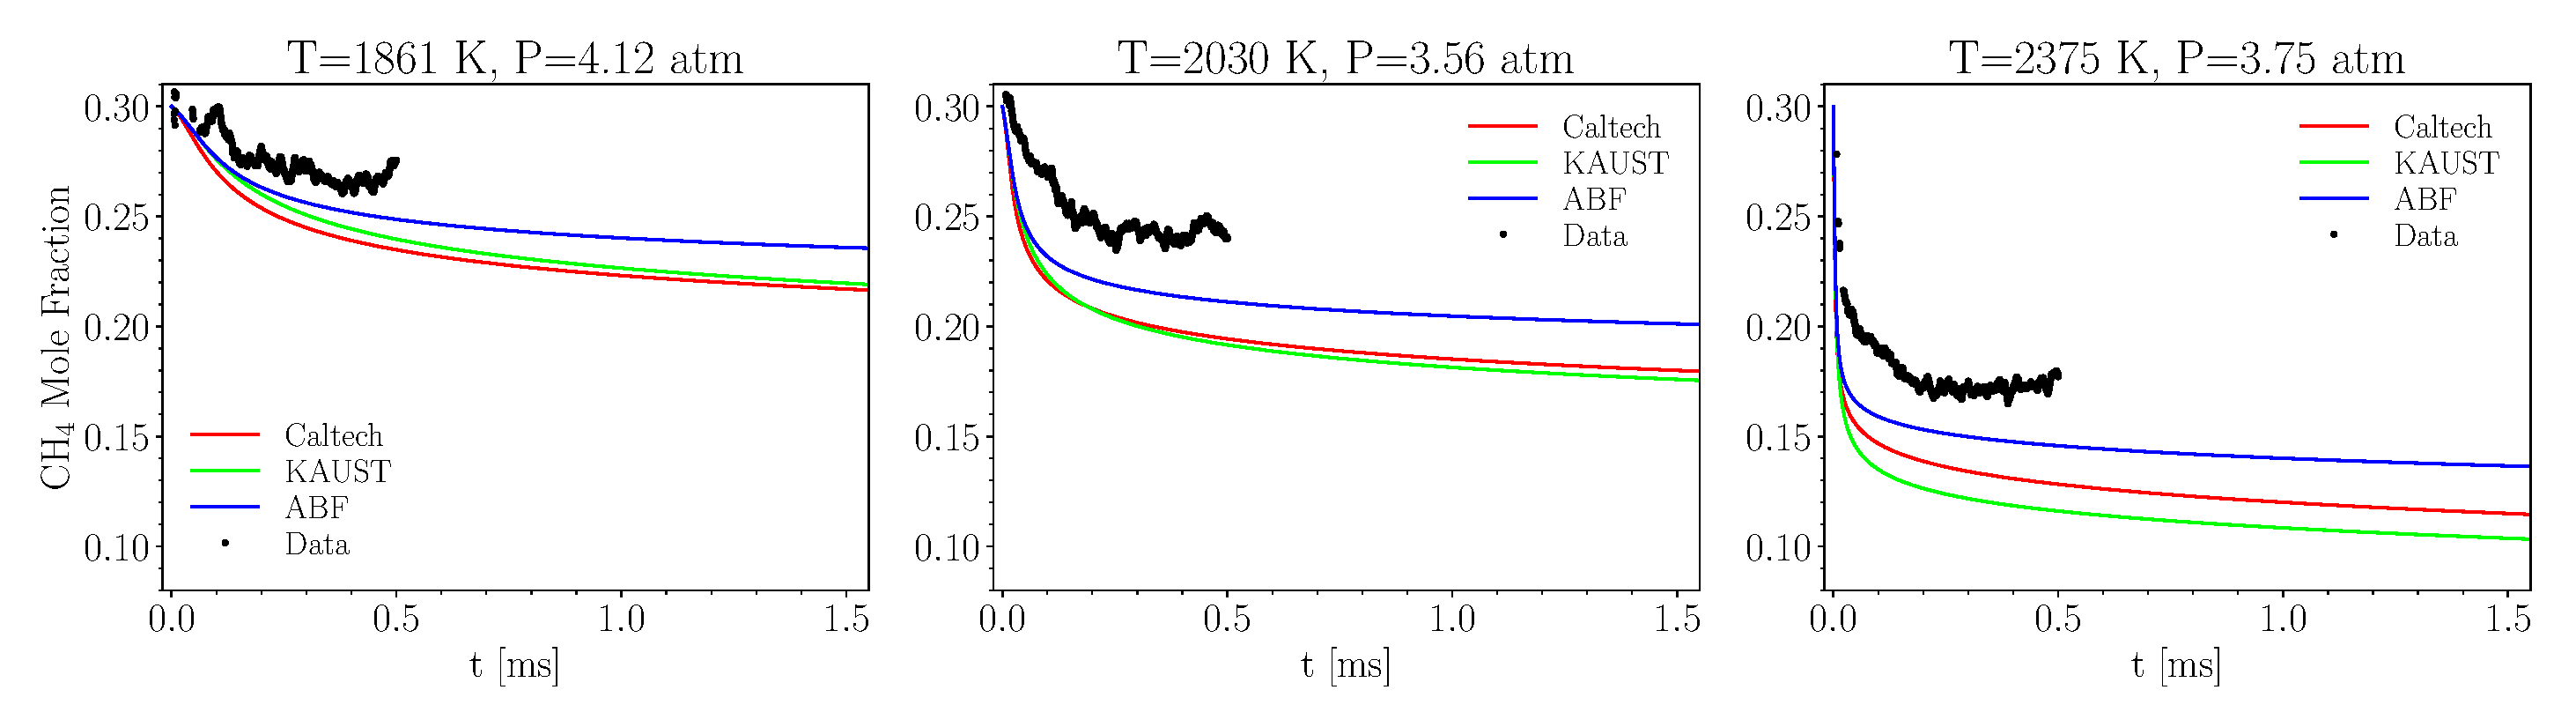
\includegraphics[width=1\textwidth]{Figures/Results/Shocktube/Stanford/june/30CH4_CH4_mechs_nosoot_subset.pdf}
 	\caption{The time history of carbon mass fraction of $\mathrm{CH_4}$ of 30\% $\mathrm{CH_4}$ pyrolysis at T=1861, 2083, and 2375 K using Caltech, KAUST, and ABF mechanisms compared with laser diagnostics data}
 	\label{fig:shocktubest_30ch4_ch4_nosoot_subset} 
 \end{figure}

 \begin{figure}[H]
	\centering
	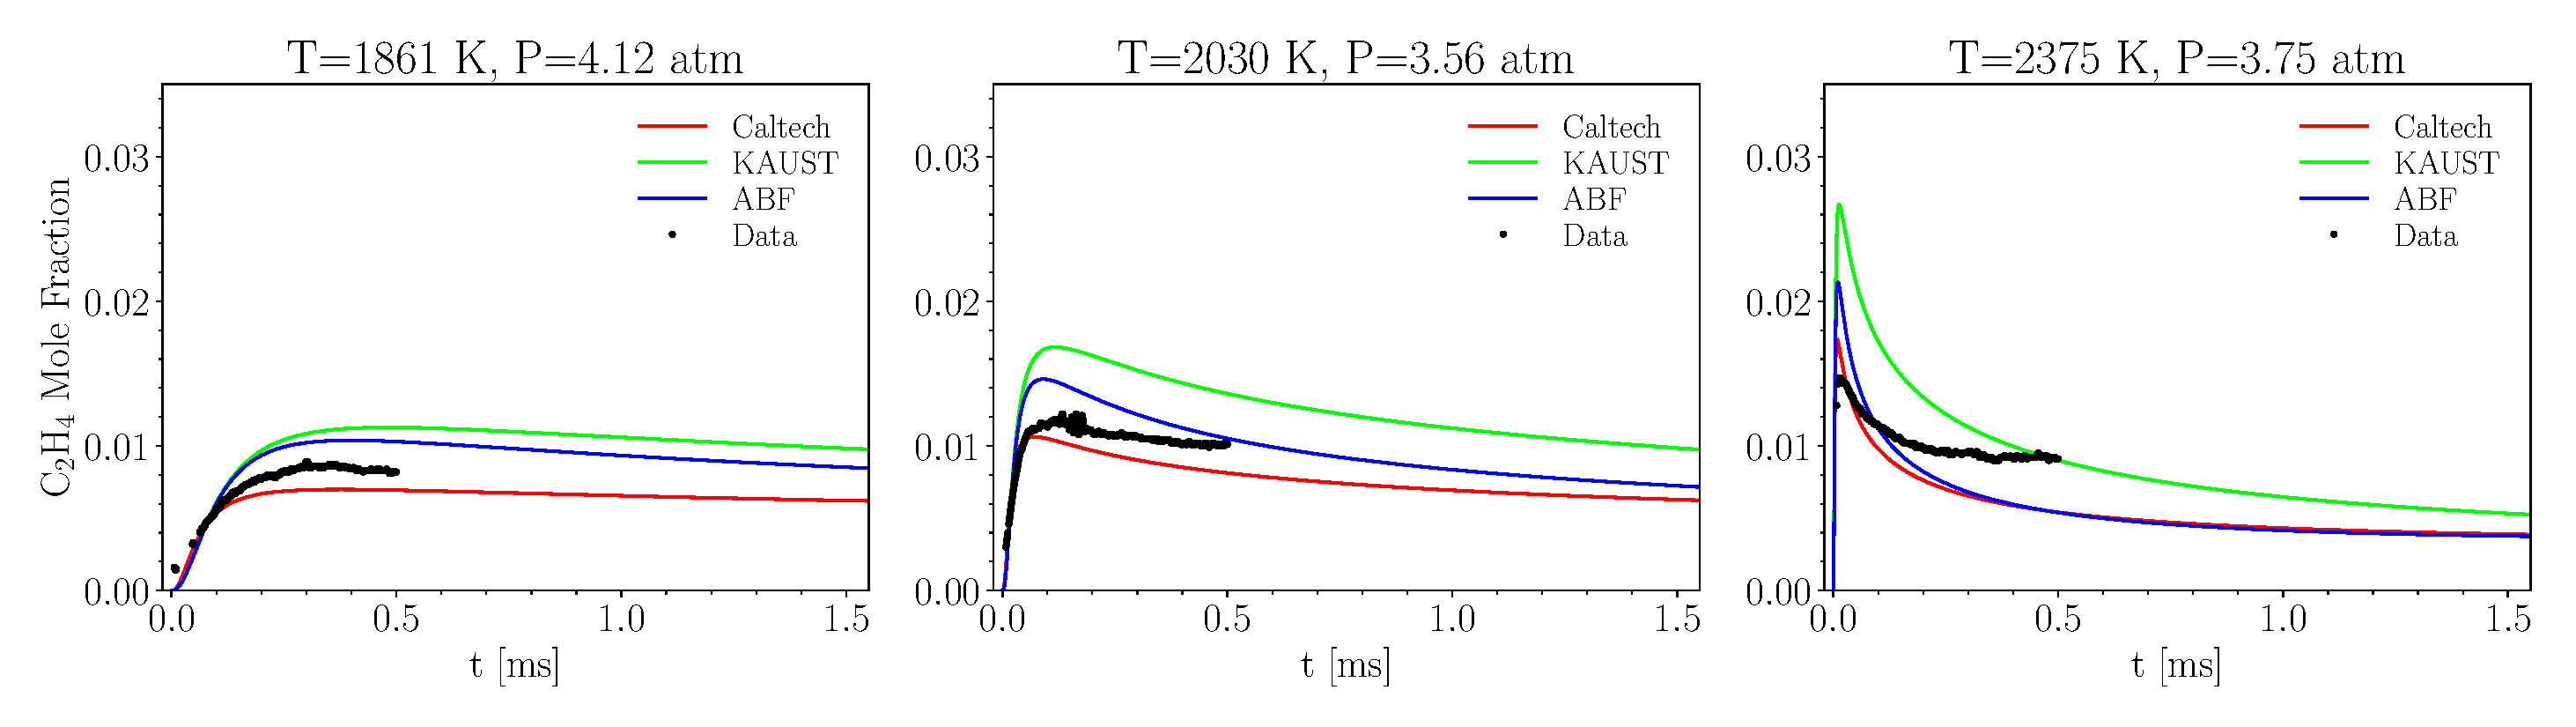
\includegraphics[width=1\textwidth]{Figures/Results/Shocktube/Stanford/june/30CH4_C2H4_mechs_nosoot_subset.pdf}
	\caption{The time history of carbon mass fraction of $\mathrm{C_2H_4}$ of 30\% $\mathrm{CH_4}$ pyrolysis at T=1861, 2083, and 2375 K using Caltech, KAUST, and ABF mechanisms compared with laser diagnostics data}
	\label{fig:shocktubest_30ch4_c2h4_nosoot_subset} 
\end{figure}

 \begin{figure}[H]
	\centering
	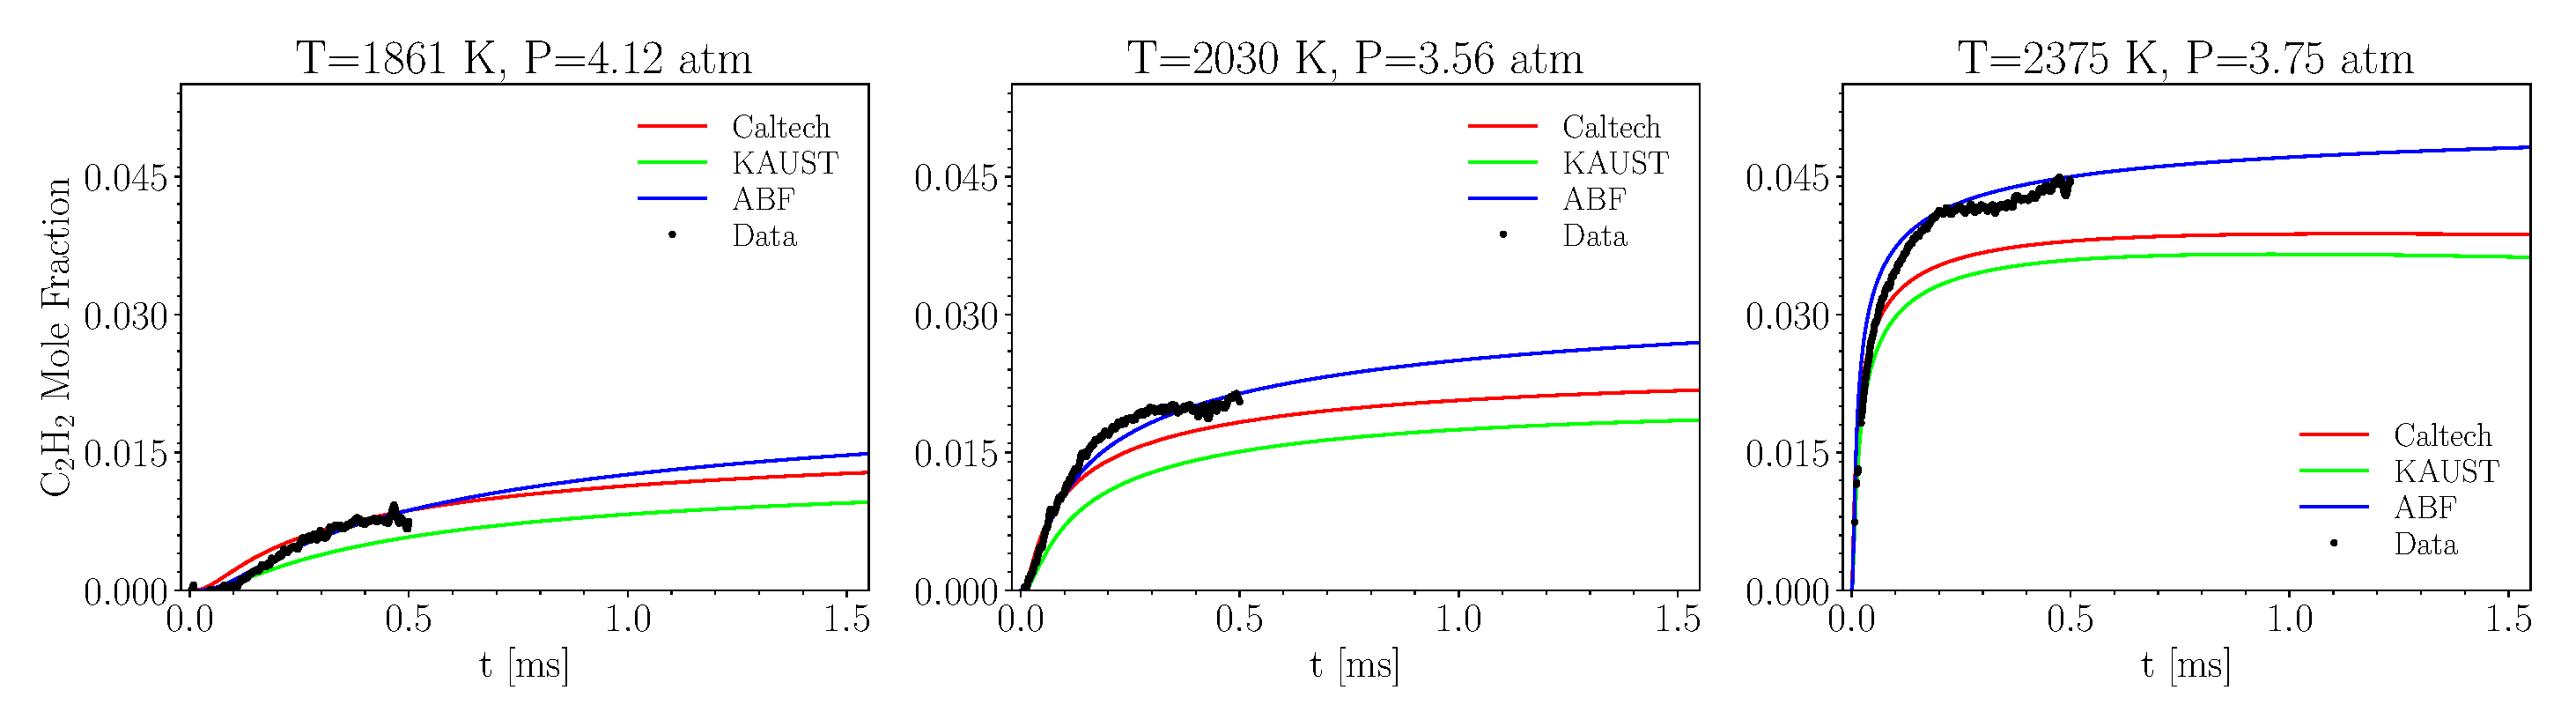
\includegraphics[width=1\textwidth]{Figures/Results/Shocktube/Stanford/june/30CH4_C2H2_mechs_nosoot_subset.pdf}
	\caption{The time history of carbon mass fraction of $\mathrm{C_2H_2}$ of 30\% $\mathrm{CH_4}$ pyrolysis at T=1861, 2083, and 2375 K using Caltech, KAUST, and ABF mechanisms compared with laser diagnostics data}
	\label{fig:shocktubest_30ch4_c2h2_nosoot_subset} 
\end{figure}
 
 
\begin{figure}[H]
	\centering
	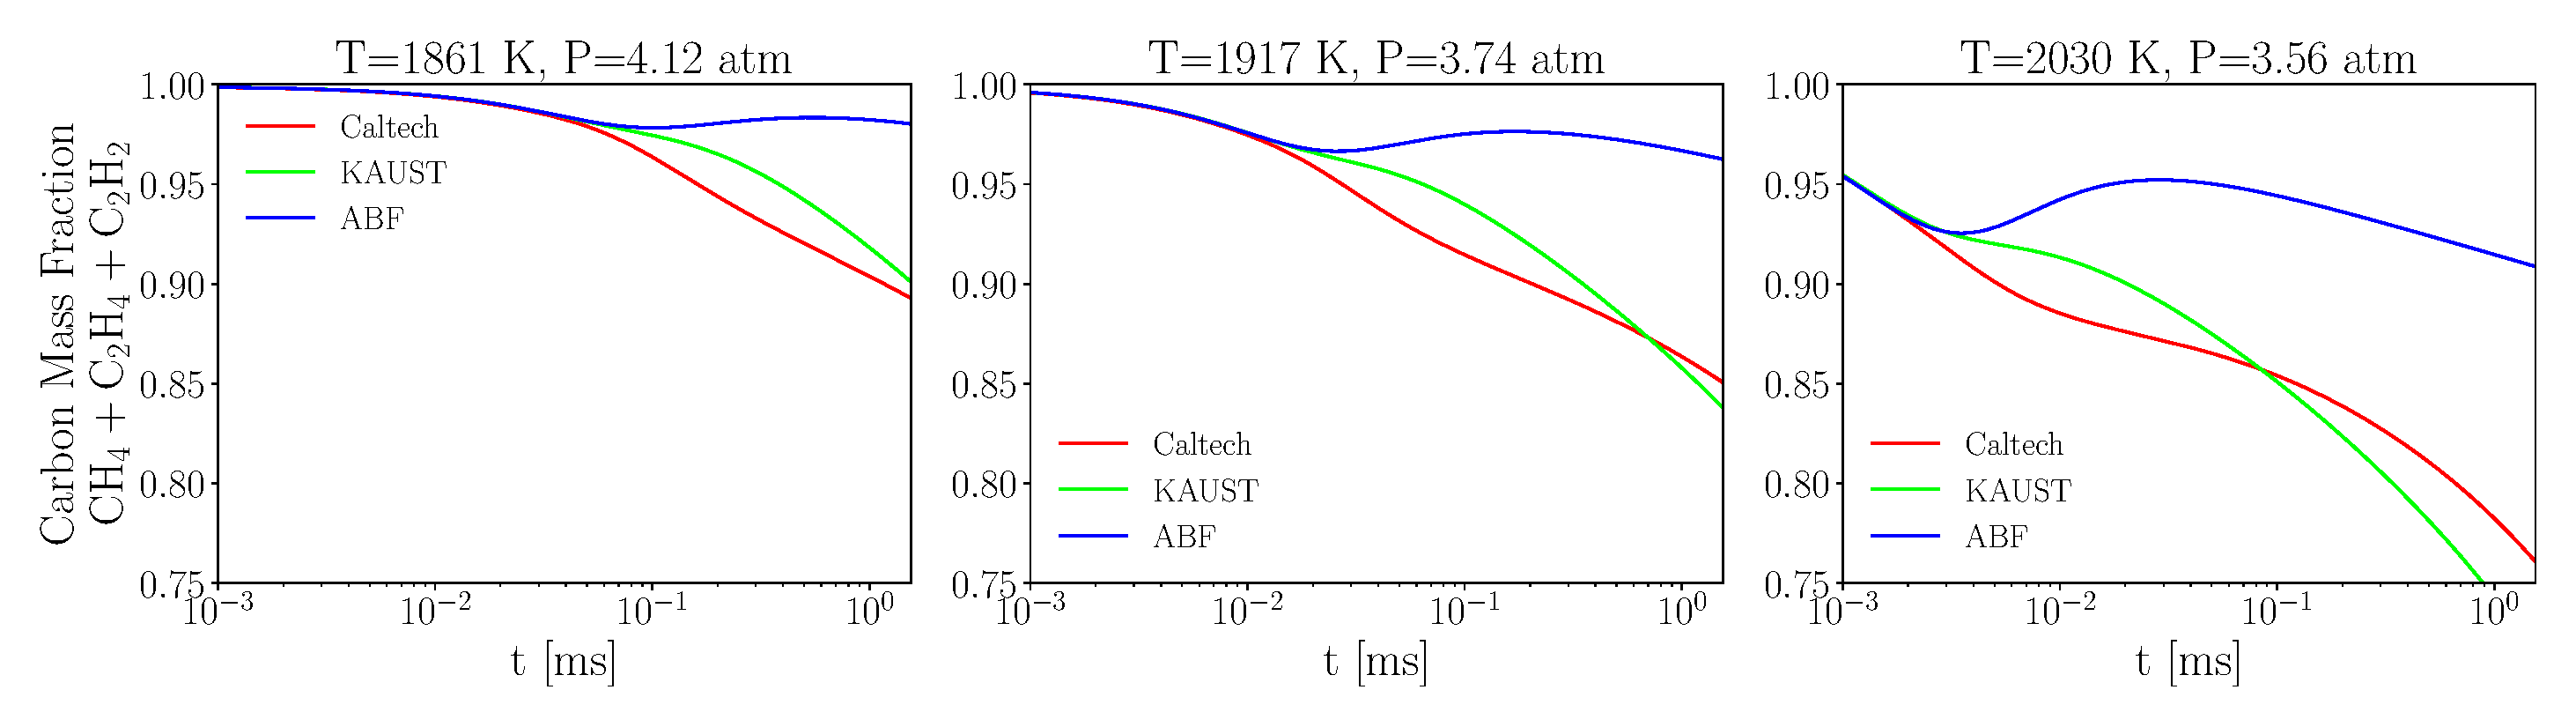
\includegraphics[width=1\textwidth]{Figures/Results/Shocktube/Stanford/june/30CH4_CCC_mechs_nosoot_subset.pdf}
	\caption{The time history of carbon mass fraction of $\mathrm{CH_4}$, $\mathrm{C_2H_4}$, $\mathrm{C_2H_2}$ of 30\% $\mathrm{CH_4}$ pyrolysis at T=1861, 2083, and 2375 K using Caltech, KAUST, and ABF}
	\label{fig:shocktubest_30ch4_ccc_nosoot_subset} 
\end{figure}
 

\begin{figure}[H]
	\centering
	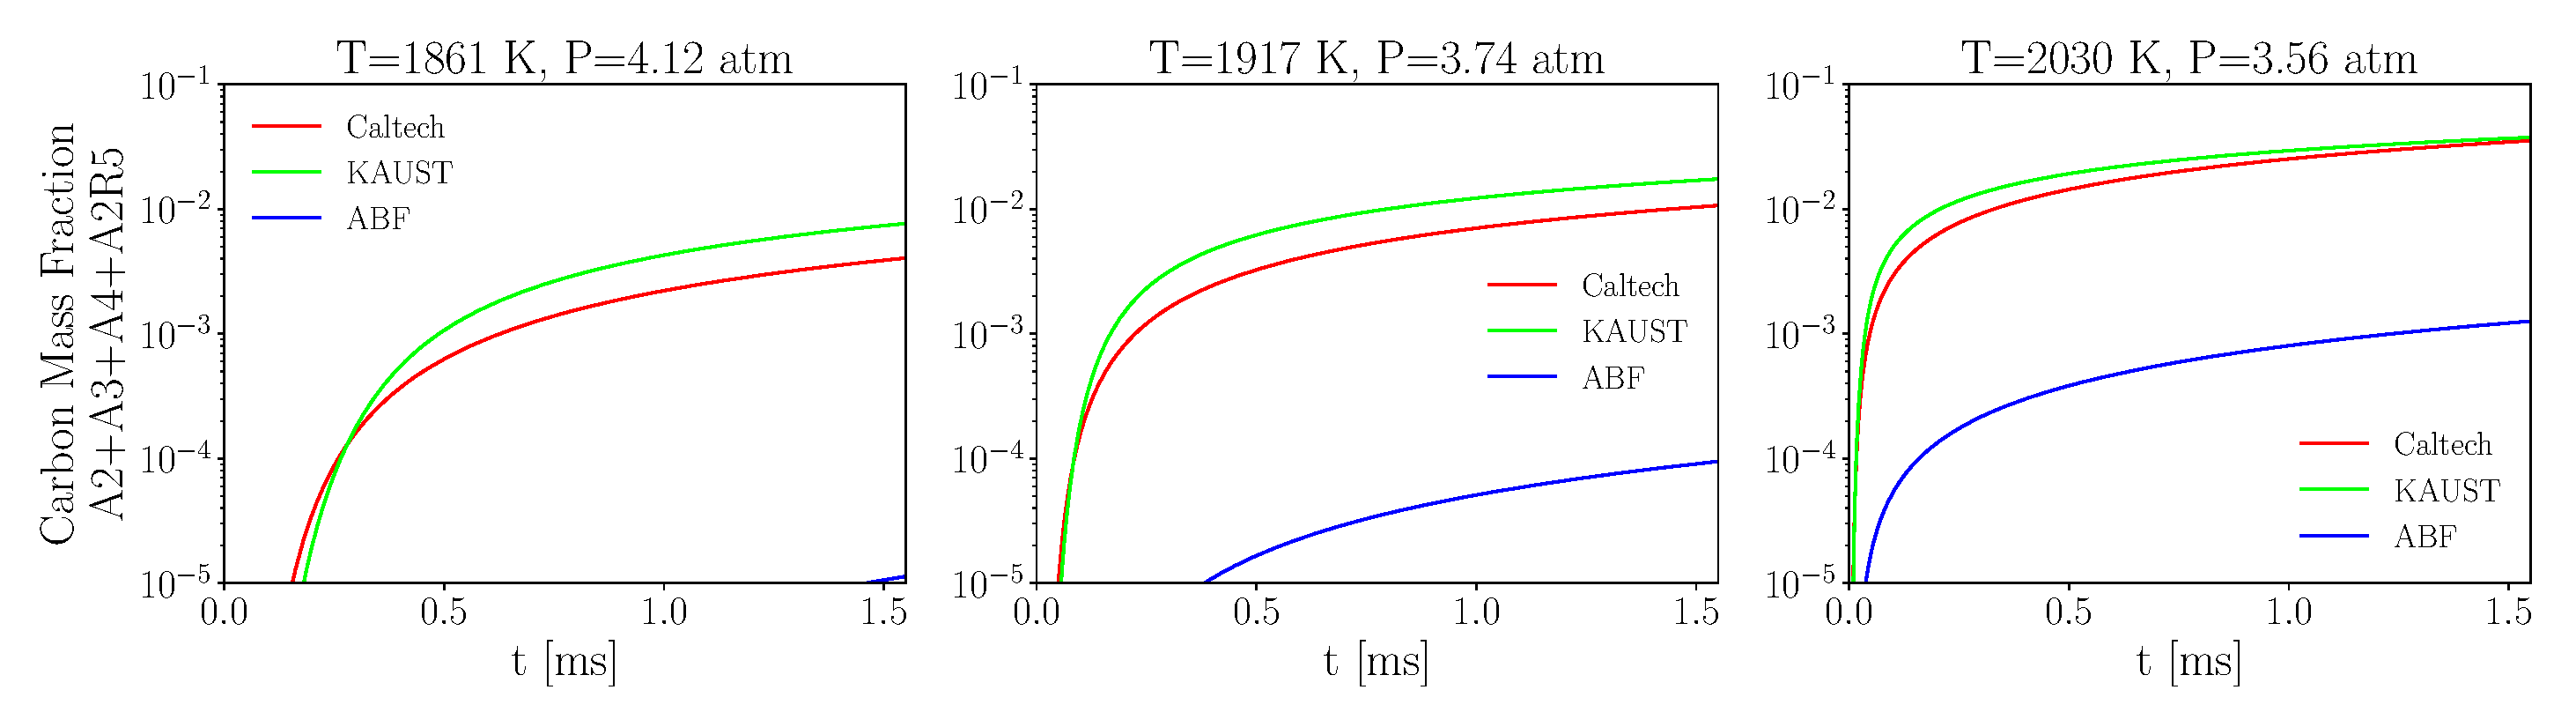
\includegraphics[width=1\textwidth]{Figures/Results/Shocktube/Stanford/june/30CH4_SPC_mechs_nosoot_subset.pdf}
	\caption{The time history of carbon mass fraction of soot precursors, A2, A3, A4 and A2R5 of 30\% $\mathrm{CH_4}$ pyrolysis at T=1861, 2083, and 2375 K using Caltech, KAUST, and ABF mechanisms}
	\label{fig:shocktubest_30ch4_spc_nosoot_subset} 
\end{figure}

Comparing $f_v$ predicted by three reaction mechanisms at T=2375 K and P=3.75 atm with the data from extinction measurements confirms the above-mentioned conclusion. As shown in Fig.~\ref{fig:shocktubest_30ch4_sootvf_single}, the $f_v$ by ABF follows a similar trend as data, but the values are nearly two orders of magnitude lower indicating small PAH concentrations. Although both Caltech and KAUST predict $f_v$ comparable with data, KAUST will be used for detailed soot simulations as its combination with E-Bridge Modified accurately captures soot volume fraction. Having said that, any conclusions drawn using KAUST can be easily generalized to Caltech as well.


\begin{figure}[H]
	\centering
	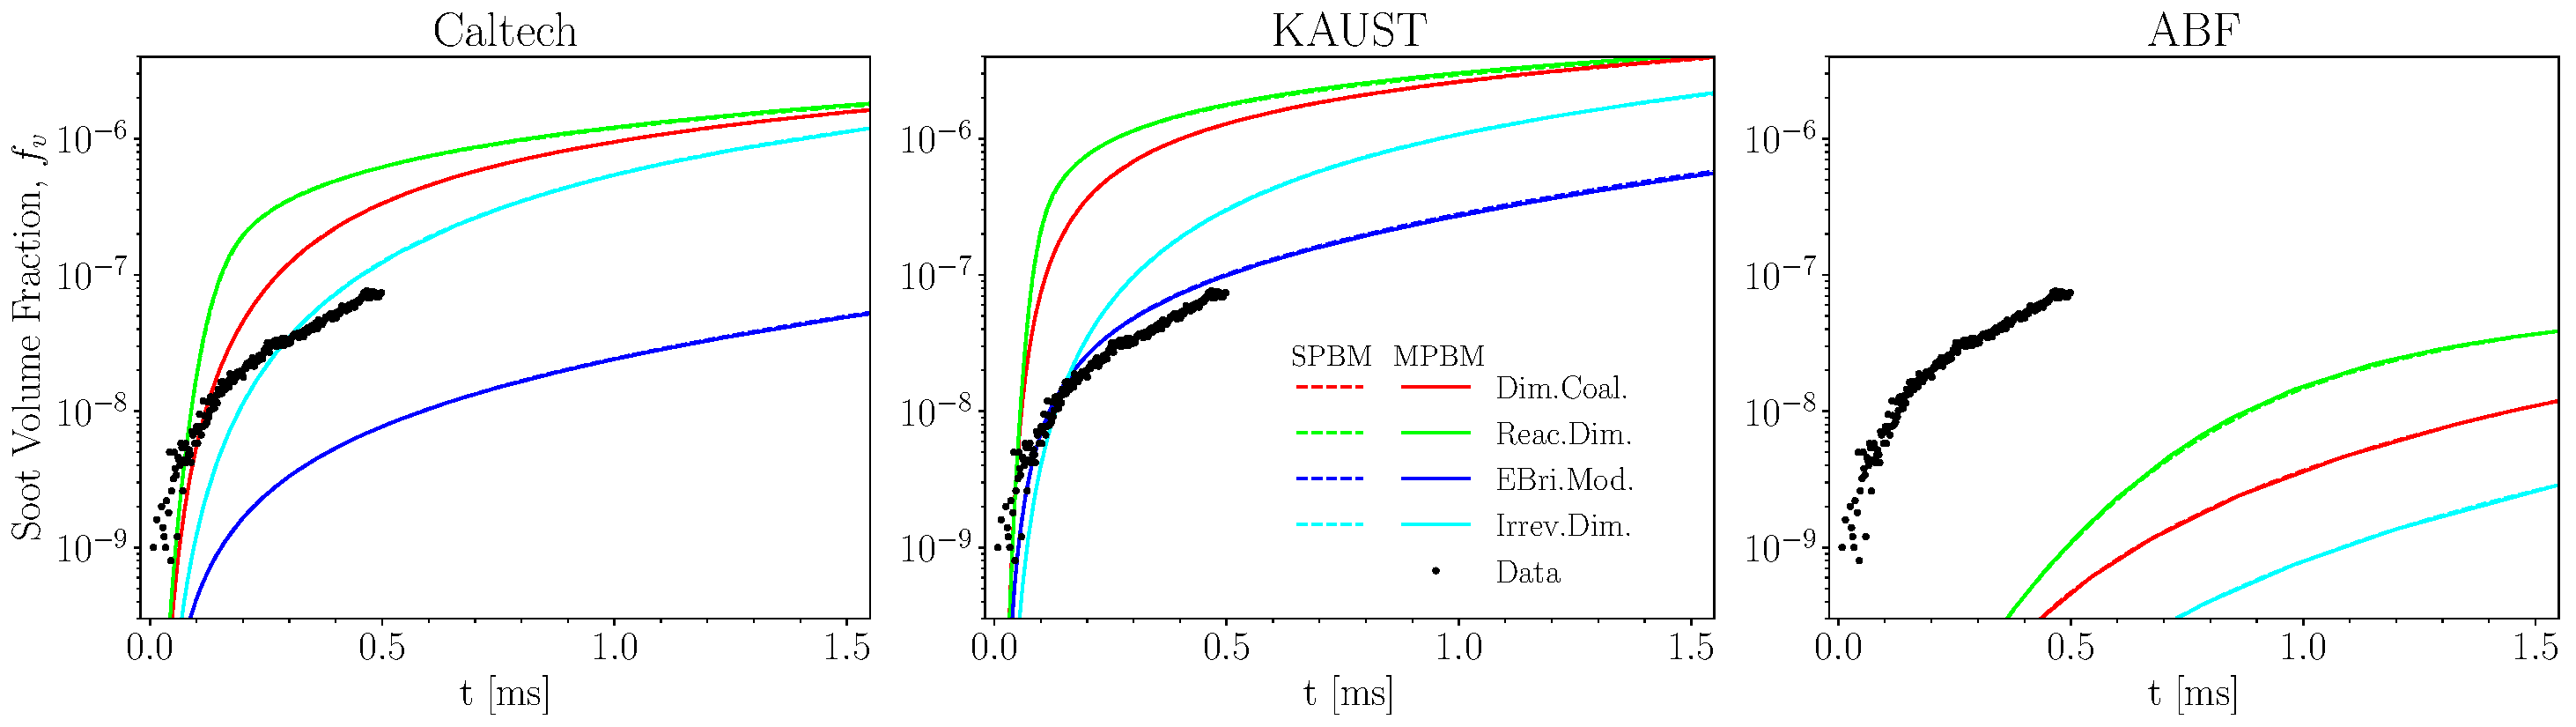
\includegraphics[width=1\textwidth]{Figures/Results/Shocktube/Stanford/june/30CH4_sootvf_mechs_single.pdf}
	\caption{The time history of soot volume fraction of 30\% $\mathrm{CH_4}$ pyrolysis at T=2375 K and P=3.75 atm using Caltech, KAUST, and ABF mechanism and different PAH growth and particle dynamics models}
	\label{fig:shocktubest_30ch4_sootvf_single} 
\end{figure}

Fig.~\ref{fig:shocktubest_30ch4_fv_kaust_subset} shows that the time variation of soot volume fraction in T=2155, 2313, and 2455 K. The measurement data was not available (or too noisy) below 2155 K due to lack of enough soot particles leading to weak extinction signals (see Fig.~\ref{fig:shocktubest_30ch4_fv_kaust}). SPBM and MPBM results coincide indicating that taking polydispersity into account by the particle dynamics model does not affect soot mass during 1.5~ms of simulation. $f_v$ by EBridge Modified is in good agreement with data and the lowest among inception models across the temperature range. On the other hand, Reactive Dimerization and Dimer Coalescence yields the largest $f_v$ nearly two orders of magnitude larger than data (and EBridge Modified). There is a remarkable similarity between trend of $f_v$ and CMF of soot precursors (Fig.~\ref{fig:shocktubest_30ch4_spc_nosoot_subset}) that highlights the major role of inception and PAH adsorption in soot mass growth. Temperature promotes soot formation in the studied shock tube. Fig.~\ref{fig:shocktubest_30ch4_fv_kaust_last} depicts that $f_v$ computed at 1.5 ms increases with temperature in a nearly linear fashion expect for EBridge Modified.

Fig.\ref{fig:shocktubest_30ch4_dp_kaust_subset} shows the time history of primary particle diameter, $d_p$ at different temperatures. For Sectional model, $d_p$ is the average primary particle diameter calculated from arithmetic mean of $d_p$ of all sections. As expected, EBridge Formation and Irreversible Dimerization predict the lowest $d_p$ due to low soot mass growth rate leading to small $f_v$ values. Dimer Coalescence and Reactive Dimerization generate a relatively close $f_v$ values (corresponding to similar soot mass growth), but Reactive Dimerization predicts a larger $d_p$ indicating lower inception flux and stronger PAH adsorption rate of this model compared to Dimer Coalescence. There is a noticeable difference between sectional and monodisperse models in the $d_p$ predicted by Reactive Dimerization, but other inception models do not exhibit such a sensitivity to particle dynamics model. Both models predict the initial rapid rise in $d_p$. While MPBM predicts a gradual increase to final value, $d_p$ by SPBM decreases after the initial rise due to stronger inception rate by SPBM that generates particle with $d_p$=2 nm bringing down the average $d_p$. Fig.~\ref{fig:shocktubest_30ch4_dp_kaust_last} depicts temperature dependence of $d_p$ at 1.5 ms where SPBM predicts a decreasing trend as opposed to MPBM.

% Final fv in terms of temperature
% the time that it taks for each PAH growth model to each 50%/90% of the final value

\begin{figure}[H]
	\centering
	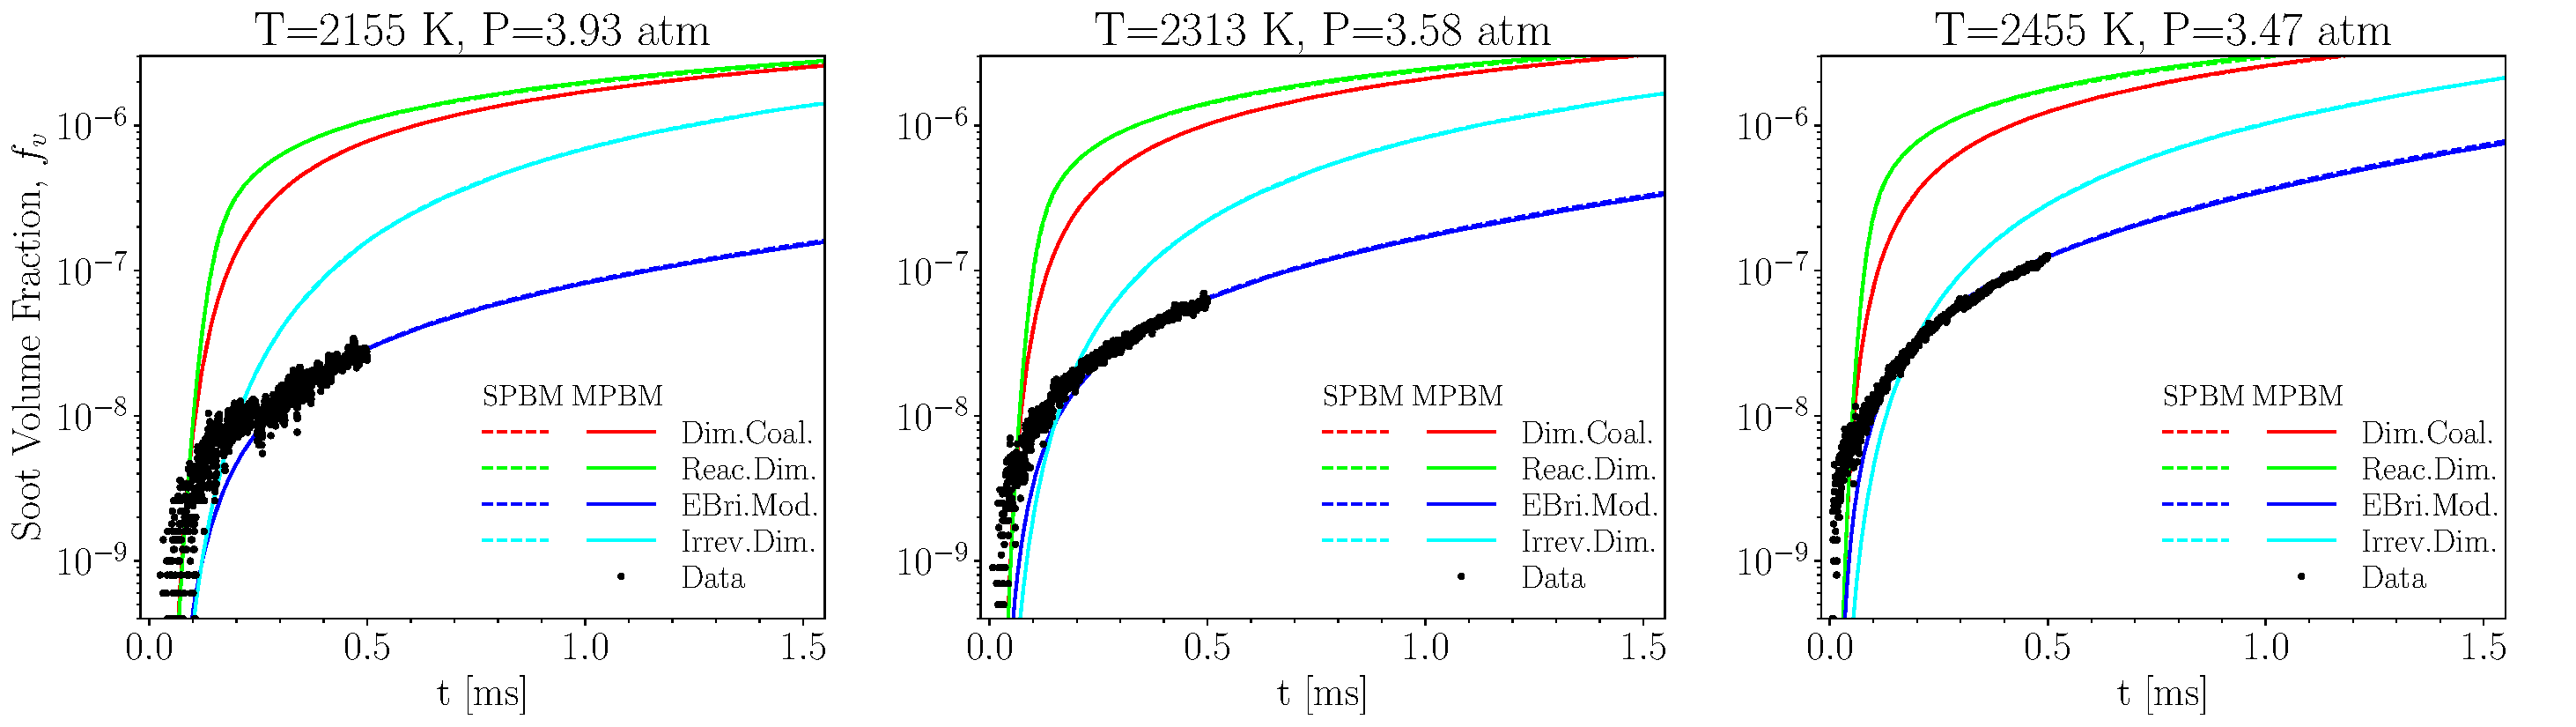
\includegraphics[width=1\textwidth]{Figures/Results/Shocktube/Stanford/june/30CH4_sootvf_kaust_subset.pdf}
	\caption{The time history soot volume fraction, $f_v$ of 30\% $\mathrm{CH_4}$ pyrolysis for T=2155, 2313, and 2455 K using KAUST with different combinations of PAH growth and particle dynamics models compared with extinction measurements}
	\label{fig:shocktubest_30ch4_fv_kaust_subset} 
\end{figure}


\begin{figure}[H]
	\centering
	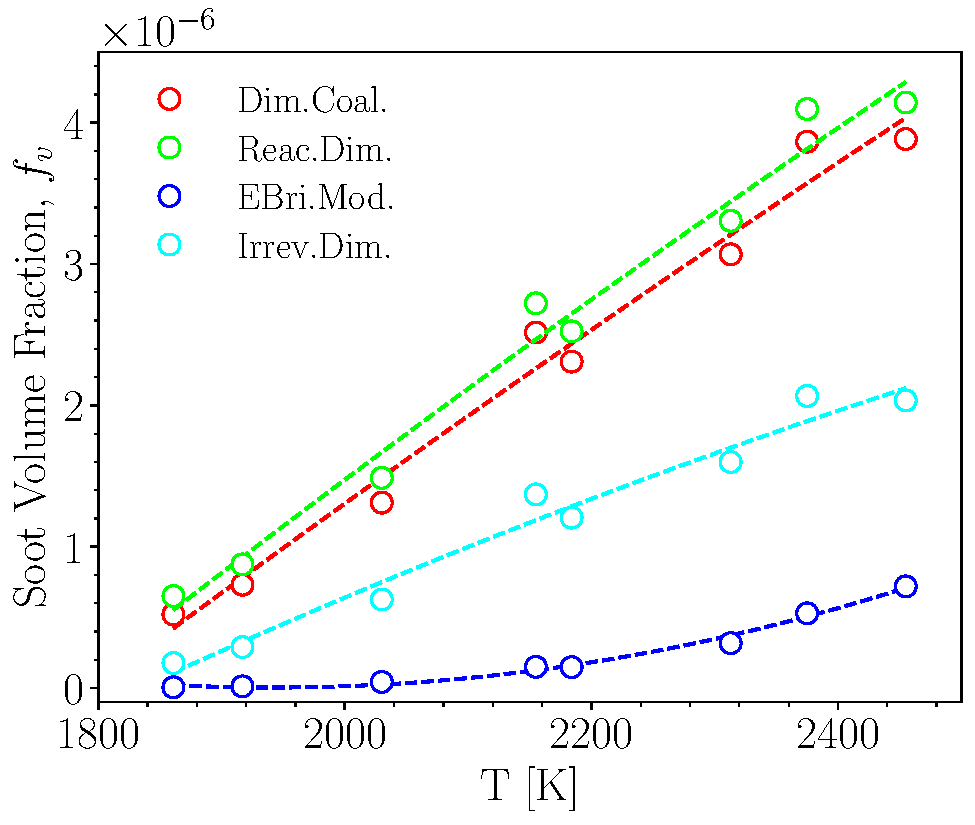
\includegraphics[width=0.32\textwidth]{Figures/Results/Shocktube/Stanford/june/30CH4_sootvf_kaust_1.5ms.pdf}
	\caption{The soot volume fraction, $f_v$ at 1.5 ms increasing with temperature during 30\% $\mathrm{CH_4}$ pyrolysis using KAUST and SPBM. The dashed lines are added to guide the eye}
	\label{fig:shocktubest_30ch4_fv_kaust_last} 
\end{figure}

\begin{figure}[H]
	\centering
	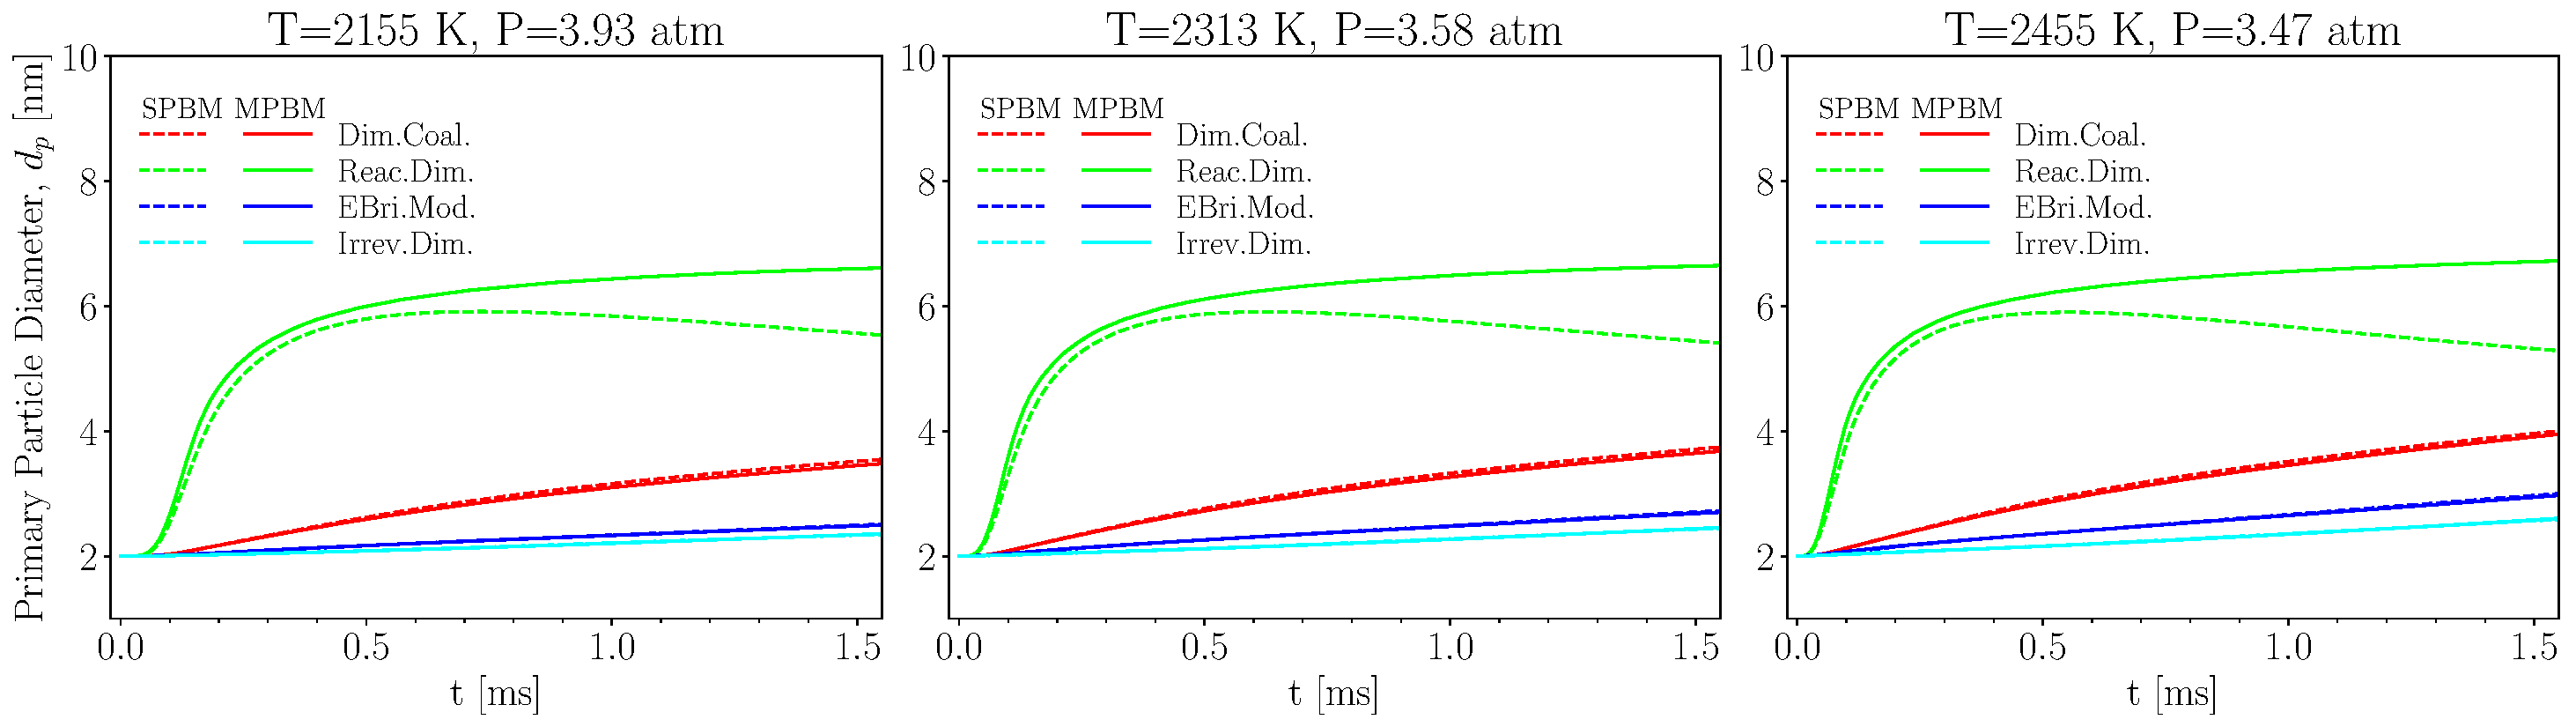
\includegraphics[width=1\textwidth]{Figures/Results/Shocktube/Stanford/june/30CH4_sootdp_kaust_subset.pdf}
	\caption{The time history of primary particle diameter, $d_p$ of 30\% $\mathrm{CH_4}$ pyrolysis for T=2155, 2313, and 2455 K using KAUST with different combinations of PAH growth and particle dynamics models}
	\label{fig:shocktubest_30ch4_dp_kaust_subset} 
\end{figure}

\begin{figure}[H]
	\centering
	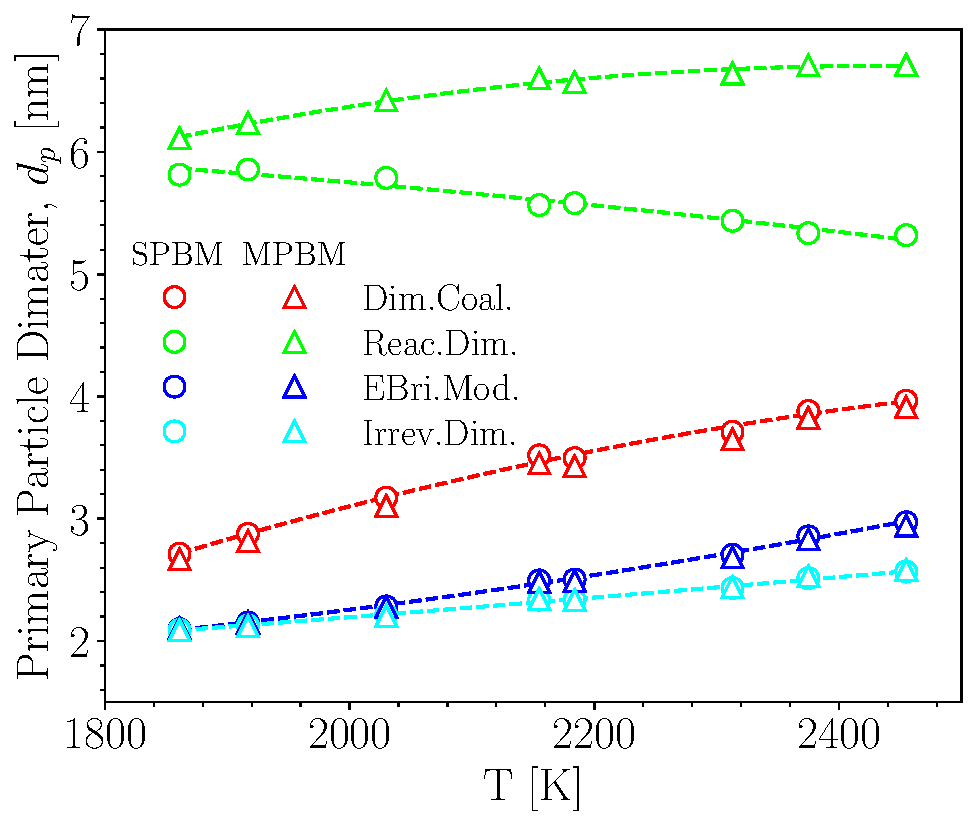
\includegraphics[width=0.32\textwidth]{Figures/Results/Shocktube/Stanford/june/30CH4_sootdp_kaust_1.5ms.pdf}
	\caption{The primary particle diameter, $d_p$ at 1.5 ms increasing with temperature during 30\% $\mathrm{CH_4}$ pyrolysis using KAUST with MPBM and SPBM. The dashed lines are added to guide the eye}
	\label{fig:shocktubest_30ch4_dp_kaust_last} 
\end{figure}

As shown in Fig.~\ref{fig:shocktubest_30ch4_Iinc_kaust_subset}, the inception flux of Reactive Dimerization starts with a quick rise followed by a quick drop until t$\approx$0.25 ms which is nearly the same for both particle dynamics models, but beyond that SPBM predicts an increasing inception flux. This stems from a lower PAH adsorption rate by SPBM (with Reactive Dimerization) directing more PAHs to inception. All models predict an initial rapid rise due to PAH production by $\mathrm{CH_4}$ decomposition. Dimer Coalescence reaches the highest peak and continuously decreases afterward because of consumption of PAHs. However, Irreversible Dimerization and EBridge Modified nearly stay constant towards the end of simulation time. 

\begin{figure}[H]
	\centering
	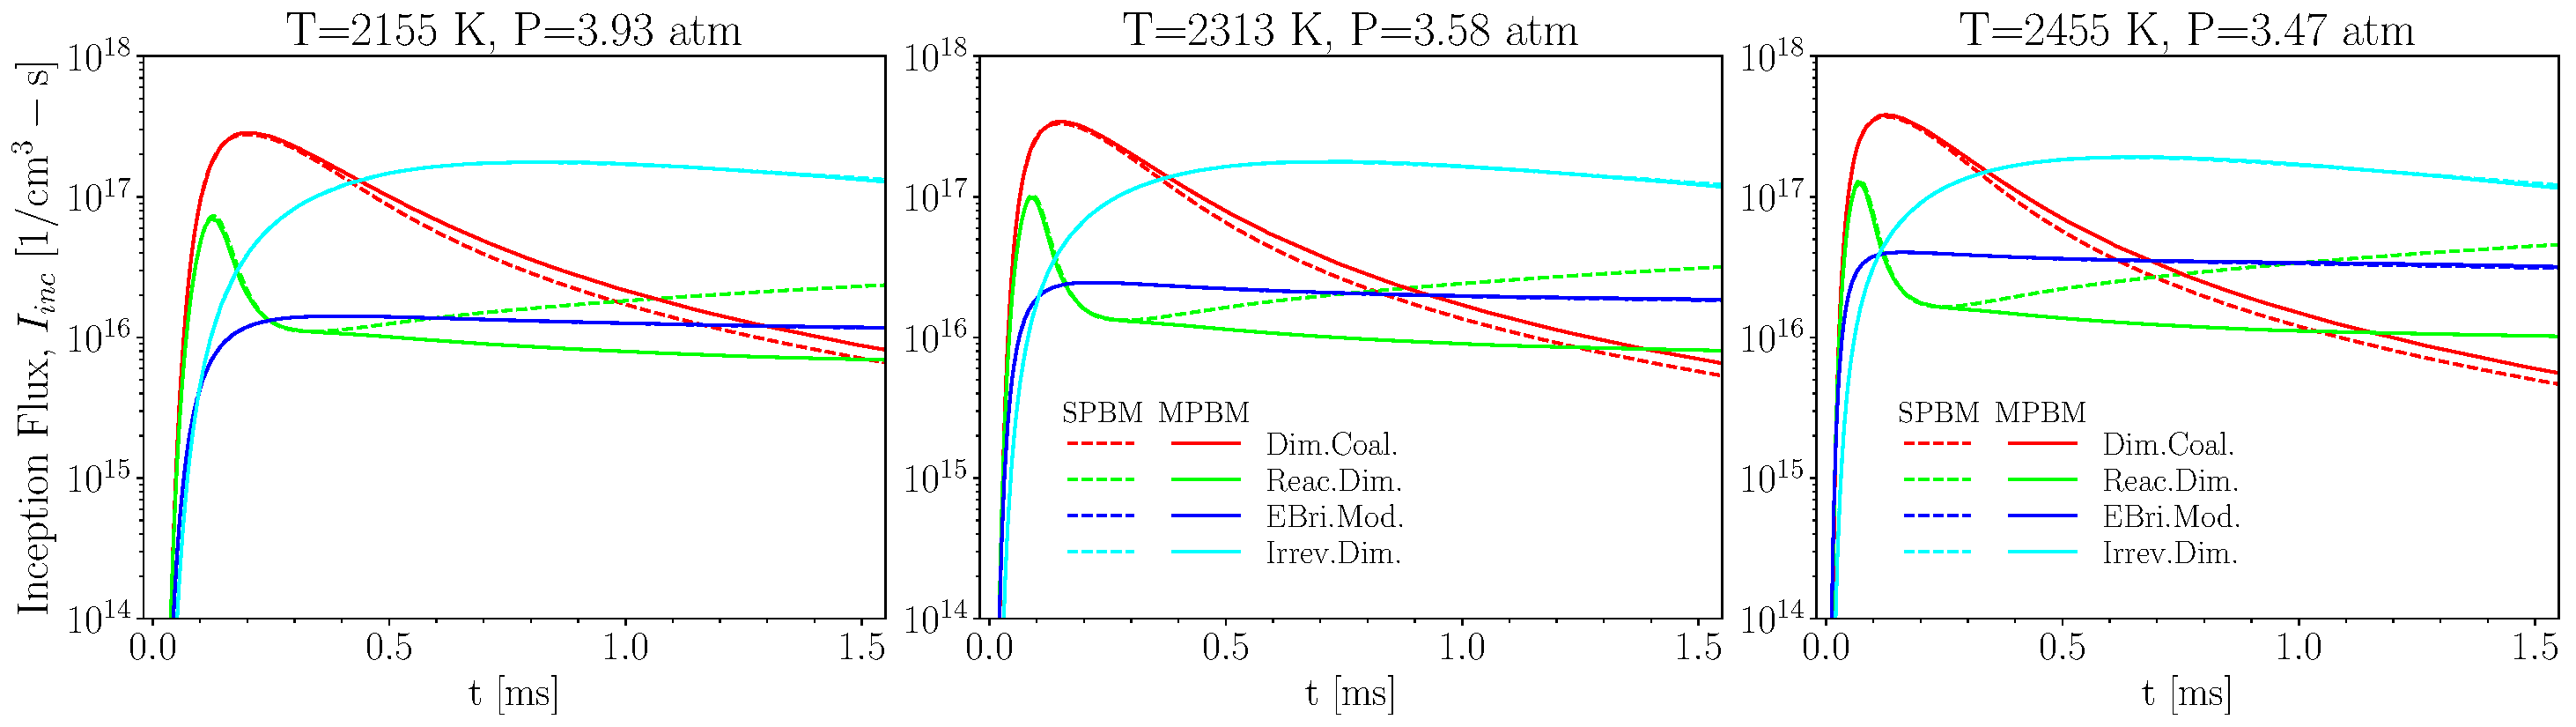
\includegraphics[width=1\textwidth]{Figures/Results/Shocktube/Stanford/june/30CH4_sootIinc_kaust_subset.pdf}
	\caption{The time history of inception flux, $I_{inc}$ of 30\% $\mathrm{CH_4}$ pyrolysis for T=2155, 2313, and 2455 K using KAUST with different combinations of PAH growth and particle dynamics models}
	\label{fig:shocktubest_30ch4_Iinc_kaust_subset} 
\end{figure}

\begin{figure}[H]
	\centering
	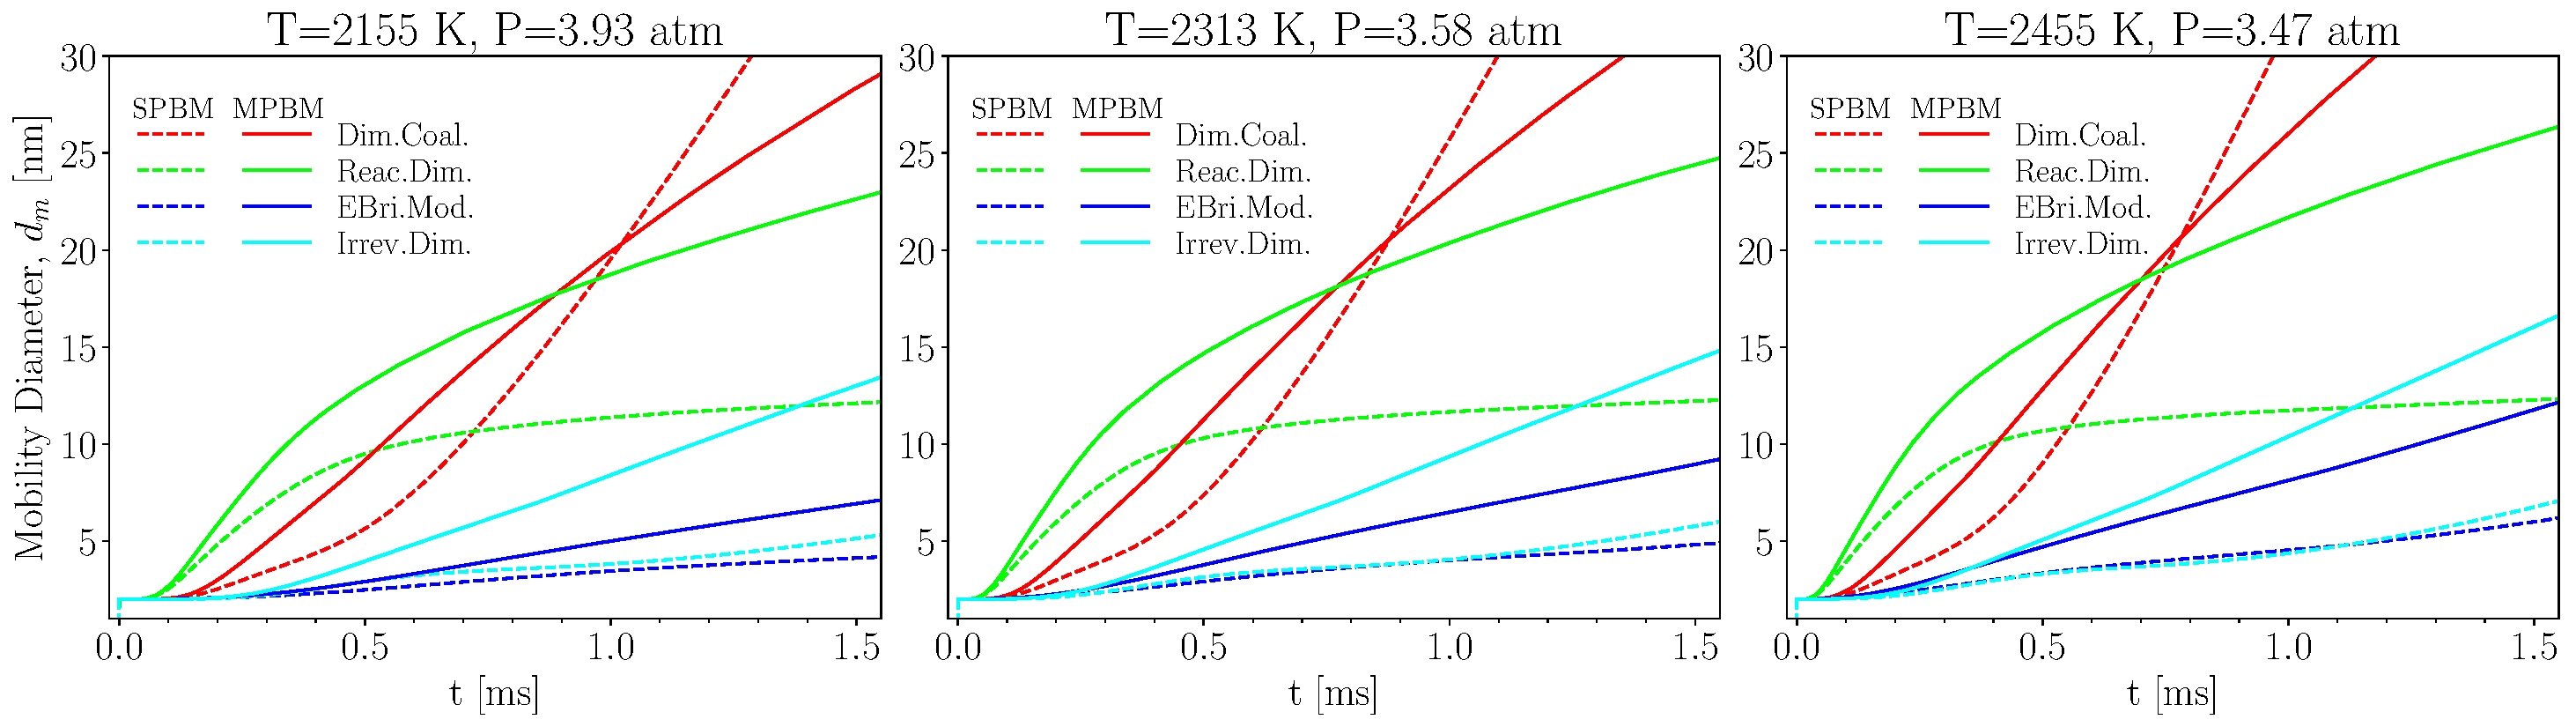
\includegraphics[width=1\textwidth]{Figures/Results/Shocktube/Stanford/june/30CH4_sootdm_kaust_subset.pdf}
	\caption{The time history of mobility diameter, $d_m$ of 30\% $\mathrm{CH_4}$ pyrolysis for T=2155, 2313, and 2455 K using KAUST with different combinations of PAH growth and particle dynamics models}
	\label{fig:shocktubest_30ch4_dm_kaust_subset} 
\end{figure}

As shown Fig.~\ref{fig:shocktubest_30ch4_dm_kaust_subset},  $d_m$ exhibits a stronger sensitivity to the employed particle dynamics model compared to $d_p$ because MPBM cannot capture the initial transition of particle population before the attainment of self-preserving size distribution. As a result, morphology (quantified by characteristic diameters) predicted by MPBM diverges from the SPBM results that are closer to actual polydisperse morphology of soot. Overall, Dimer Coalescence predicts a larger mean mobility diameter because of stronger inception flux at the beginning of simulation time (see Fig.~\ref{fig:shocktubest_30ch4_Iinc_kaust_subset}) leading to more primary particles and higher coagulation rate that generates larger agglomerates. Fig.~\ref{fig:shocktubest_30ch4_Ctot_kaust_single} shows the carbon addition rate by PAH adsorption is comparable and greater than that of HACA. This difference is more pronounced for Reactive Dimerization where PAH adsorption is larger by more than one order of magnitude. 

\begin{figure}[H]
	\centering
	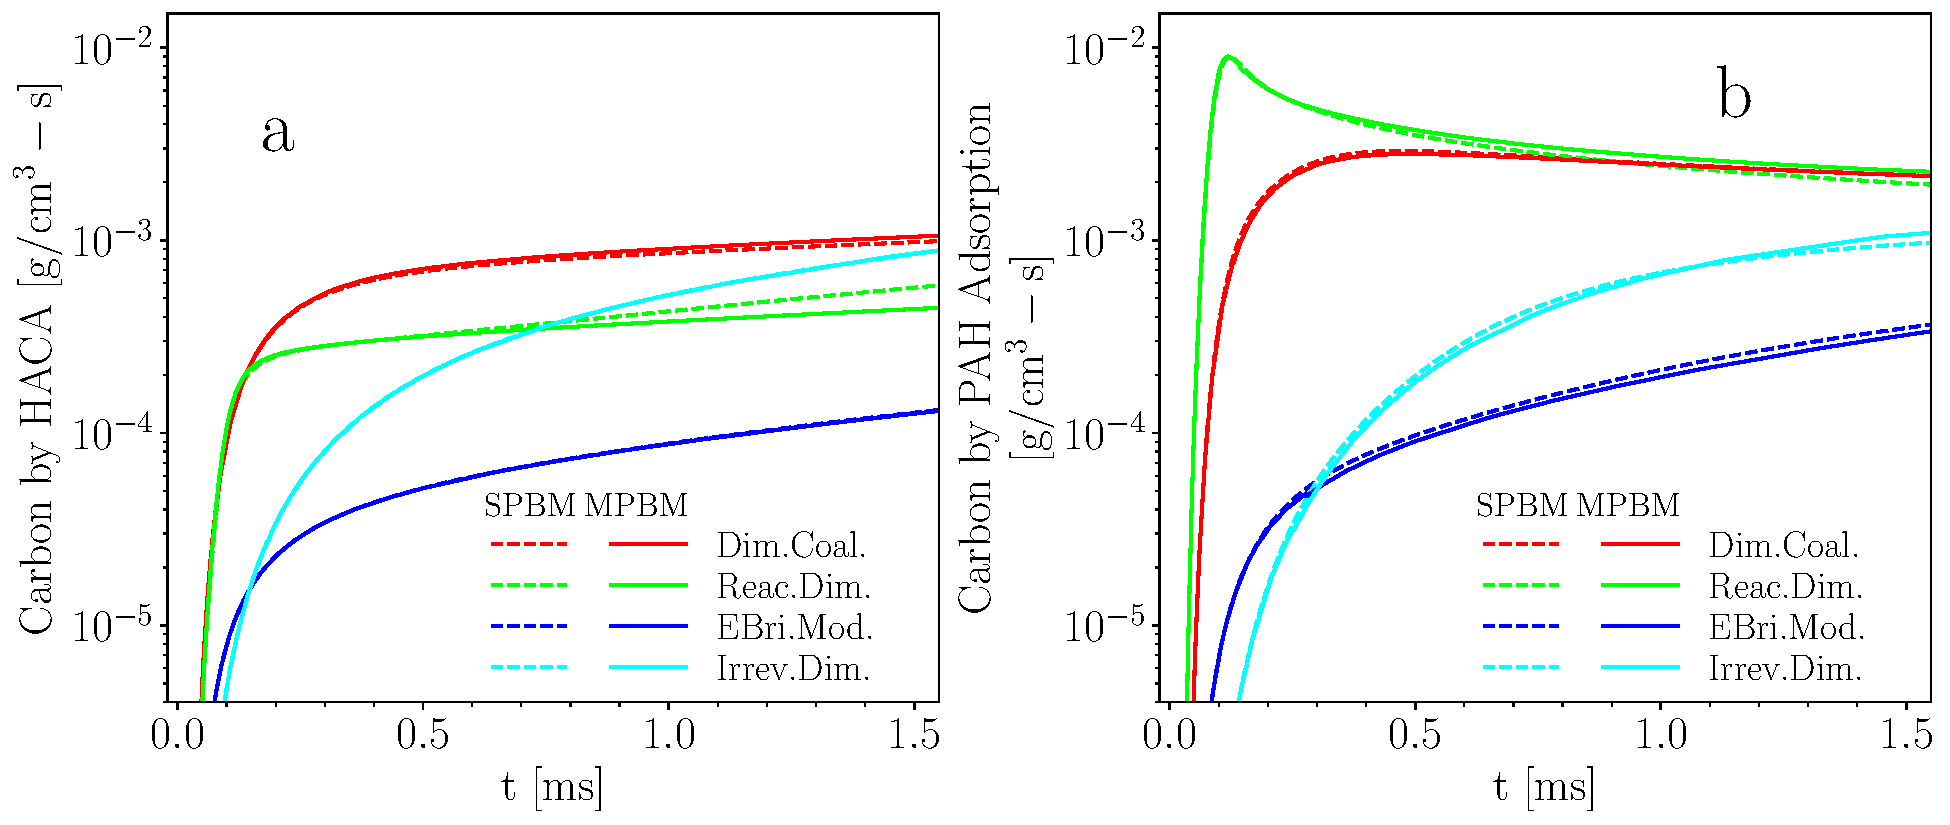
\includegraphics[width=0.67\textwidth]{Figures/Results/Shocktube/Stanford/june/30CH4_sootCtot_kaust_single.pdf}
	\caption{The time history of rate of carbon mass addition by (a) HACA and (b) PAH adsorption at T=2313 K using KAUST with different combinations of PAH growth and particle dynamics models}
	\label{fig:shocktubest_30ch4_Ctot_kaust_single} 
\end{figure}



%----------------------------------------------------------------
%
% STANFORD SHOKCTUBE DATA 10% CH4
%
%---------------------------------------------------------------

\subsection{10\% Methane Data-set}

The second data set from Stanford's group includes the measurements on 10\% $\mathrm{CH_4}$ pyrolysis at P=1$\pm$0.5 atm and 4$\pm$0.5 atm in the temperature range of 1800-2500 K. The first step is the examination of chemistry by comparing the predicted species mole fraction using different reaction mechanisms with data from laser diagnostics. Then, we look into soot volume fraction and morphology for a single data point at which TEM measurements were conducted, analyze the collected TEM images, identify main factors contributing to the discrepancies in volume fraction and morphology, optimize the PAH growth models to minimize the prediction error, and apply optimized model to the rest of data points. We limit our discussion to the 4-atm cases as extinction measurements showed negligible soot in 1-atm cases. The results of whole pressure and temperature ranges can be found in Section~\ref{sec:app_st_10CH4}.  

\subsubsection{Reaction Mechanism Assessment}
As shown in Fig.~\ref{fig:shocktubest_10ch4_ch4_nosoot_subset}, similar to 30\% dataset, KAUST yields the highest $\mathrm{CH_4}$ conversion followed by Caltech and ABF mechanism. While KAUST accurately predicts $\mathrm{CH_4}$ mole fraction over the studied temperature range, Caltech and ABF overpredict it indicating that less carbon is directed toward intermediates and larger hydrocarbons.

\begin{table}[]
	\caption{The pressure, temperature and composition of simulation data points for 10\% $\mathrm{CH_4}$}
	\centering
	\begin{tabular}{l|llllllllll|}
		\cline{2-11}
		& \multicolumn{10}{c|}{Datapoints}                       \\ \cline{2-11} 
		& (1)  & (2)  & (3)  & (4)  & (5)  & (6)  & (7)  & (8) & (9) & (10)  \\ \hline
		\multicolumn{1}{|l|}{T {[}K{]}} & 1873  & 1927 & 2074 & 2030 & 2348 & 1776 & 1897 & 2085 & 2277 & 2406 \\ \hline
		\multicolumn{1}{|l|}{P {[}atm{]}} & 1.09 & 1.37 & 1.27 & 1.22 & 1.13 & 4.76 & 4.49 & 4.85 & 4.43 & 3.89 \\ \hline
		\multicolumn{1}{|l|}{Composition} & \multicolumn{10}{c|}{$\mathrm{CH_4}$: 0.1, $\mathrm{CO_2}$: 0.01, Ar: 0.7}               \\ \hline
	\end{tabular}
	\label{tab:shocktubest_CH4_10} 
\end{table}

Fig.~\ref{fig:shocktubest_10ch4_c2h4_nosoot_subset} shows that ABF predicts the initial jump and gradual decrease towards equilibrium $\mathrm{C_2H_4}$ mole fraction at T=1897 K in good agreement with the data, but underpredicts it at higher temperatures. KAUST mechanism overpredicts $\mathrm{C_2H_4}$ production at the beginning leading to higher peak as well as its later consumption resulting in lower mole fraction towards the end of simulation compared to the measurements. Fig.~\ref{fig:shocktubest_10ch4_c2h2_nosoot_subset} depicts underprediction of $\mathrm{C_2H_2}$ mole fraction by all mechanisms over the whole temperature range, which is more pronounced for KAUST mechanism. Fig.~\ref{fig:shocktubest_10ch4_ccc_nosoot_subset} shows that carbon mass fraction in measured species decreases for all mechanisms showing conversion of carbon from major species to larger hydrocarbons, but similar to 30\% simulation, ABF predicts an increase in total carbon mass fraction. As shown in Fig.\ref{fig:shocktubest_10ch4_spc_nosoot_subset}, the carbon mass fraction of designated soot precursors predicted by ABF are lower by more than one order of magnitude compared to KAUST and Caltech.

\begin{figure}[H]
	\centering
	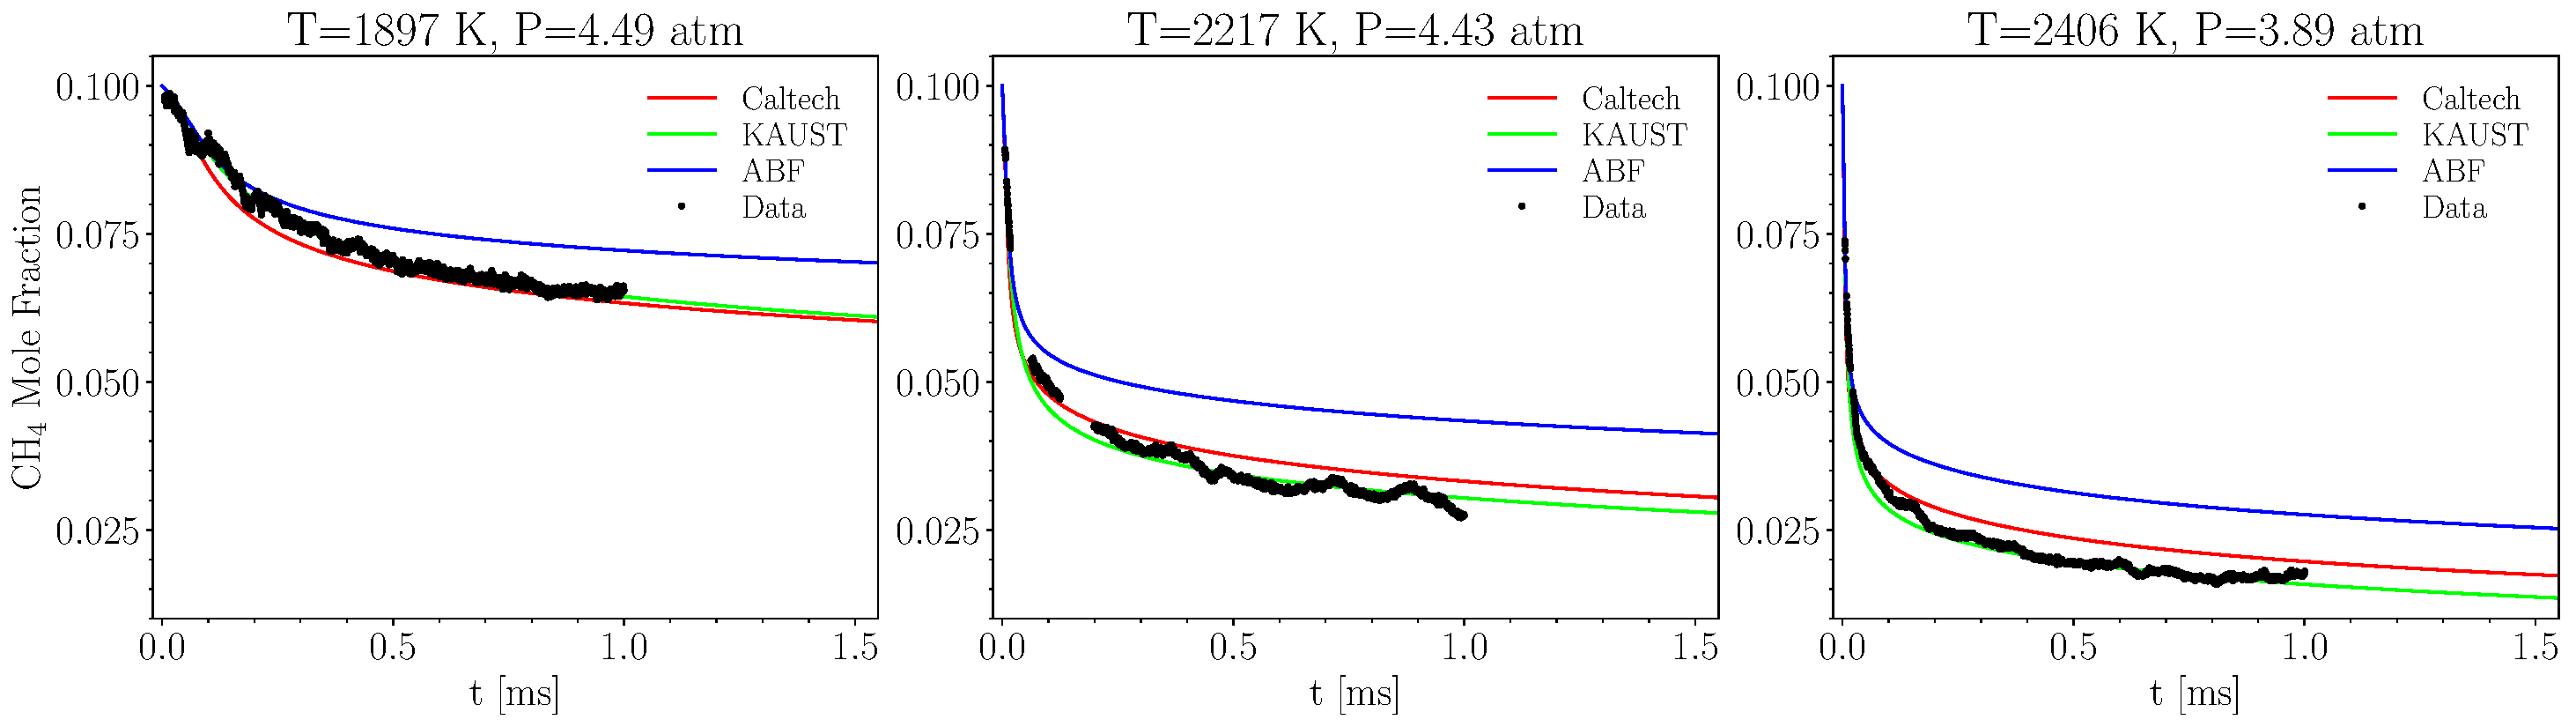
\includegraphics[width=1\textwidth]{Figures/Results/Shocktube/Stanford/September/10CH4_CH4_mechs_nosoot_subset.pdf}
	\caption{The time history of mole fraction of $\mathrm{CH_4}$ of 10\% $\mathrm{CH_4}$ pyrolysis at T=1897, 2217, and 2406 K using Caltech, KAUST, and ABF mechanisms compared with laser diagnostics data}
	\label{fig:shocktubest_10ch4_ch4_nosoot_subset} 
\end{figure}


 \begin{figure}[H]
	\centering
	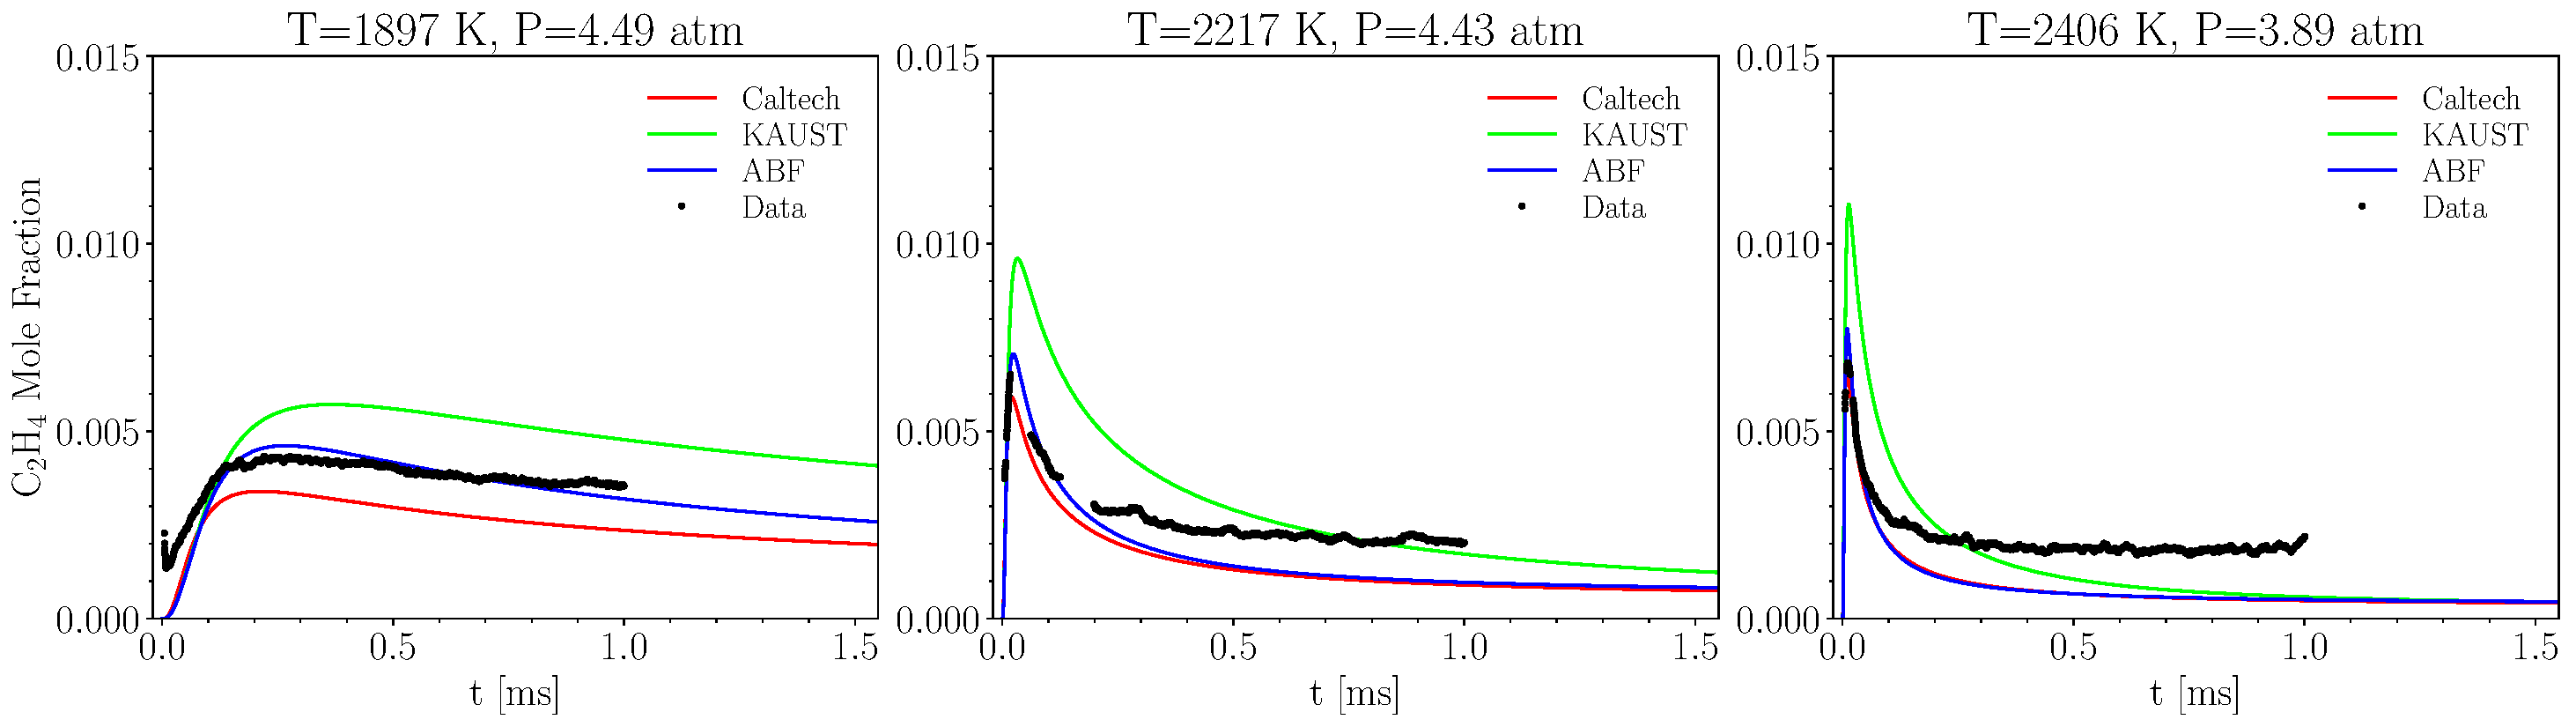
\includegraphics[width=1\textwidth]{Figures/Results/Shocktube/Stanford/September/10CH4_C2H4_mechs_nosoot_subset.pdf}
	\caption{The time history of mole fraction of $\mathrm{C_2H_4}$ of 10\% $\mathrm{CH_4}$ pyrolysis at T=1897, 2217, and 2406 K using Caltech, KAUST, and ABF mechanisms compared with laser diagnostics data}
	\label{fig:shocktubest_10ch4_c2h4_nosoot_subset} 
\end{figure}

\begin{figure}[H]
	\centering
	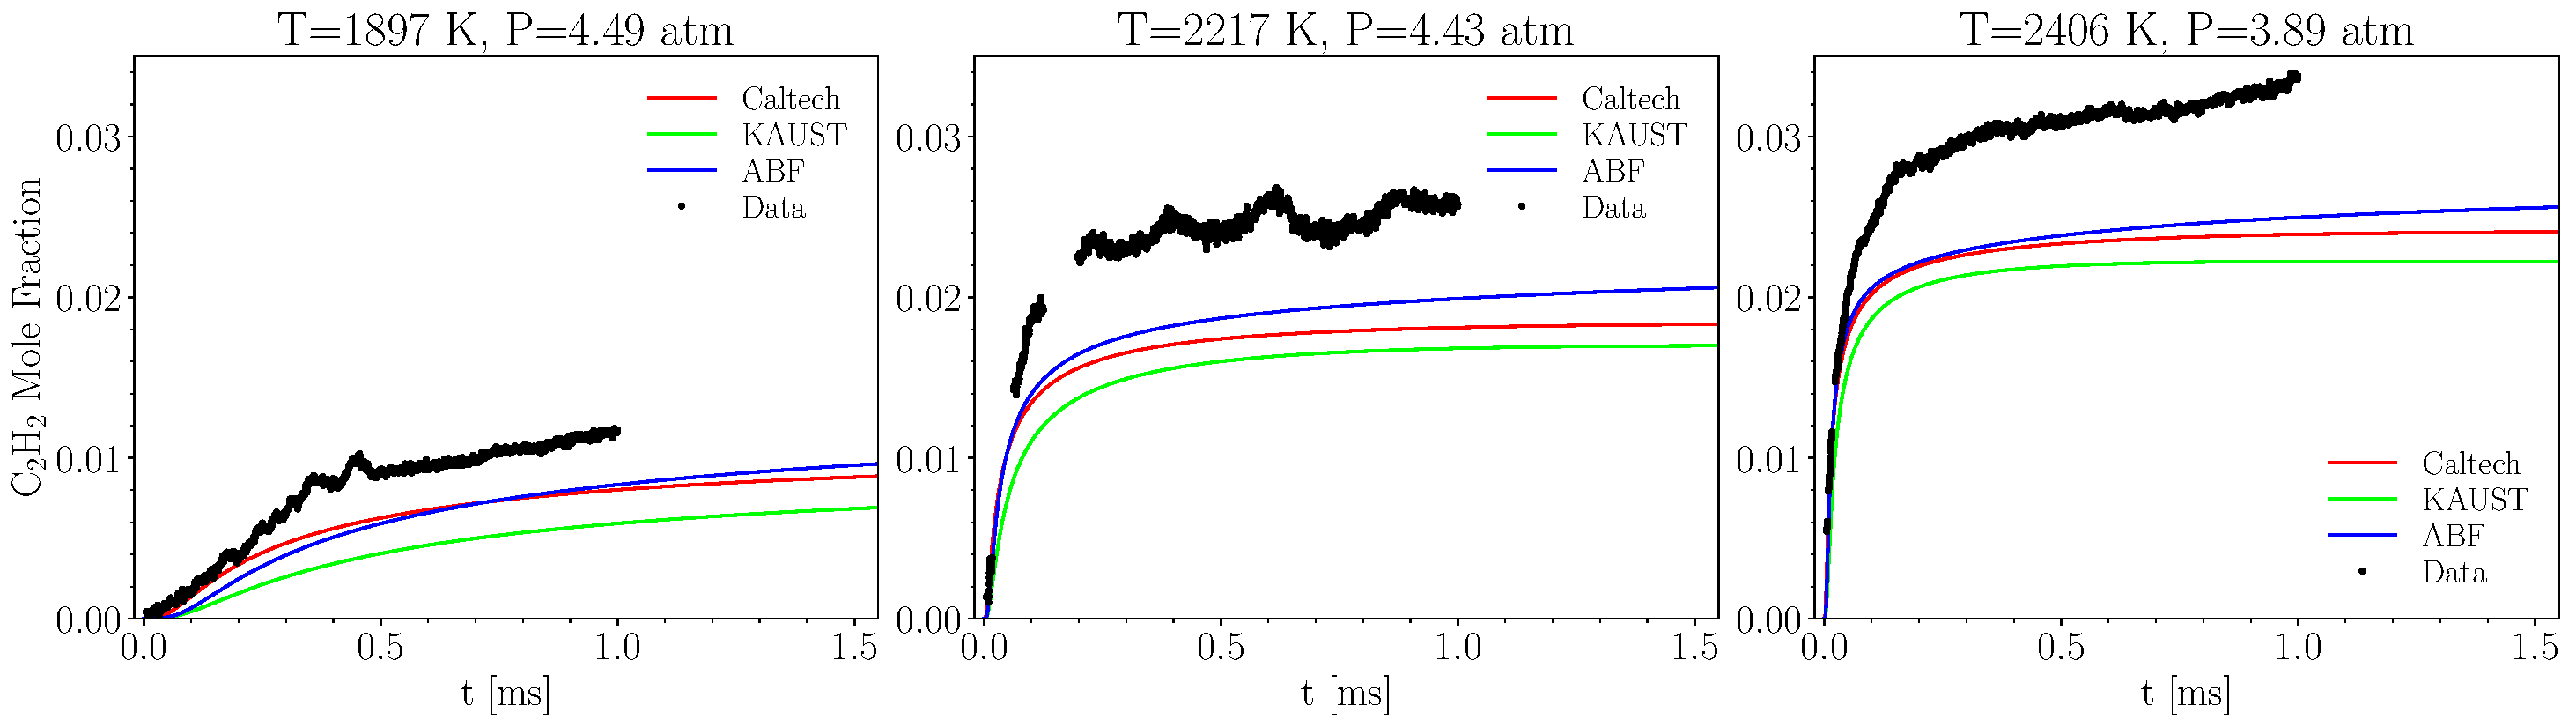
\includegraphics[width=1\textwidth]{Figures/Results/Shocktube/Stanford/September/10CH4_C2H2_mechs_nosoot_subset.pdf}
	\caption{The time history of mole fraction of $\mathrm{C_2H_2}$ of 10\% $\mathrm{CH_4}$ pyrolysis at T=1897, 2217, and 2406 K using Caltech, KAUST, and ABF mechanisms compared with laser diagnostics data}
	\label{fig:shocktubest_10ch4_c2h2_nosoot_subset} 
\end{figure}

\begin{figure}[H]
	\centering
	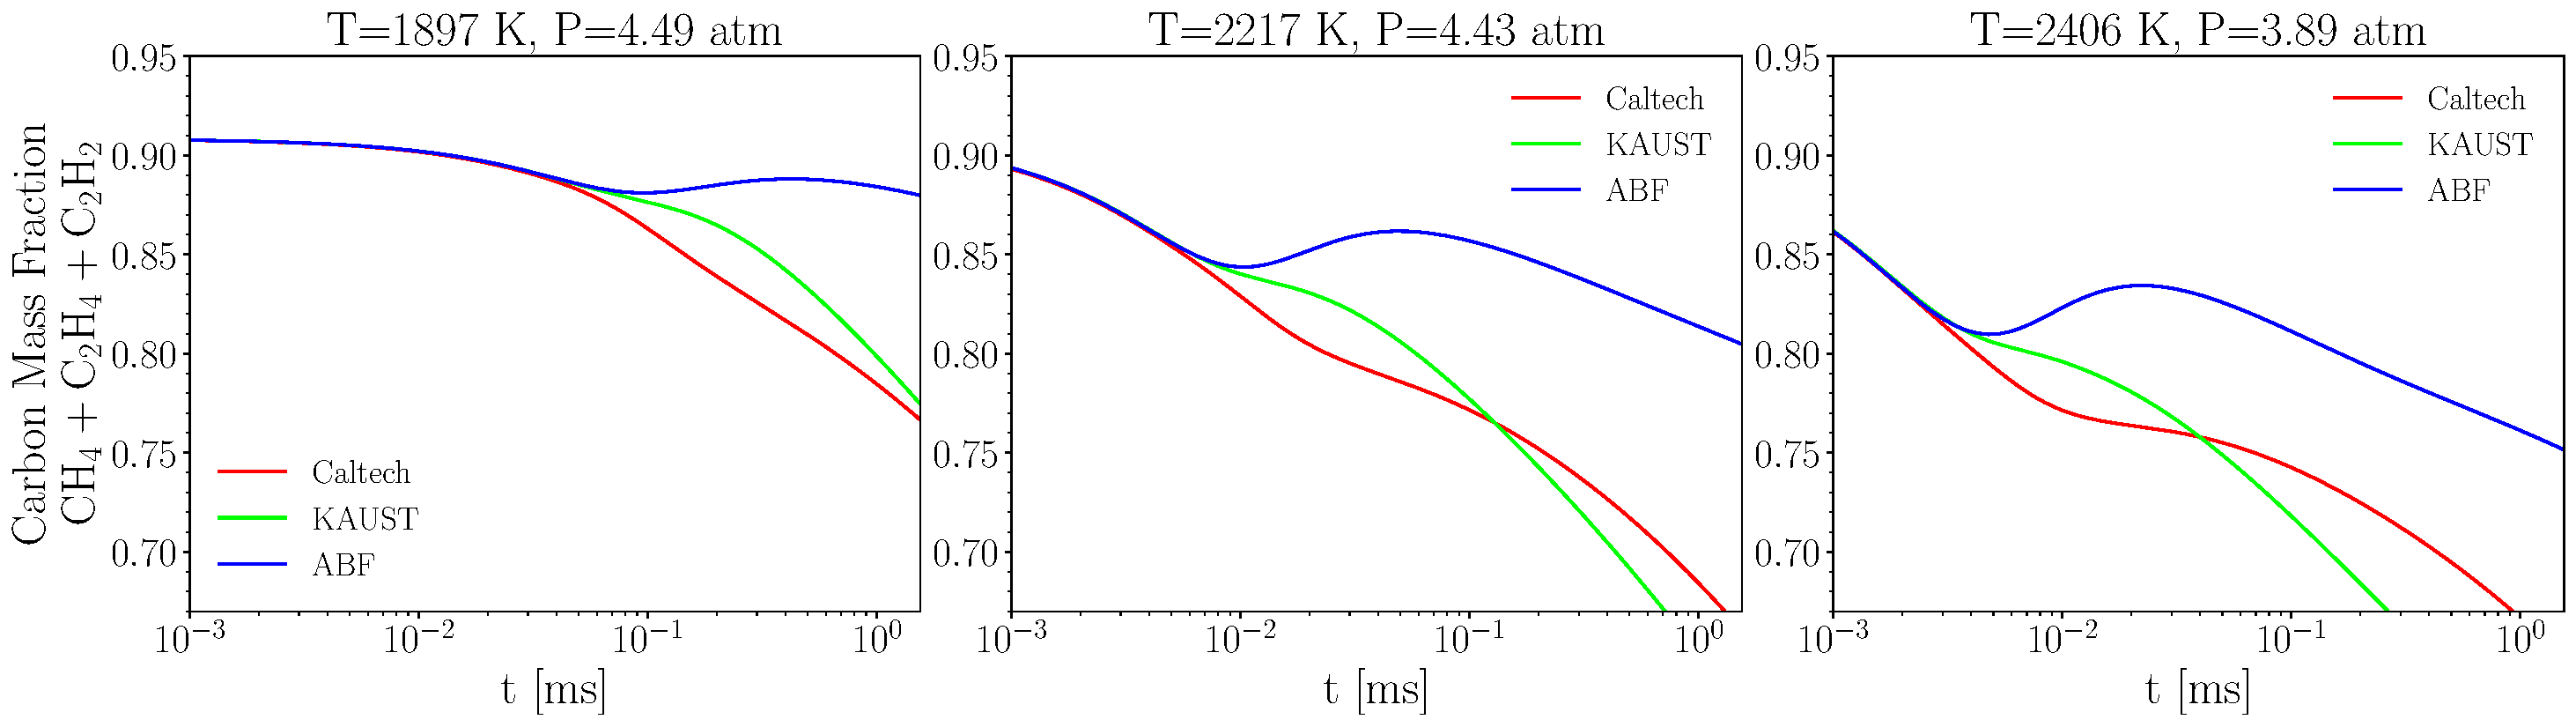
\includegraphics[width=1\textwidth]{Figures/Results/Shocktube/Stanford/September/10CH4_CCC_mechs_nosoot_subset.pdf}
	\caption{The time history of carbon mass fraction of $\mathrm{CH_4}$ $\mathrm{C_2H_4}$, $\mathrm{C_2H_2}$ of 10\% $\mathrm{CH_4}$ pyrolysis at T=1897, 2217, and 2406 K using Caltech, KAUST, and ABF mechanisms compared with laser diagnostics data}
	\label{fig:shocktubest_10ch4_ccc_nosoot_subset} 
\end{figure}


\begin{figure}[H]
	\centering
	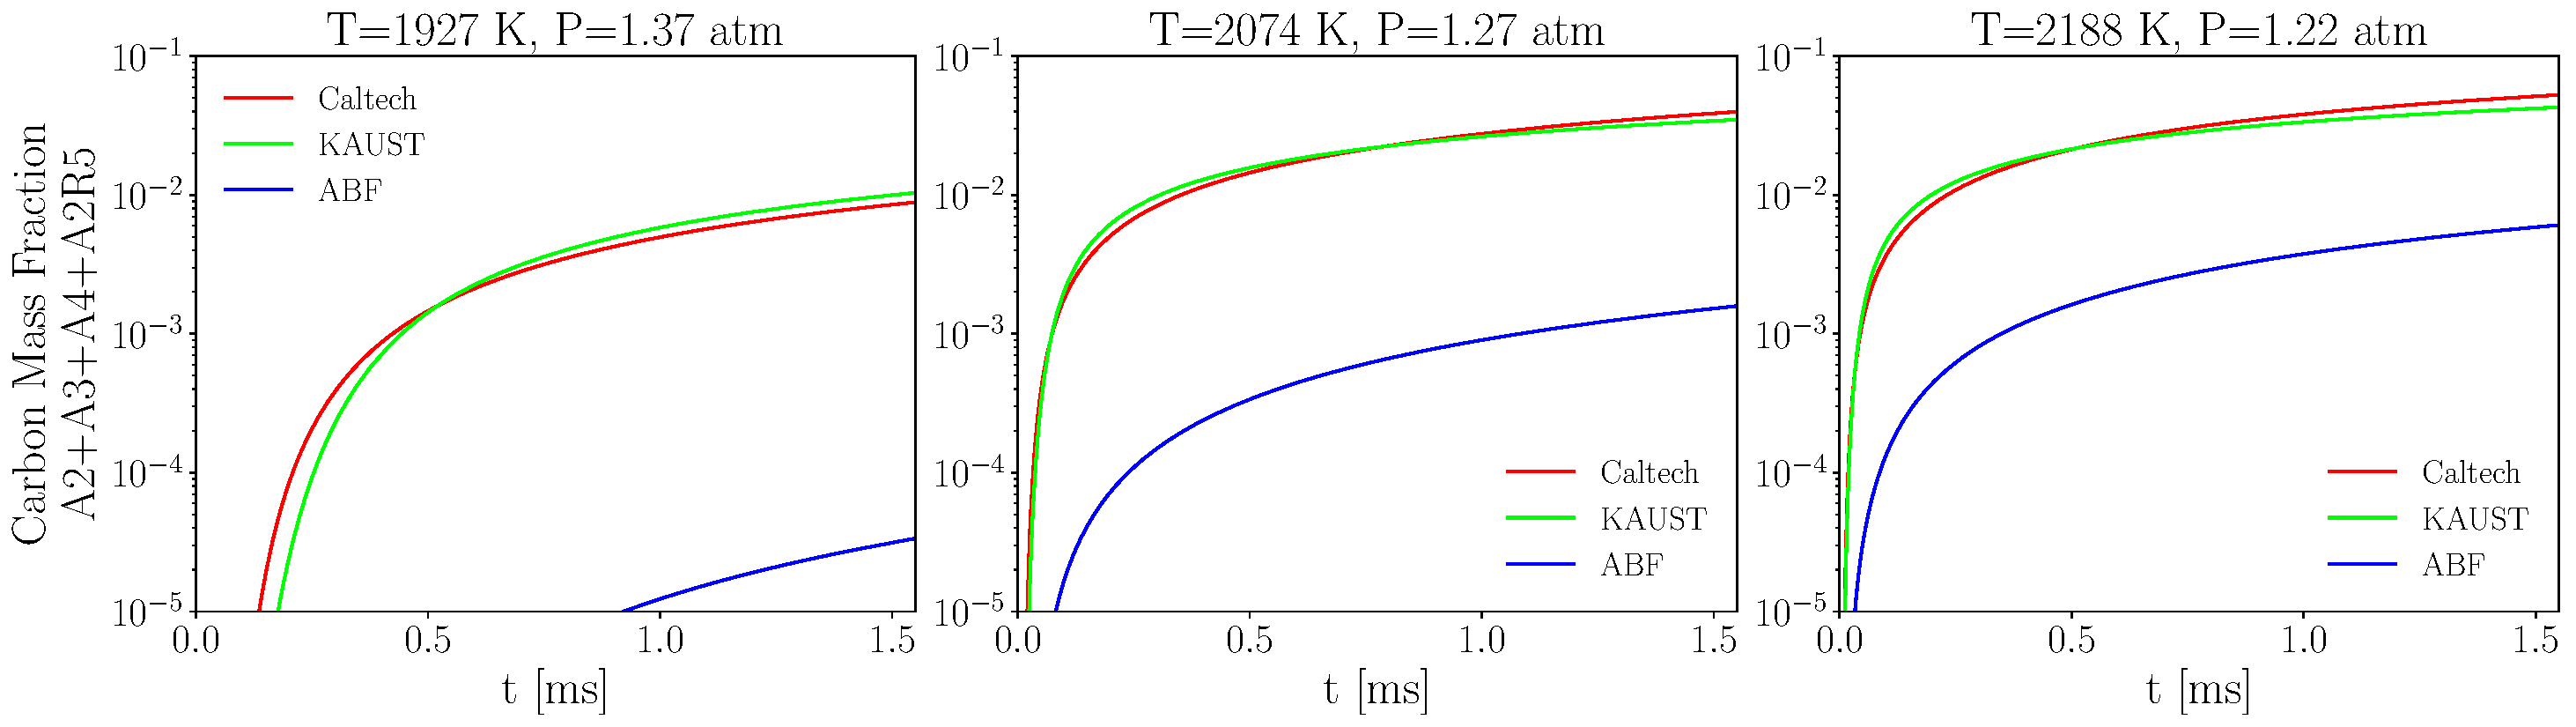
\includegraphics[width=1\textwidth]{Figures/Results/Shocktube/Stanford/September/10CH4_SPC_mechs_nosoot_subset.pdf}
	\caption{The time history of carbon mass fraction of A2, A3, A4, A2R5 of 10\% $\mathrm{CH_4}$ pyrolysis at T=1897, 2217, and 2406 K using Caltech, KAUST, and ABF mechanisms compared with laser diagnostics data}
	\label{fig:shocktubest_10ch4_spc_nosoot_subset} 
\end{figure}

%First, the mechanism comparison is conducted by simulating 10\% $\mathrm{CH_4}$ pyrolysis in a constant volume reactor. As shown before in Figs.~\ref{fig:shocktubestch4} and ~\ref{fig:shocktubestc2h2}, the particle dynamics and PAH growth models has minimal effect on the prediction of major small hydrocarbons. So, the mechanism comparison is only based on the combination of MPBM and RD to avoid clutter in graphs, and it is focused on two data points, T=2188 K, P=1.22 atm and T=2217 K, P=4.43 atm, each being representative of atmospheric and high pressure cases, respectively. Fig.\ref{fig:shocktubes_sepch4} shows $\mathrm{CH_4}$ mole fraction for these data points predicted using KAUST, Caltech, and ABF mechanisms and compared with measurements. Similar to 30\% $\mathrm{CH_4}$ data set, KAUST and Caltech yield larger $\mathrm{CH_4}$ conversion corresponding to a lower mole fraction. However, KAUST predictions are in close agreement for both data points, but ABF underestimates $\mathrm{CH_4}$ conversion. As shown in Fig.~\ref{fig:shocktubes_sepc2h2}, all mechanisms exhibit a similar behavior underestimating $\mathrm{C_2H_2}$ mole fraction in the high pressure, but overestimating it for the atmospheric case. Fig.~\ref{fig:shocktubes_sepvf} compares soot volume fraction predicted by different mechanisms with light extinction measurements. As expected, ABF significantly underpredicts $f_v$ due to low production rate of soot precursors (PAHs). Temperature analysis is not done for 10\% $\mathrm{CH_4}$ due to lack of measurements. KAUST mechanism is used for soot analysis as it predicts species and soot volume fraction close to the measurements.
%
%\begin{figure}[H]
%	\centering
%	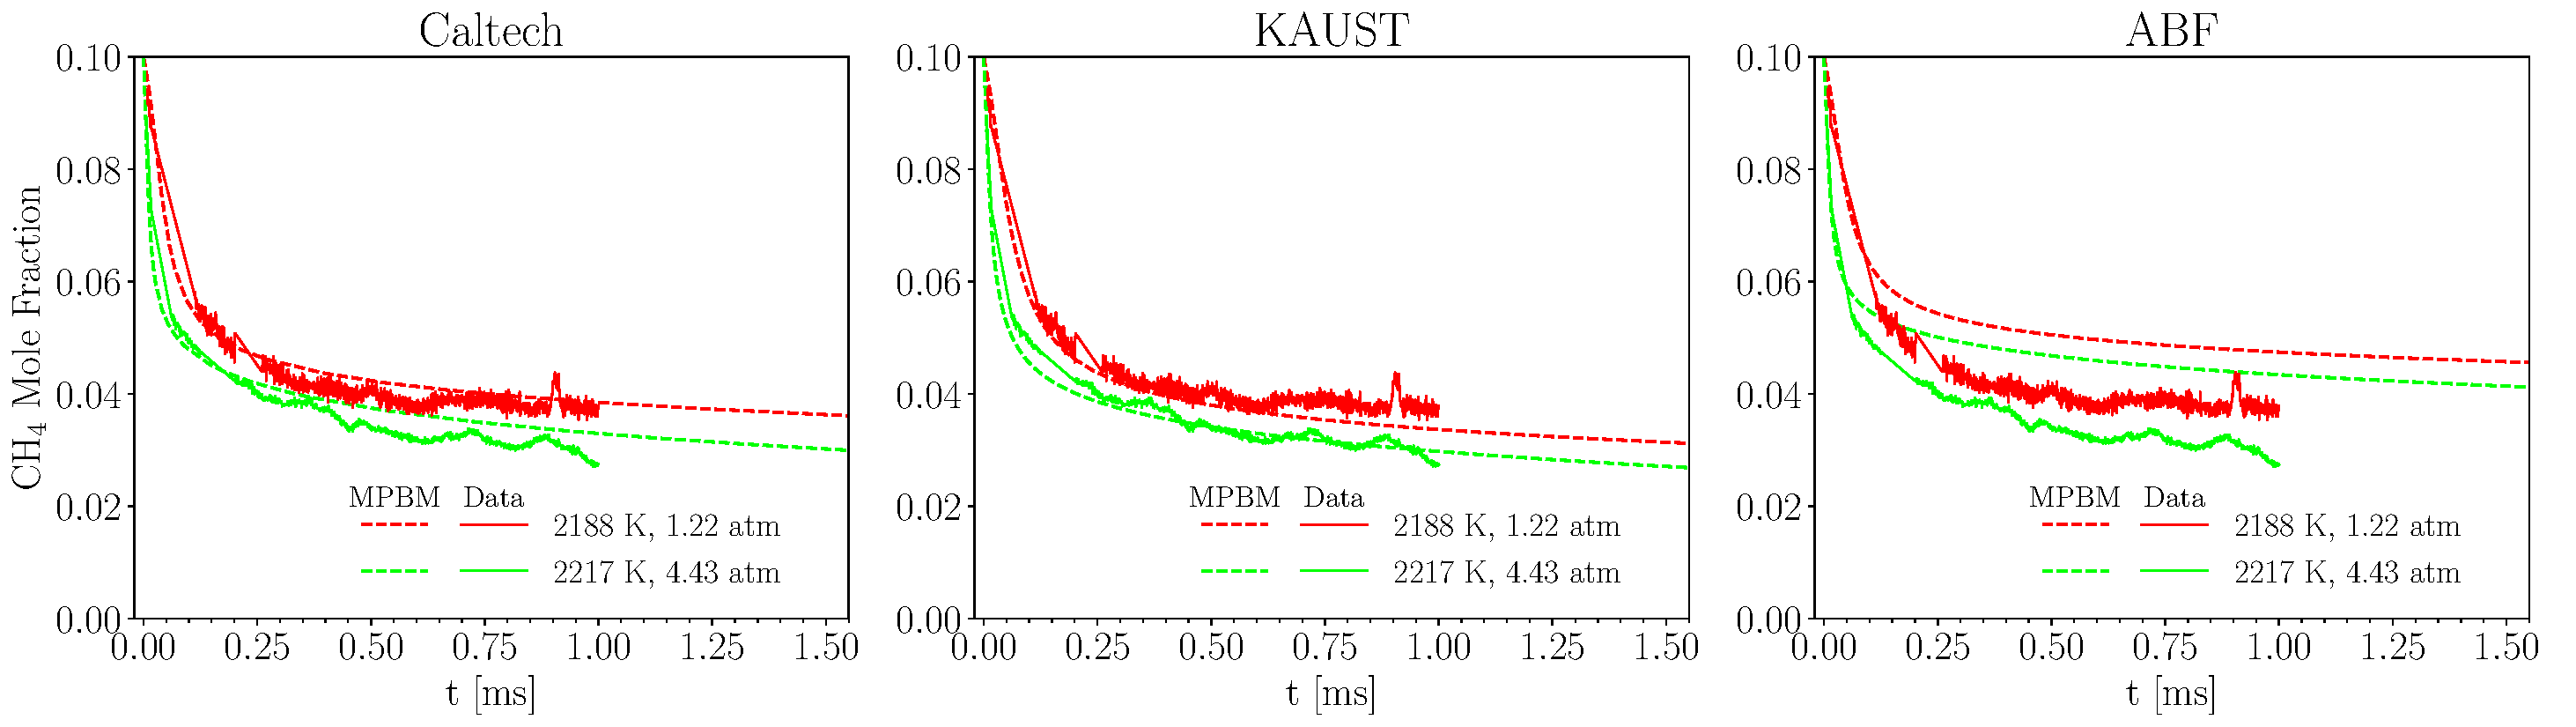
\includegraphics[width=1\textwidth]{Figures/Results/Shocktube/Stanford/September/stsh_sepmechs_CH4.pdf}
%	\caption{The time history of $\mathrm{CH_4}$ mole fraction during 10\% $\mathrm{CH_4}$ pyrolysis at T=2188 K, P=1.22 atm (red line) and T=2217 K, P=4.43 atm (green line) using Caltech, KAUST, and ABF mechanism with MPBM and Reactive Dimerization}
%	\label{fig:shocktubes_sepch4} 
%\end{figure}
%
%\begin{figure}[H]
%	\centering
%	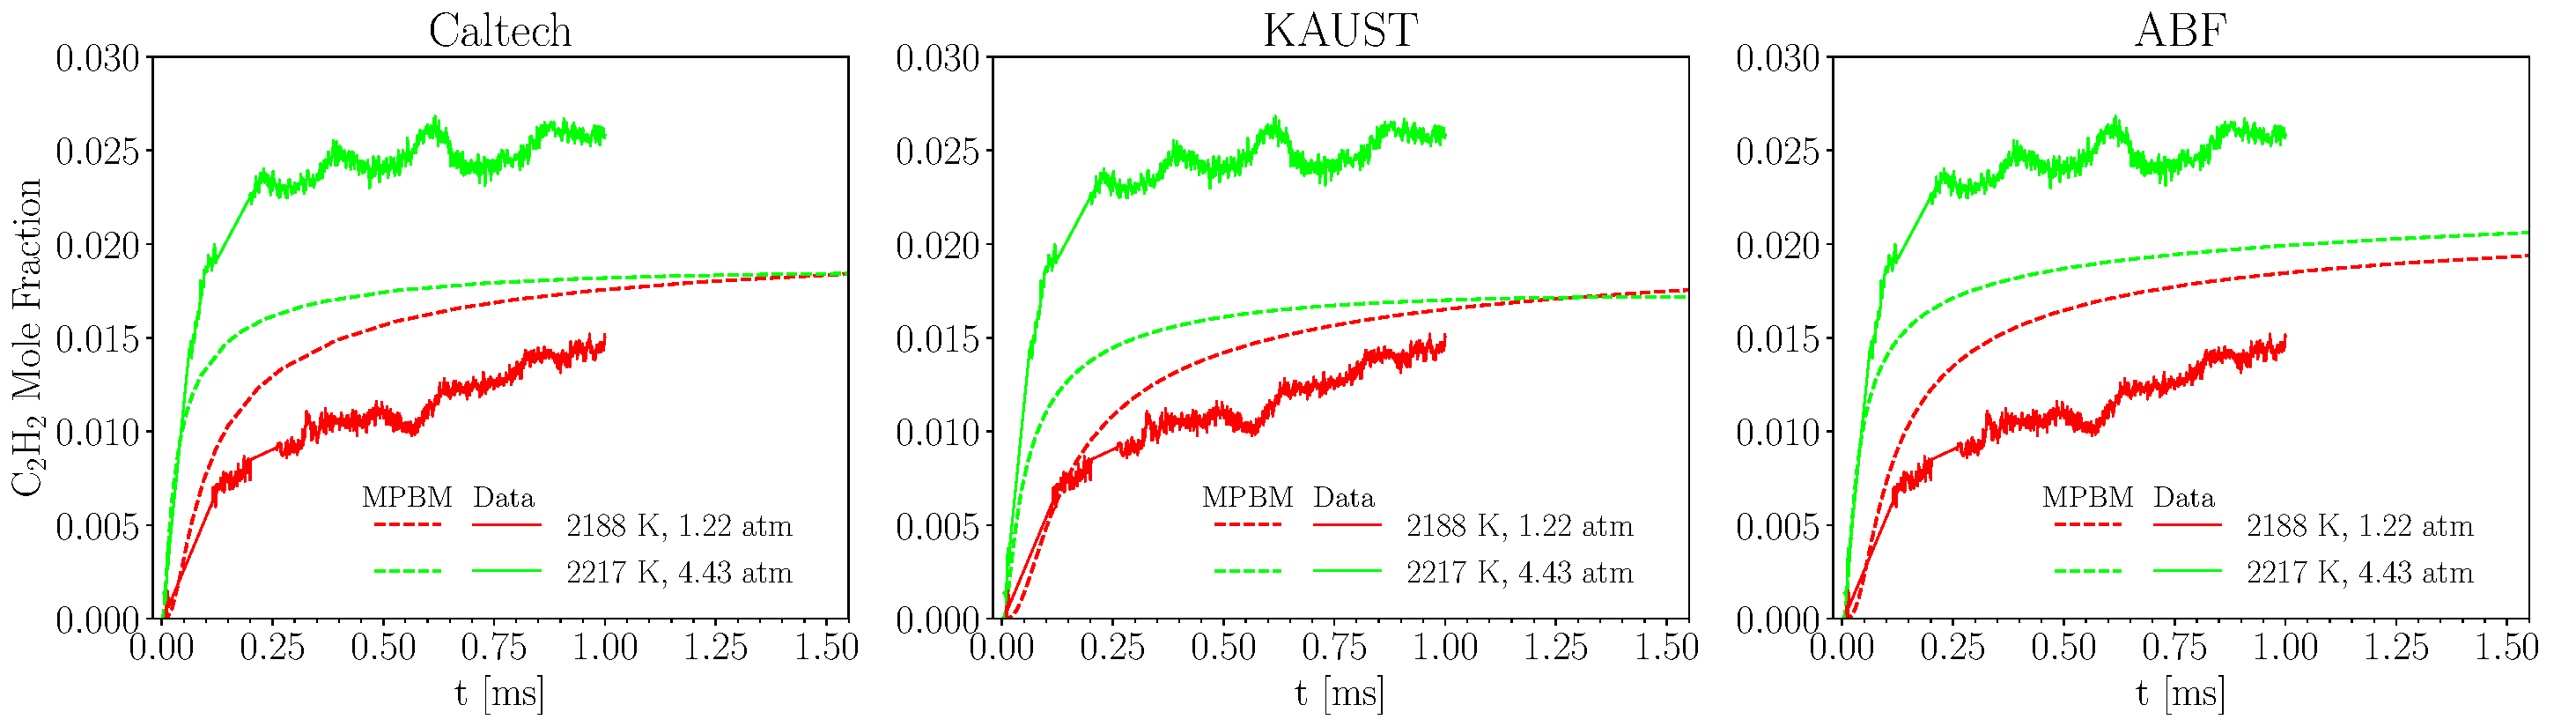
\includegraphics[width=0.9\textwidth]{Figures/Results/Shocktube/Stanford/September/stsh_sepmechs_C2H2.pdf}
%	\caption{The time history of $\mathrm{C_2H_2}$ mole fraction during 10\% $\mathrm{CH_4}$ pyrolysis at T=2188 K, P=1.22 atm (red line) and T=2217 K, P=4.43 atm (green line) using Caltech, KAUST, and ABF mechanism with MPBM and Reactive Dimerization}
%	\label{fig:shocktubes_sepc2h2} 
%\end{figure}
%
%\begin{figure}[H]
%	\centering
%	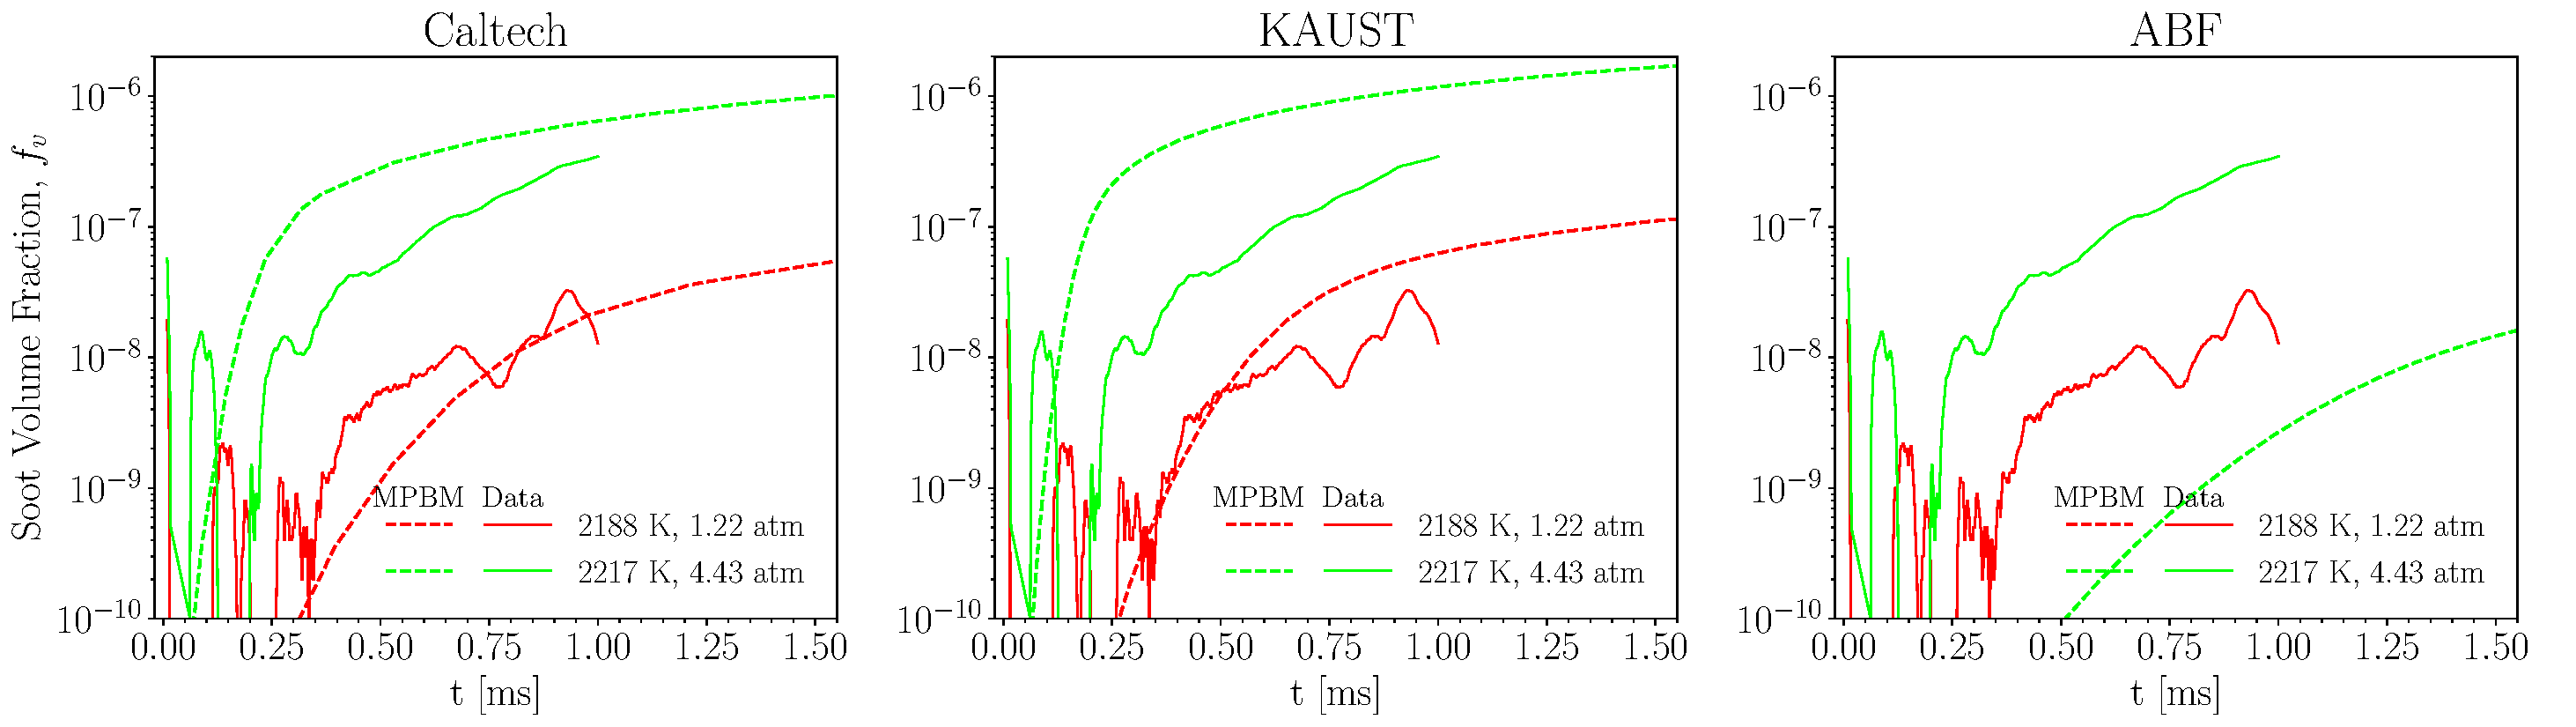
\includegraphics[width=0.9\textwidth]{Figures/Results/Shocktube/Stanford/September/stsh_sepmechs_vf.pdf}
%	\caption{The time history of soot volume fraction, $f_v$ of 10\% $\mathrm{CH_4}$ pyrolysis at T=2188 K, P=1.22 atm (red line) and T=2217 K, P=4.43 atm (green line) using Caltech, KAUST, and ABF mechanism with MPBM and Reactive Dimerization}
%	\label{fig:shocktubes_sepvf} 
%\end{figure}
%
%Fig.~\ref{fig:shocktubest_sepcasevf} shows the evolution of soot volume fraction, $f_v$ over simulation time in the temperature range (increasing from left to right) and (near) atmospheric and 4 atm pressure using KAUST mechanism. The upper and bottom rows correspond to 1 and 4 atm cases, and each column contains cases with similar temperatures. As expected, $f_v$ is not affected by particle dynamics model, but it increases with shock tube temperature. The time of $f_v=10^{-10}$ is shorter for 4 atm cases in each temperature indicating that pressure accelerates the soot formation. EF yields the most accurate $f_v$ prediction compared with the data in 2000-2500 K of 4 atm cases. The final $f_v$ predicted by increases by two orders of magnitude in 1900-2500 range at both pressures indicating more sensitivity of its inception rate to temperature.
%
%
%\begin{figure}[H]
%	\centering
%	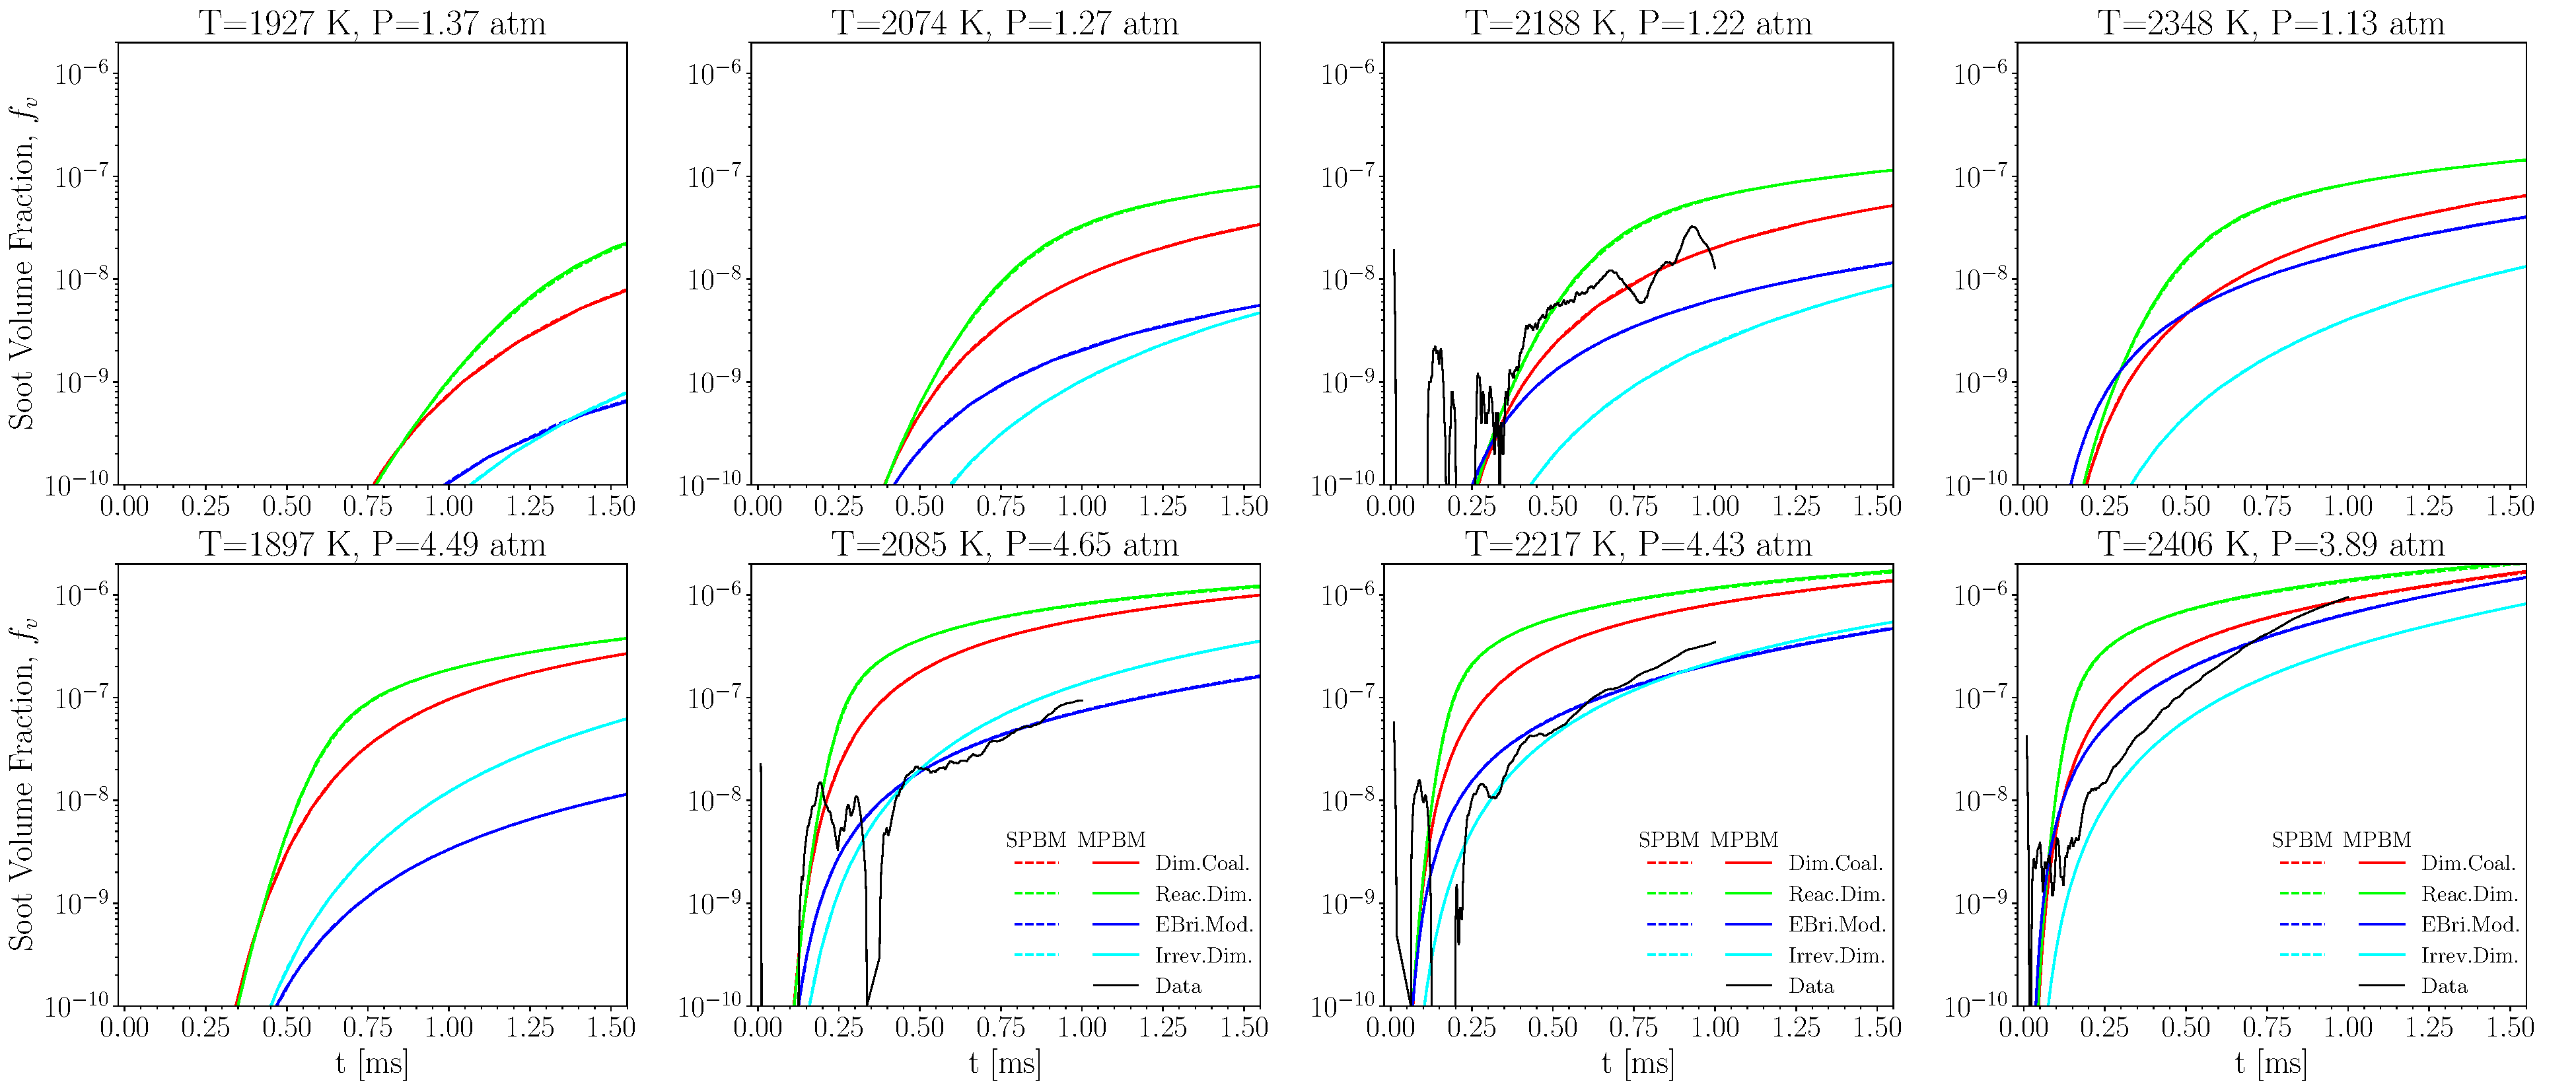
\includegraphics[width=1\textwidth]{Figures/Results/Shocktube/Stanford/September/stsh_cases_vf.pdf}
%	\caption{The time history of soot volume fraction of 10\% $\mathrm{CH_4}$ pyrolysis in the temperature range of 1900-2500 K (increasing from left to right) and P=1$\pm$0.5 (bottom row) and 4$\pm$0.5 atm (upper row) using KAUST mechanism and different PAH growth and particle dynamics models}
%	\label{fig:shocktubest_sepcasevf} 
%\end{figure}
%
%Figs.~\ref{fig:shocktubest_sepcasedp} and \ref{fig:shocktubest_sepcasedm} show time history of $d_p$ and $d_m$, respectively. The largest $d_p$ is predicted by RD in all cases with final values near 6 nm, which is close to $d_p$ of 10\% $\mathrm{CH_4}$. However, $d_m$ significantly decreased when feed-stock mole fraction is lowered from \%30 to \%10. Overall, the $d_p$ increases slightly with both temperature and pressure. RD has the largest $d_m$ in the entire temperature range of atmospheric cases, but at 4 atm $d_m$ by DC quickly increases and exceed RD due to stronger inception rate leading to larger coagulation rate and agglomerates. 
%
%\begin{figure}[H]
%	\centering
%	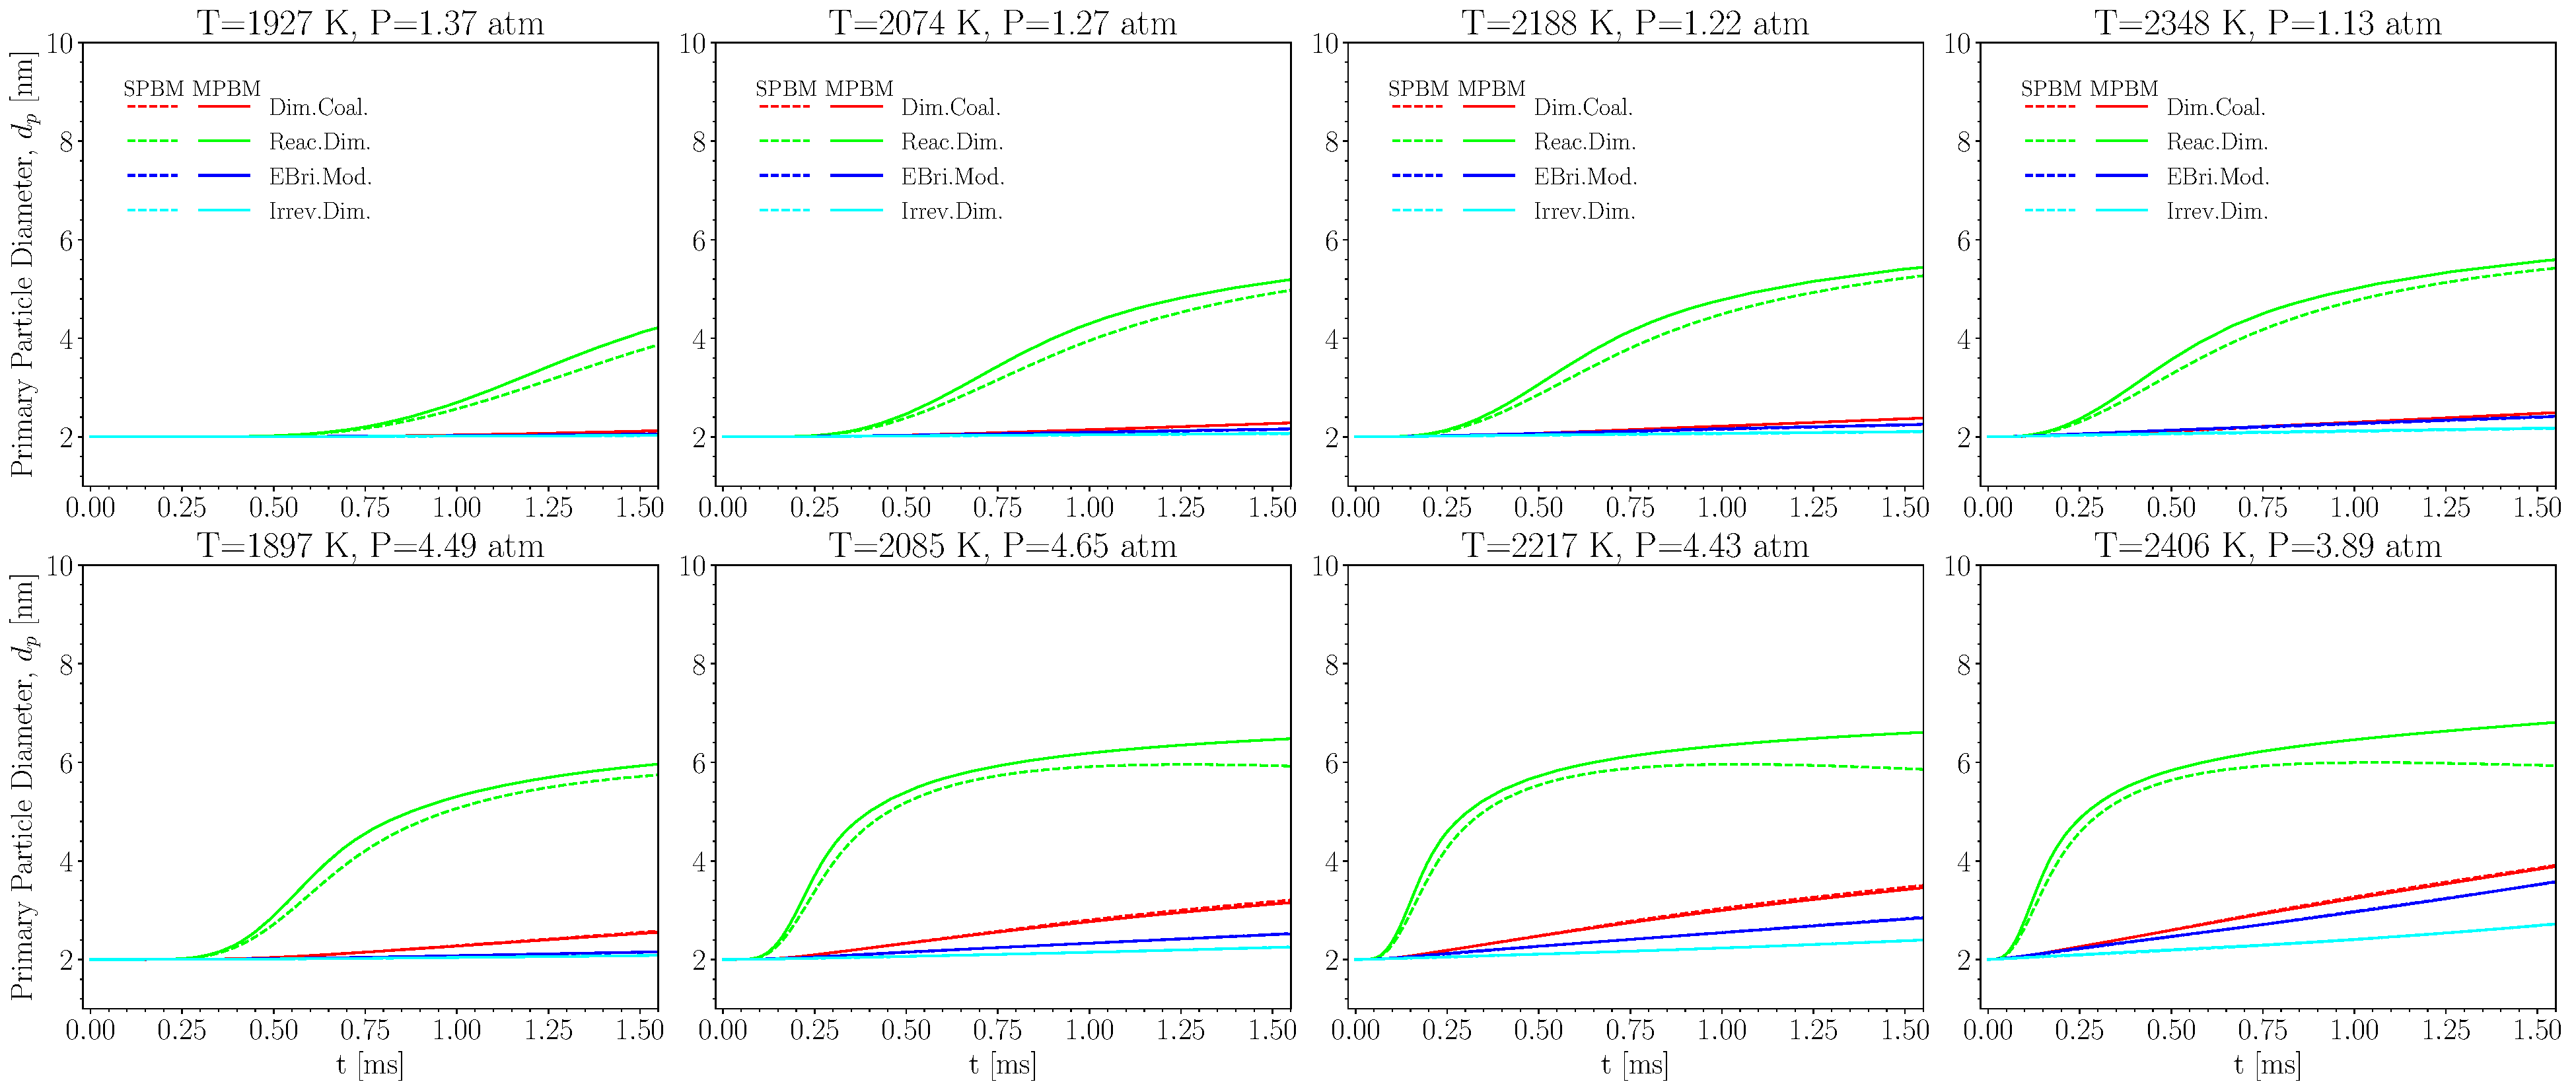
\includegraphics[width=1\textwidth]{Figures/Results/Shocktube/Stanford/june/stsh_cases_dp.pdf}
%	\caption{The time history of primary particle diameter, $d_p$ of 30\% $\mathrm{CH_4}$ pyrolysis in the temperature range of 1800-2500 K and P=1$\pm$0.5 and 4$\pm$0.5 atm using KAUST mechanism and different PAH growth and particle dynamics models}
%	\label{fig:shocktubest_sepcasedp} 
%\end{figure}
%
%\begin{figure}[H]
%	\centering
%	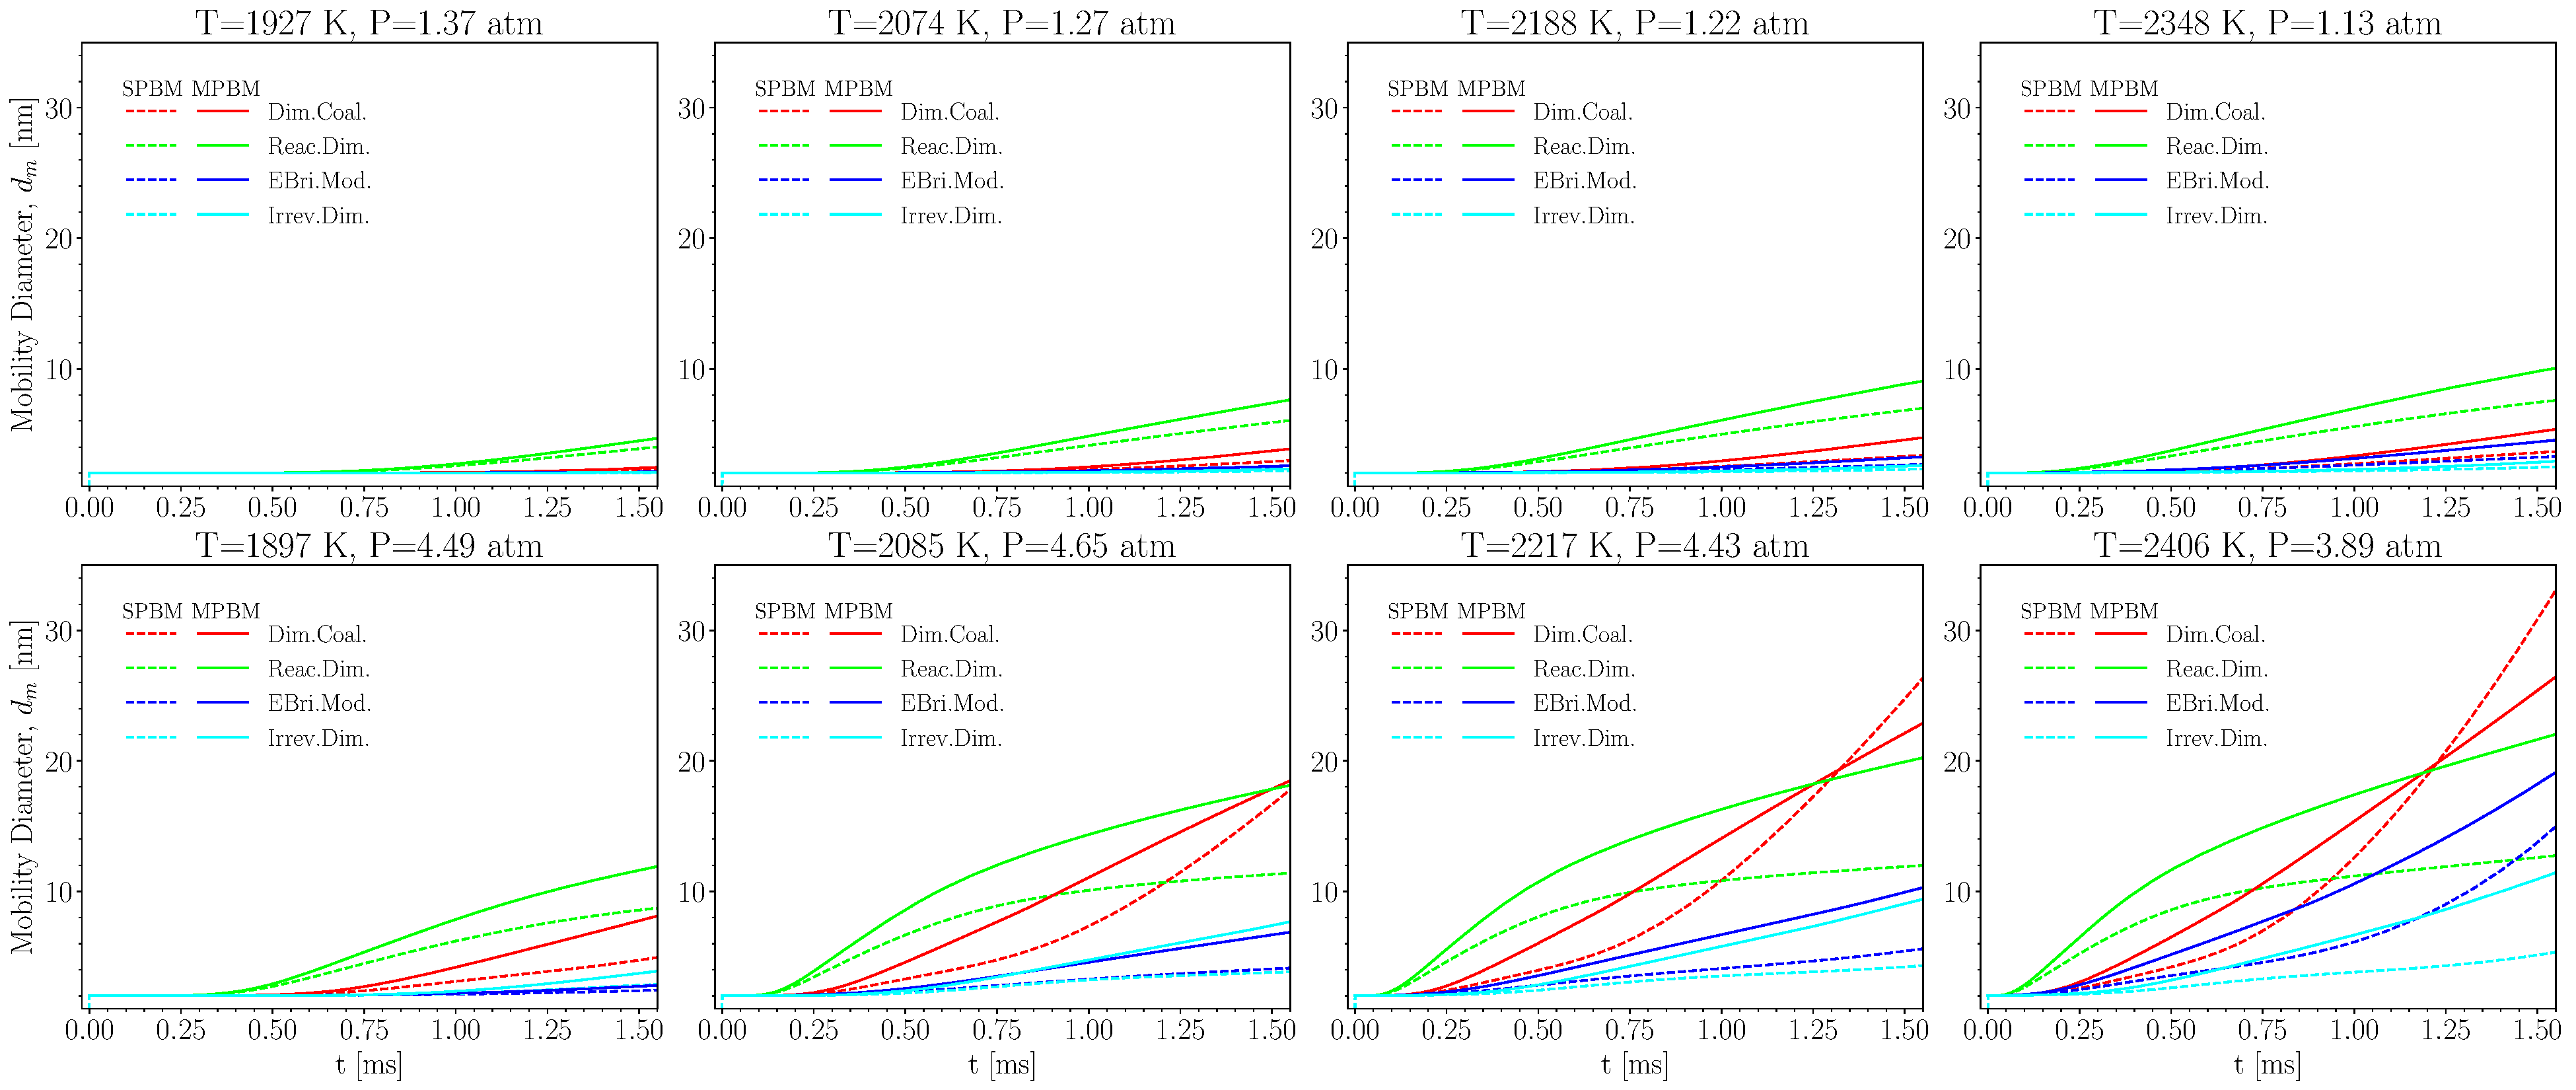
\includegraphics[width=1\textwidth]{Figures/Results/Shocktube/Stanford/September/stsh_cases_dm.pdf}
%	\caption{The time history of mobility diameter, $d_m$ of 30\% $\mathrm{CH_4}$ pyrolysis in the temperature range of 1800-2500 K and P=1$\pm$0.5 and 4$\pm$0.5 atm using KAUST mechanism and different PAH growth and particle dynamics models}
%	\label{fig:shocktubest_sepcasedm} 
%\end{figure}

\subsubsection{Characterization of soot morphology in methane pyrolysis shock-tube}

The TEM images of soot made during pyrolysis of 10\% $\mathrm{CH_4}$ was provided by Stanford group for a single data point of T=2217 K and P=4.5 atm that can be used to characterize soot morphology from ${d_p}$ and ${d_m}$. The images in addition to soot volume fraction enables assessing the performance of omnisoot in the description of soot generated during methane pyrolysis in the shock-tube. As reported by Stanford team, the expansion wave traverses the shock tube around 2 ms reducing the temperature to nearly 1000 K freezing the chemical reactions that contribute to the surface growth, but the coagulation continues until the collection of particles leading to larger agglomerates. As a result, $d_p$ estimated from the TEM images closely represents $d_p$ of agglomerates at the end of process, but $d_m$ estimated from TEM images could be larger than the actual values due to post-expansion-wave growth of particles. \textit{atems} package~\citep{sipkens2021using} was used for characterizing soot aggregates recorded in TEM images with different methods for evaluating the aggregate projected area, perimeter, and primary particle diameter. It creates a binary map from the raw TEM image where white and black pixels represent the agglomerates and background, respectively, and feeds the map to an agglomerate segmentation algorithm to detect individual agglomerates. Fig.\ref{fig:shocktubest_binarymapprocess} shows a sample from TEM images and segmented agglomerates from the generated map.

\begin{figure}[H]
	\centering
	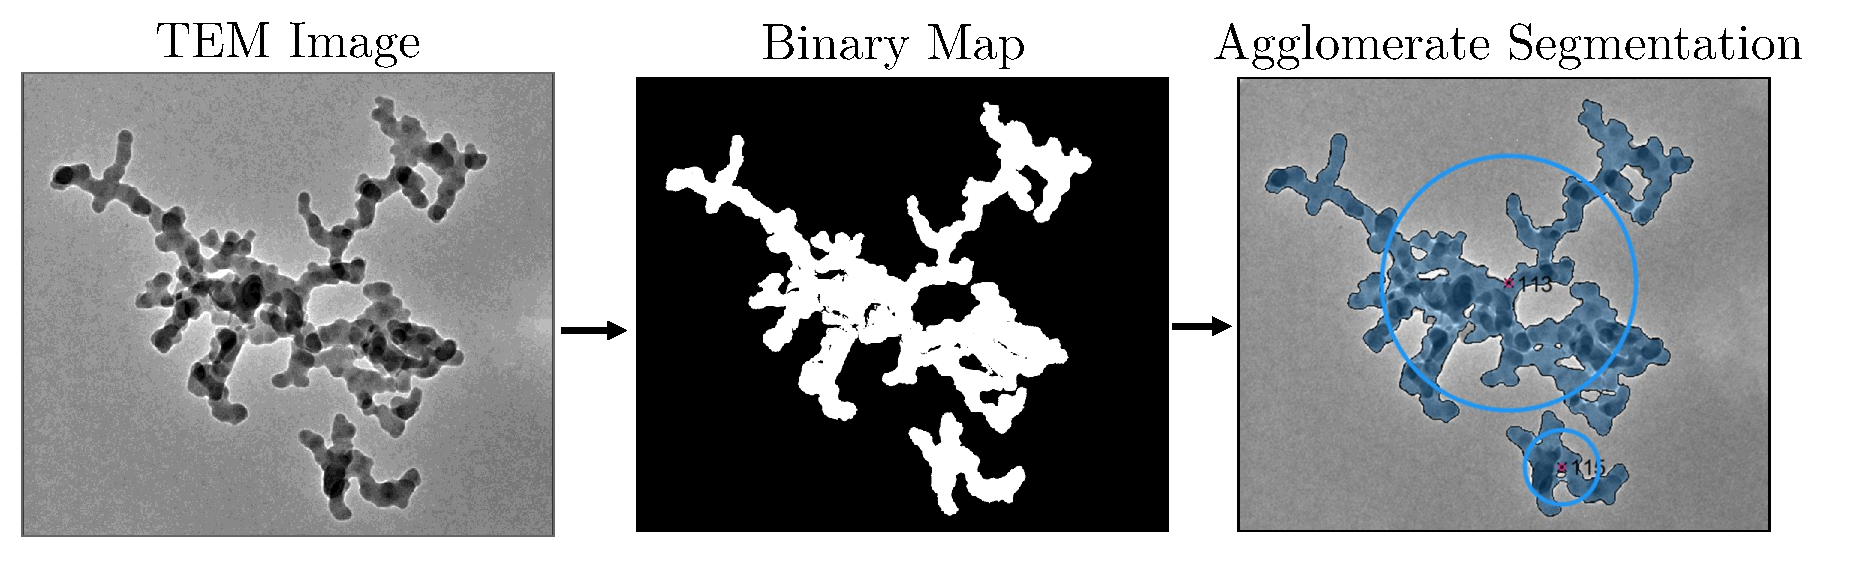
\includegraphics[width=0.9\textwidth]{Figures/Results/Shocktube/Stanford/TEM/binarymapprocess.pdf}
	\caption{A TEM image provided by Stanford group (left pane) with the generated binary map (middle pane) and detected agglomerates using the segmentation algorithm (right pane)}
	\label{fig:shocktubest_binarymapprocess} 
\end{figure}

We applied K-means clustering (KMC)~\citep{sipkens2021using} and otsu thresholding~\citep{dastanpour2016automated} to the same TEM images and compared the segmented agglomerates. A sample is shown in Fig.\ref{fig:shocktubest_aggseg_compare} where KMC detected more agglomerates in the TEM image, but segments part of the background as agglomerates or divides a single agglomerate into multiple ones. On the other hand, otsu thresholding misses most of agglomerates in the sampled TEM image. Here, the K-means clustering~\citep{sipkens2021using} is used and 171 agglomerates were detected. $d_m$ was calculated from the diameter of equivalent projected area , $A_a$ of each agglomerate. The pair correlation method (PCM)~\citep{dastanpour2016automated} was applied to compute the projected primary particle area, $A_p$ and the mean $d_p$ assuming that primary particle are almost uniform in size within each agglomerate. The arithmetic mean of $d_p$ of the entire samples is calculated as 

\begin{equation}
	\overline{d}_{p} = \frac{\sum_{Aggs} n_p d_p}{\sum_{Aggs} n_p} 
	\label{eqn:meandp}
\end{equation}


\begin{figure}[H]
	\centering
	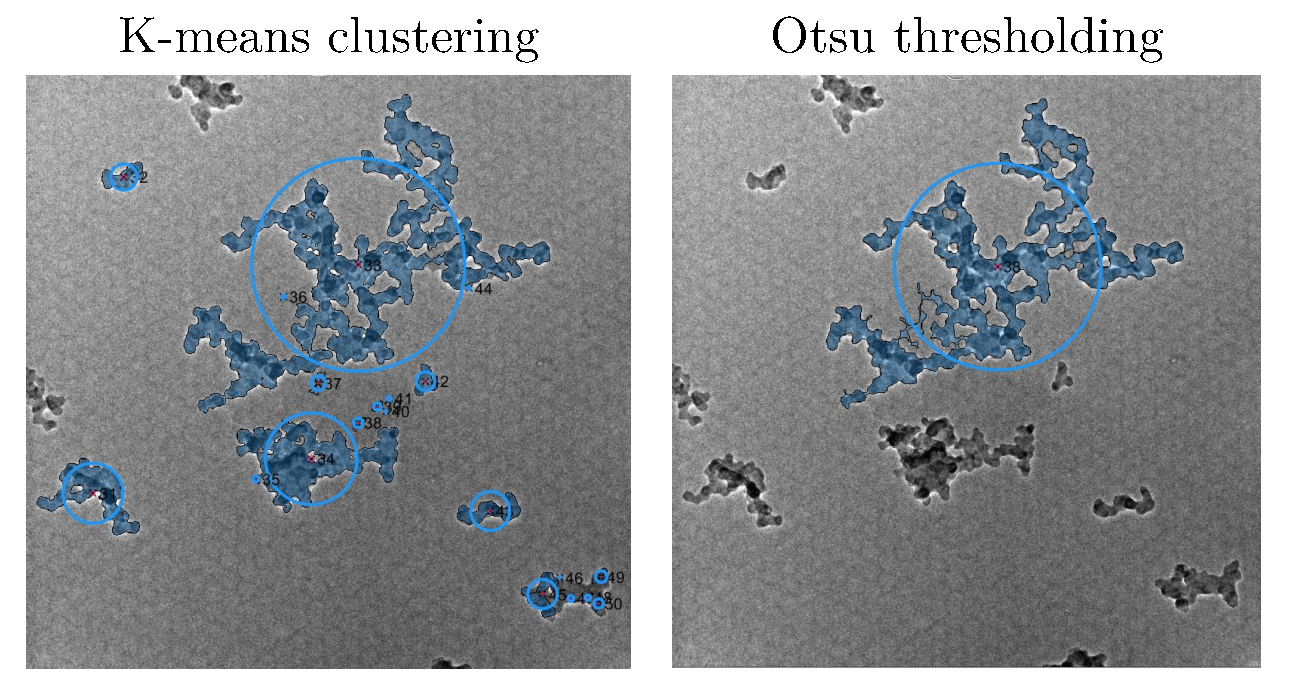
\includegraphics[width=0.6\textwidth]{Figures/Results/Shocktube/Stanford/TEM/aggseg_compare.pdf}
	\caption{Agglomerates in single TEM image segmented by K-means clustering (left pane) and otsu thresholding (right pane)}
	\label{fig:shocktubest_aggseg_compare} 
\end{figure}


\begin{table}
	\caption{The morphological characteristics of agglomerates quantified by atems using KMC and PCM}
	\label{tab:shocktube_TEM_morph}
	\centering
	\begin{tabular}{l l l}
		\hline
		Property & Arithmetic mean & Median \\
		\hline
		$d_m$ [nm] & 97 & 69 \\
		$d_p$ [nm] & 22 & 18 \\
		\hline
	\end{tabular}
\end{table}


Table~\ref{fig:shocktubest_aggseg_compare} reports the arithmetic mean and median of mobility and primary particle diameter detected by atems from TEM images. The computed $d_m$ and $d_p$ will be compared with soot sampled from various sources. Soot morphology is mainly governed by coagulation leading to self-similar structures in which $d_m$ scales with $d_p$ and $n_p$. 
%Following that principle, a power-law derived from DEM simulation in flame conditions~\citep{Kelesidis2017} was introduced in Sec.~\ref{sec:sootmorphology}. Here, we compare the ratio of mobility to primary particle diameter $d_m/d_p$ with $d_m/d_p=n_p^{0.45}$ (Eq.~\ref{eqn:d_m}). 
\citet{olfert2019universal} analyzed soot particles from flares~\citep{kazemimanesh2019size}, inverted burners~\citep{dastanpour2017variation}, compression ignition engines~\citep{graves2015characterization} and other sources to support the external mixing hypothesis and related agglomerate size characterized by $d_m$ to $d_p$ using the following power-law:

\begin{equation}
	d_{p} = d_{p,100} 
	\left(
	\frac{d_m}{100 nm}
	\right)^{D_{\mathrm{TEM}}},
	\label{eqn:usf}
\end{equation}

\noindent where $d_{p,100}$ is the average primary particle diameter for for an agglomerate with $d_m$ = 100 nm, and $D_{\mathrm{TEM}}$ is the exponent. Both quantities were obtained by fitting Eq.~\eqref{eqn:usf} to soot sampled from different sources. Fig~\ref{fig:shocktube_TEM_powerlaws} demonstrates the scatter plot of $d_p$ against $d_m$ compared with power-law curves of Eq.~\eqref{eqn:usf} using two sets of prefactor and exponent values, i) $D_{\mathrm{TEM}}$=0.32, $d_{\mathrm{p,100}}$=20.6 nm, and ii) $D_{\mathrm{TEM}}$=0.39, $d_{\mathrm{p,100}}$=20.2 nm taken from average values reported in summary of fit parameters in Table 1 of \citet{olfert2019universal}. The power-law shows a good agreement with quantities that $d_p$ and $d_m$ computed by \textit{atems} can be good representative of soot agglomerates with minimal agglomerate overlap.

\begin{figure}[H]
	\centering
	\begin{subfigure}[t]{0.32\textwidth}
		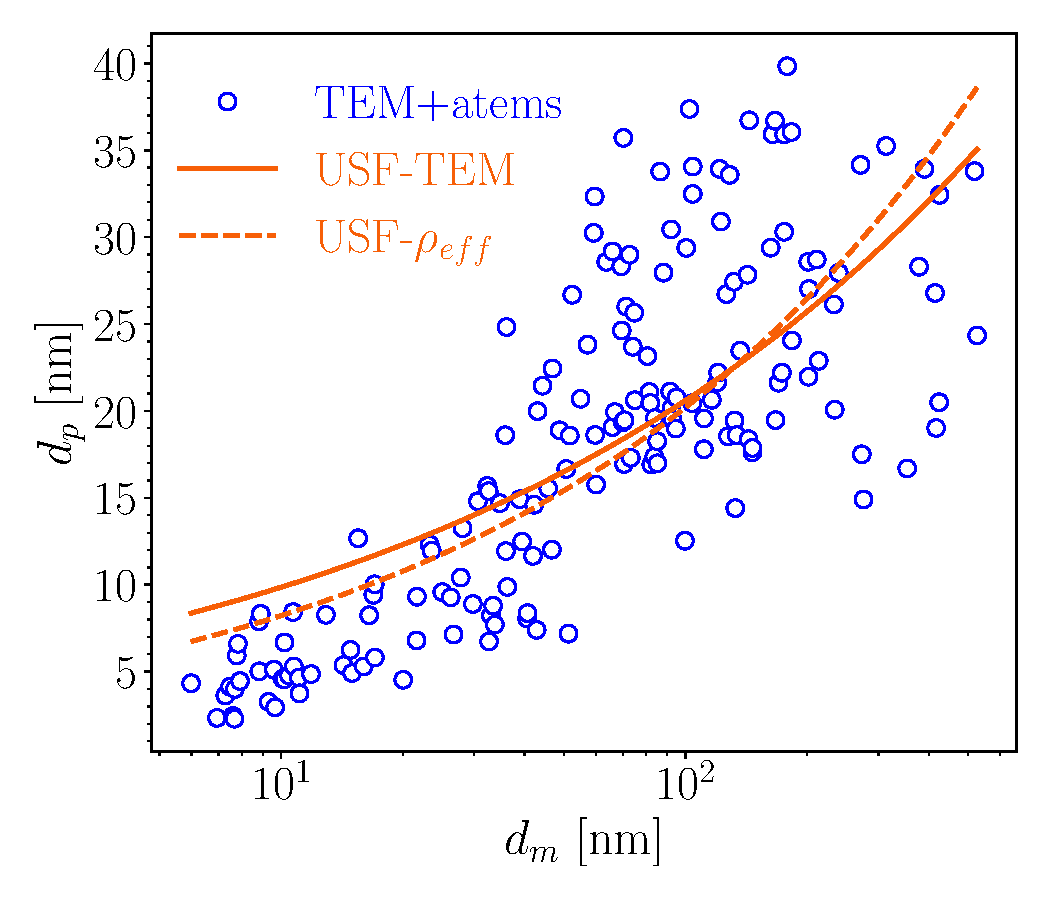
\includegraphics[width=1\textwidth]{Figures/Results/Shocktube/Stanford/TEM/dmdp_scalelaw.pdf}
	\end{subfigure}
	\caption{The $d_m$ as a function of $d_p$ from TEM image obtained by atems~\citep{sipkens2021using} (symbols) compared with the power law in Eq.~\eqref{eqn:usf}} 
	\label{fig:shocktube_TEM_powerlaws} 
\end{figure}

The number of primary particles, $N_{pri}$ was estimated from $f_v$ and $d_p$ assuming spherical primary particles with fixed size during the process. Using minimum, maximum, and mean of $d_p$ from TEM measurements provides a range of expected $N_{pri}$ can be obtained.
\begin{equation}
	N_{pri}=\frac{f_v}{\pi d_p^3/6} 
	\label{eqn:Npriinfered}.
\end{equation}


\subsubsection{Modelling soot yield and morphology}

Fig.~\ref{fig:shocktube_TEM_10ch4_fvNpriIincdp} compares predicted $f_v$ and $d_p$ with data. The horizontal scatter bars denote the uncertainty in the residence time corresponding to the TEM measurement. EBridge Modified and Irreversible Dimerization predicted soot volume fraction in close agreement with measurements, but Reactive Dimerization and Dimer Coalescence overpredict $f_v$ by a factor of 2-3. On the other hand, $d_p$ is significantly underestimated by all PAH growth models. Reactive Dimerization yields the largest $d_p$ nearly 6 nm due to stronger PAH adsorption rate.

\begin{figure}[H]
	\centering
	\begin{subfigure}[t]{0.42\textwidth}
		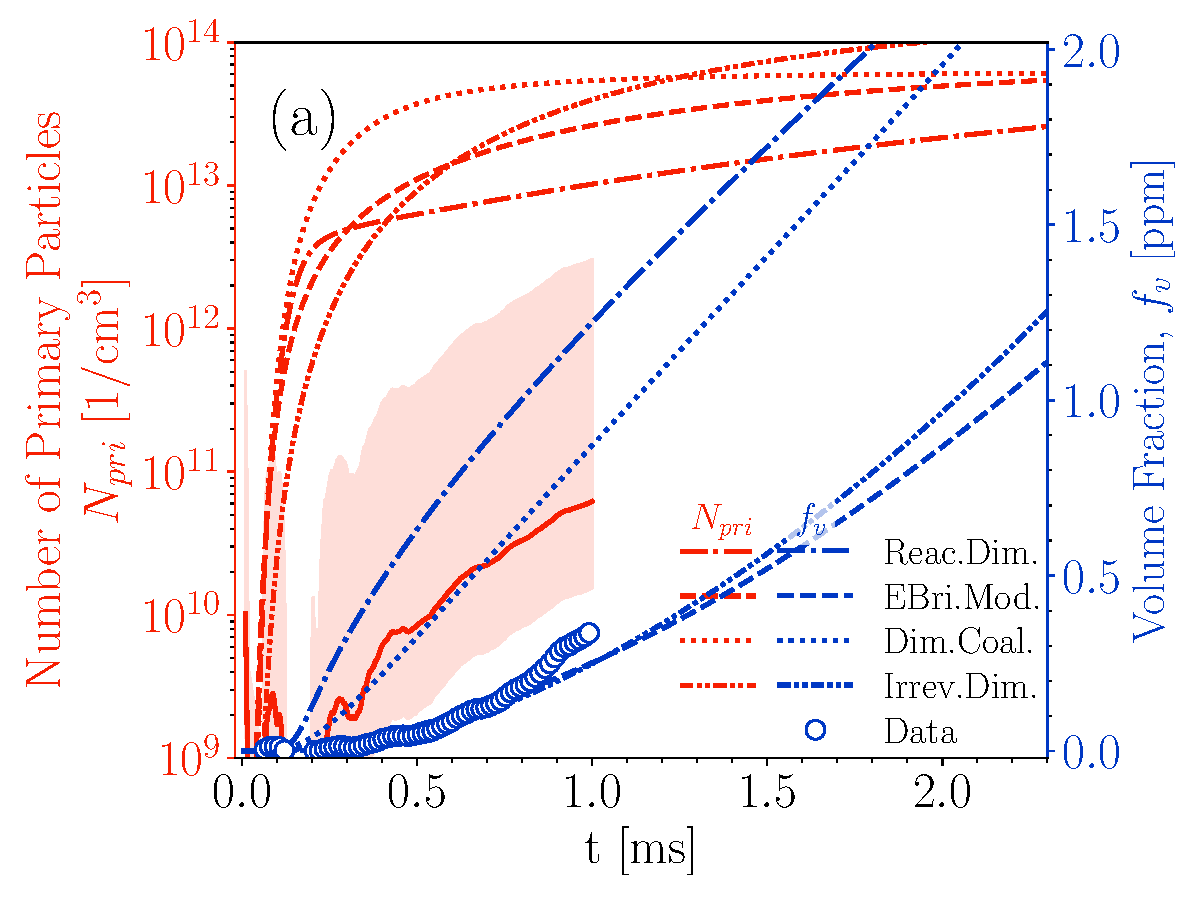
\includegraphics[width=1\textwidth]{Figures/Results/Shocktube/Stanford/TEM/10CH4_TEM_Nprivf.pdf}
	\end{subfigure}
	\begin{subfigure}[t]{0.39\textwidth}
		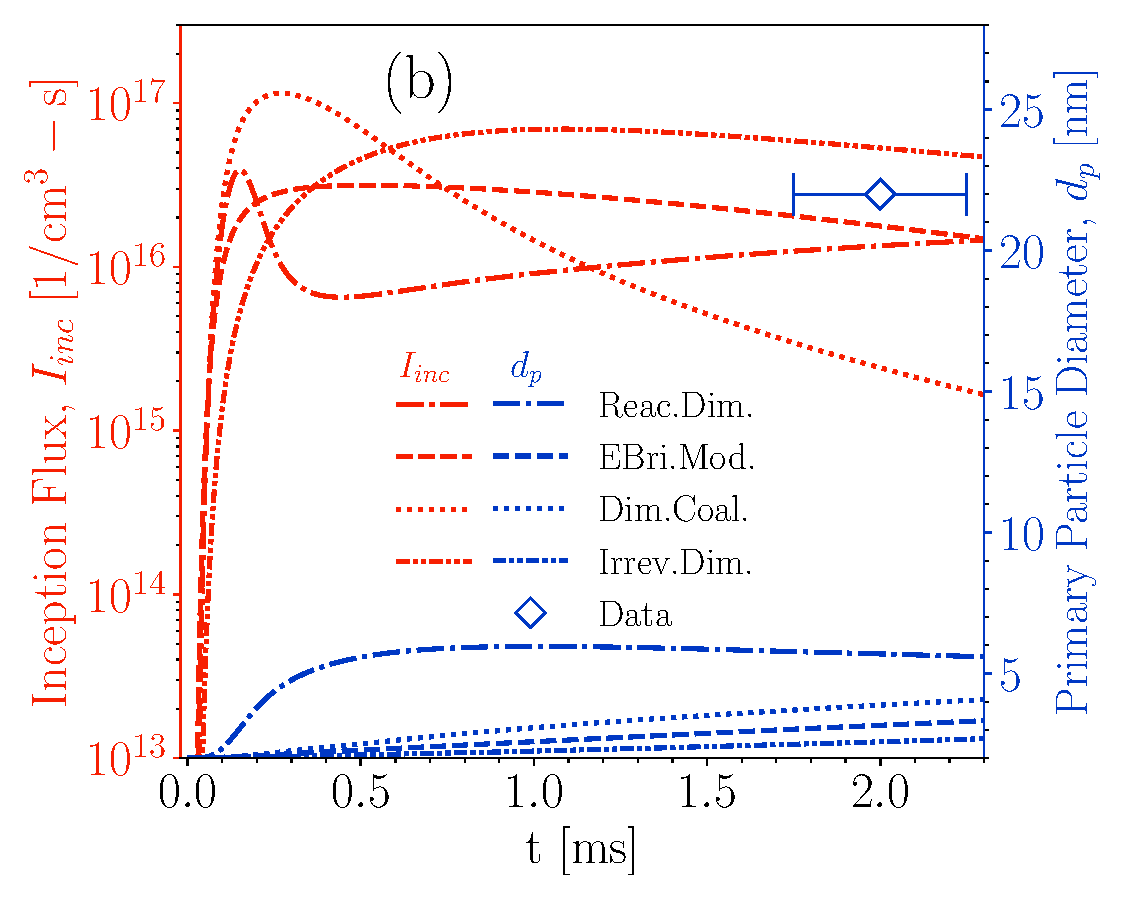
\includegraphics[width=1\textwidth]{Figures/Results/Shocktube/Stanford/TEM/10CH4_TEM_Iincdp.pdf}
	\end{subfigure}
	\caption{The soot volume fraction, $f_v$ and number of primary particles, $N_{pri}$ (left pane), and , the soot inception flux, $I_{inc}$ and the primary particle diameter, $d_p$ predicted by KAUST mechanism, SPBM, and different PAH growth models at T=2230 K, P=4.5 atm that corresponds to shock-tube conditions of TEM measurement}
	\label{fig:shocktube_TEM_10ch4_fvNpriIincdp} 
\end{figure}


The underprediction of $d_p$ by the PAH growth models despite producing enough or even more soot carbon mass compared with the measurement motivated a sensitivity analysis for soot yield and morphology.%, especially because of uncertainties in inception and surface growth pathways and reaction rates associated with the PAH growth models integrated in omnisoot.
It should be noted that the sensitivity analysis is only focused on soot model to identify the sub-model(s) with the dominant effect on yield and morphology, and it does not include reactions in the gas phase.

First, the effect of HACA rate on soot yield and morphology is examined for the data point with T=2230 K and P=4.5 atm. To this purpose, the surface reactivity, $\alpha$, in HACA formulation is modified by introducing a damping factor, $\zeta$ in Eq.~\eqref{eqn:hacaRate} as:

\begin{equation}
	\alpha^i = \tanh 
	\left(
	\frac{12.56 - 0.00563\cdot \zeta T}
	{\mbox{log}_{10}
		\left( \frac{\rho_{soot}\cdot Av}{W_{carbon}} \frac{\pi}{6}{d^i_p}^3 \right) } -1.38+0.00068\cdot \zeta T
	\right)
	\label{eqn:alpha_modified}.
\end{equation}

Note that, there are many adjustable parameters in HACA scheme such as rate constants. We picked $\zeta$ to modify $\alpha$ for a number of reasons: First, $\alpha$ was initially introduced as a tuning parameter as a function of local temperature and primary particle diameter to control surface growth rate, and it has been usually adjusted specifically for each flame~\citep{castaldi1996pah, xu1997soot} to match the predicted volume fraction with the measurements. Second, the global empirical relation of \citet{appel2000kinetic} (used in omnisoot to quantify $\alpha$) developed by fitting parameters of $\alpha$ to minimize the prediction error of volume fraction for various premixed flames, but shock tubes generally have larger temperature ranges compared with premixed flames, which could excessively reduce surface reactivity and HACA growth rates. Finally, larger volume fractions (in the order of few ppm) were underpredicted by the global $\alpha$ relation (Fig.~9 of \citep{appel2000kinetic}). So, the low values of $\alpha$ in the shock tube at T=2230 K corresponding to process conditions of TEM measurements can contribute to underprediction of surface growth rates and $d_p$. We introduce $\zeta$ to reduce the damping effect of temperature on surface reactivity that promote HACA growth rates resulting in larger primary particle diameters, and possibly lessen the discrepancy between predicted and measured $d_p$. Fig.~\ref{fig:shocktube_alpha_HACA} demonstrates the variation of $\alpha$ with temperature for $\zeta$=0.6, 0.8, 1 and primary particle diameter 2 and 6 nm. $\alpha$ decreases with temperature, and it is inversely proportional to $\zeta$. 

\begin{figure}[H]
	\centering
	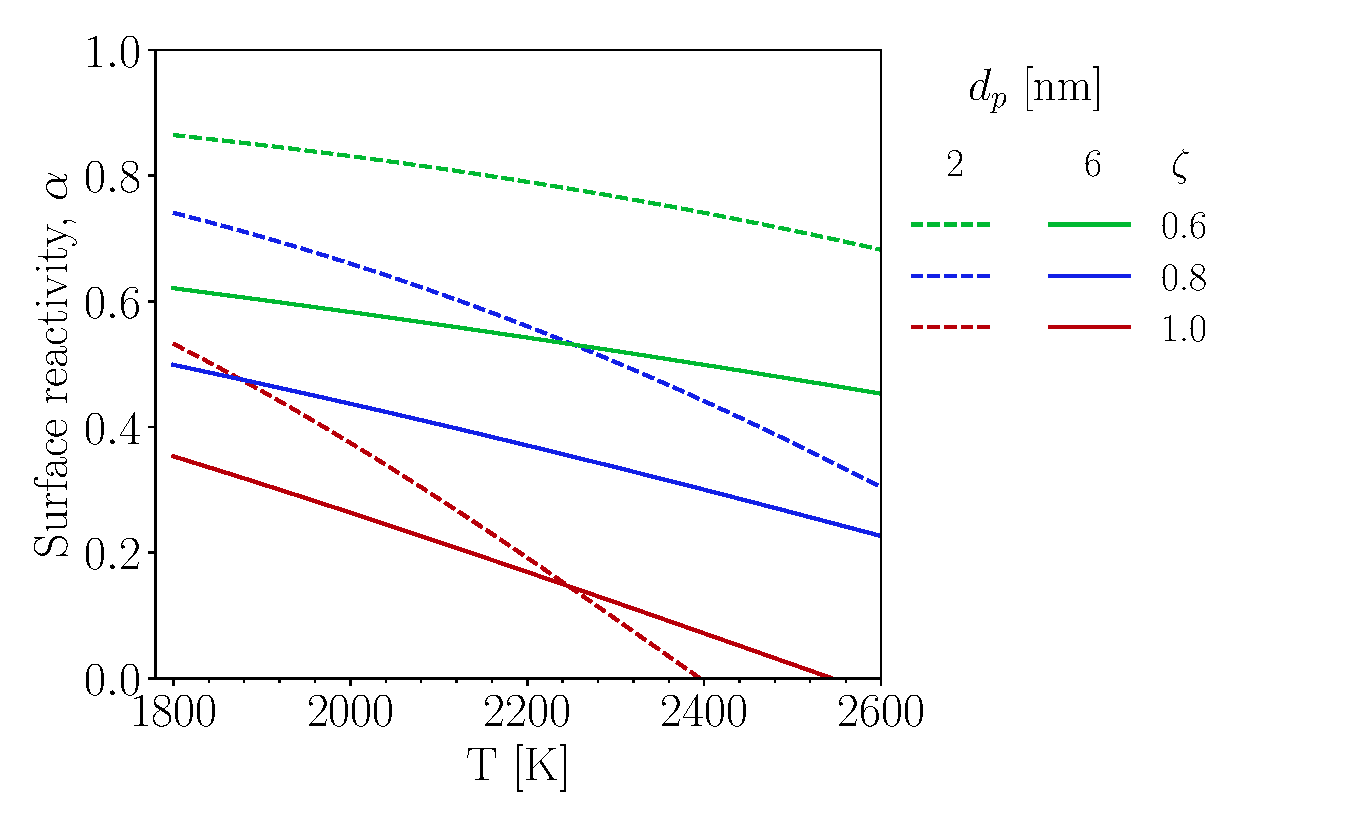
\includegraphics[width=0.5\textwidth]{Figures/Results/Shocktube/HACA/alpha.pdf}
	\caption{The variation of surface reactivity, $\alpha$, as a function of temperature for different values of $\zeta$ and primary particle size of 2 nm (dashed lines) and 6 nm (solid lines)}
	\label{fig:shocktube_alpha_HACA} 
\end{figure}

A series of simulations was performed to study the damping effect of temperature on soot mass and morphology by varying  $\zeta$ from 1 to 0.8 and 0.6. Note that, $\zeta$ of 1 represent the original $\alpha$ formulation. The reaction mechanism and particle dynamic model were set to KAUST and SPBM, respectively.
Fig.~\ref{fig:shocktube_vf_zetseffect} depicts the volume fraction variation for each PAH growth model using different $\zeta$ values. As expected, lowering $\zeta$ increases the soot volume fraction with a maximum of 29\% at t=2 ms for Dimer Coalescence. However, as shown in Fig.~\ref{fig:shocktube_dp_zetseffect} $\zeta$ has negligible effect on $d_p$ with all PAH growth models. As a result, HACA growth rate cannot account for the observed gap between measure and predicted primary particle within 2 ms of the simulation of shock tube.

\begin{figure}[H]
	\centering
	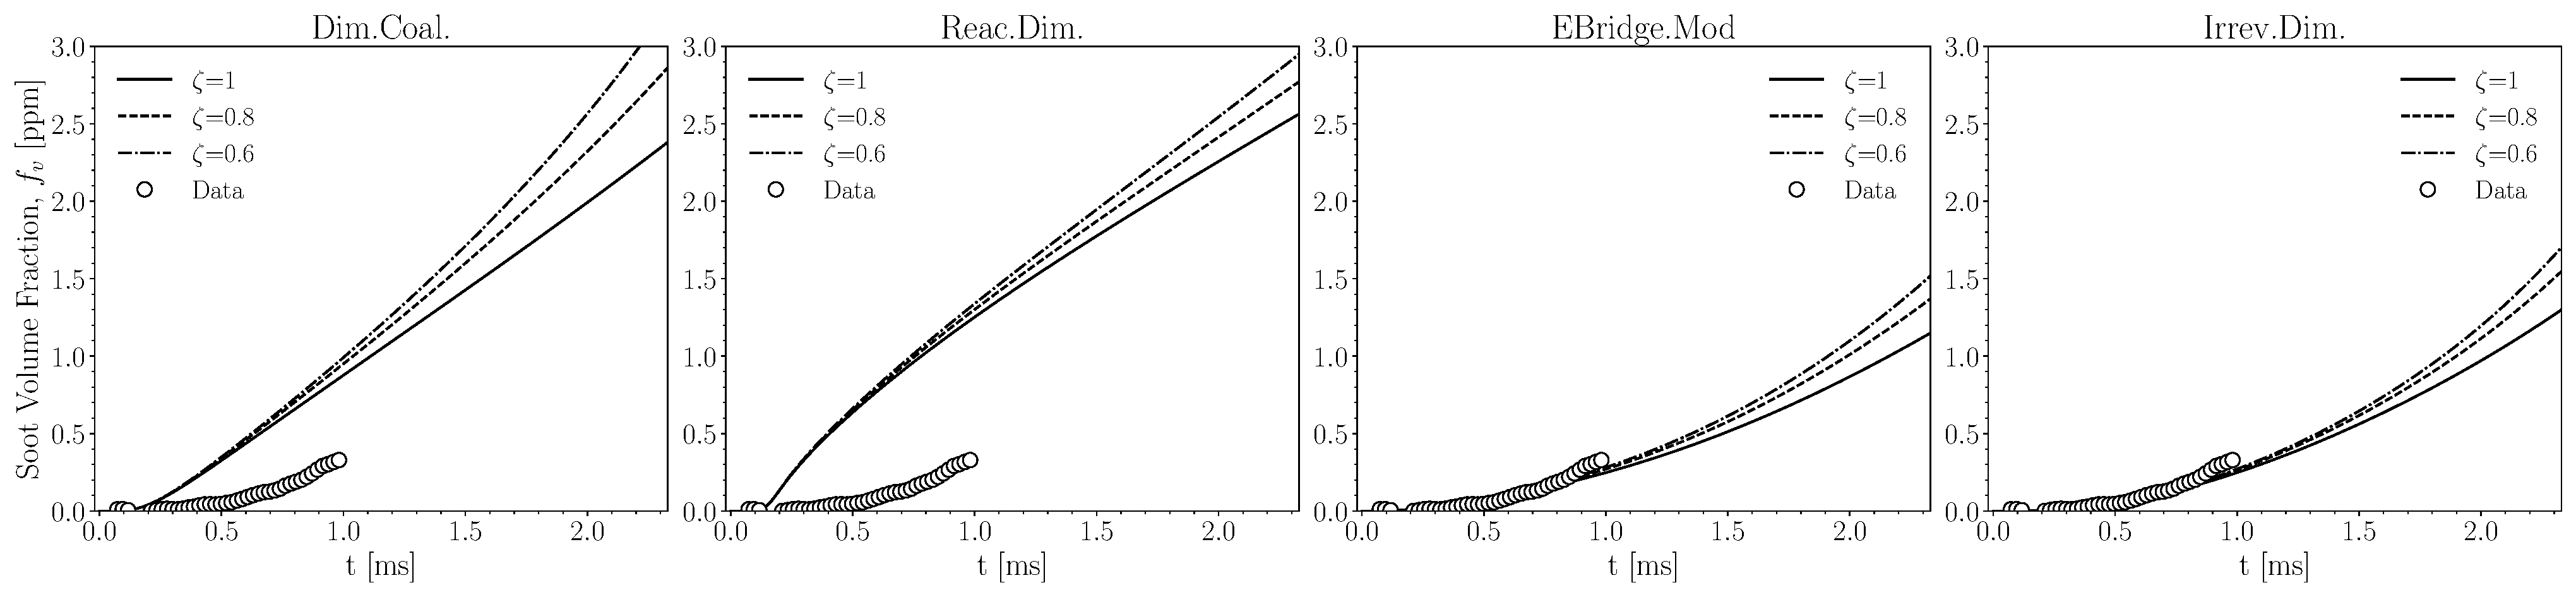
\includegraphics[width=1\textwidth]{Figures/Results/Shocktube/Stanford/TEM/10CH4_TEM_vf_HACAsens.pdf}
	\caption{The effect of reducing $\zeta$ leading to larger HACA rates on soot volume fraction, $f_v$ using KAUST, SPBM and different PAH growth model}
	\label{fig:shocktube_vf_zetseffect} 
\end{figure}


\begin{figure}[H]
	\centering
	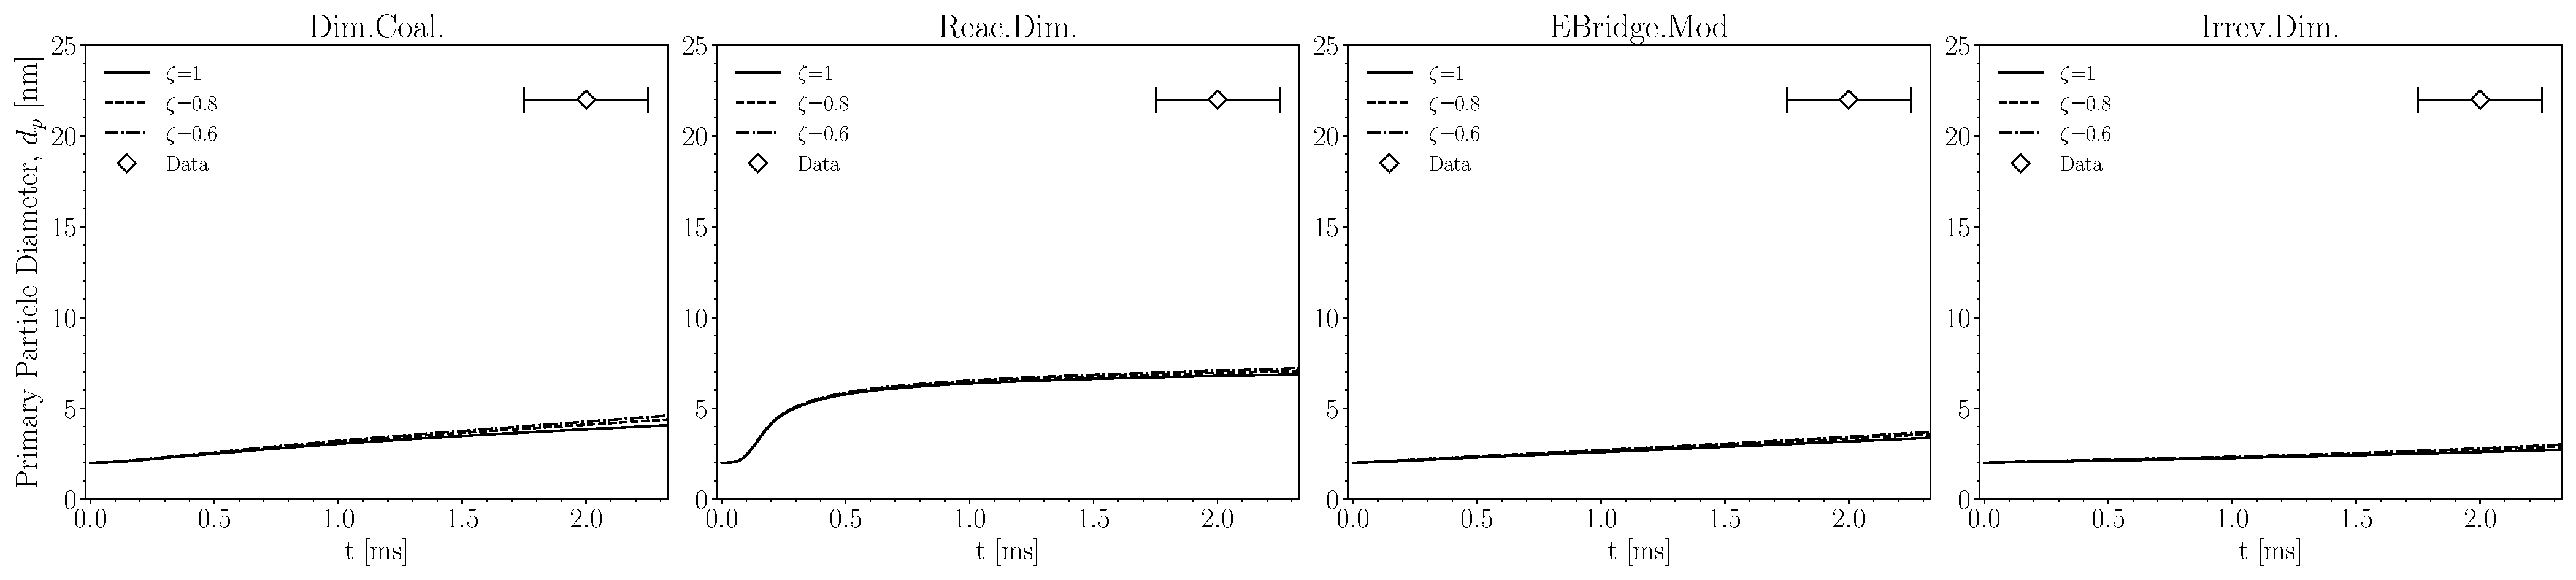
\includegraphics[width=1\textwidth]{Figures/Results/Shocktube/Stanford/TEM/10CH4_TEM_dp_HACAsens.pdf}
	\caption{The effect of reducing $\zeta$ leading to larger HACA rates on primary particle diameter, $d_p$ using KAUST and MPBM and different PAH growth model}
	\label{fig:shocktube_dp_zetseffect} 
\end{figure}

There is evidence supporting the coalescence (or sintering) of soot particles at initial stages of formation. The TEM images collected thermophoretically~\citep{zhao2007comparative} near the inception zone of a burner-stabilized laminar premixed ethylene–oxygen–argon flame ($\phi$ = 2.5) showed particles with apparent sizes larger than those measured by Scanning Mobility Particle Sizer (SMPS)~\citep{oktem2005chemical} suggesting that the particles flatten on the TEM grid upon impact. In other words, incipient and nascent soot particles may have a liquid-like state that quickly transforms to a fully solid particles due to soot aging and maturity \citep{kholghy2016core}. At intial stages, these particle can coalesce (merge) upon collision forming larger primary particles. There are a few experimental studies on soot coalescence. \citet{ono2017experimental} reheated size-selected particles with a differential mobility analyzer formed during pyrolysis of ethylene and benzene in a secondary reactor and observed the morphological changes by comparing the TEM images. \citet{matsukawa2023experimental} proposed a relation based on solid-state sintering mechanism of metalic nano-particles to describe characteristic sintering time of soot as:

\begin{equation}
	\tau^i_c = A (d^i_p)^4 \cdot T \cdot exp(\frac{E_a}{RT}),
	\label{eqn:coalcharactime}
\end{equation}

\noindent where $A=3.01×10^{22} \mathrm{[s/m^4-K]}$ and $E_a = 1.40×10^5 \mathrm{[J/mol]}$ are the prefactor, and activation energy, respectively, that are determined by curve-fitting to the change in primary particle diameter of soot after reheating in a flow reactor. Coalescence does not affect the agglomerate mass, but rather decreases the surface area of an agglomerate by merging primary particles. Coalescence is described in omnisoot by adding another partial source term to Eq.~\ref{eqn:S_Nprisect} as:

\begin{equation}
	\left(S_{N_{pri}}\right)_{coal} = 
	- \frac{3}{\tau^i_c}
	\left(
		n^i_p - \left(n^i_p\right)^{2/3}
	\right) N^i_{agg}
	\label{eqn:S_Npricoal}
\end{equation}

Fig.~\ref{fig:shocktube_vf_coaleffect} depicts the decrease in $f_v$ by considering coalescence because of reduction in the surface area of agglomerates hence the number of active sites for HACA growth. As shown in Fig.~\ref{fig:shocktube_dp_coaleffect}, coalescence increases $d_p$ with a maximum of 64\% for Dimer Coalescence, but it cannot account for the significant underprediction of primary particle diameter by the model.

\begin{figure}[H]
	\centering
	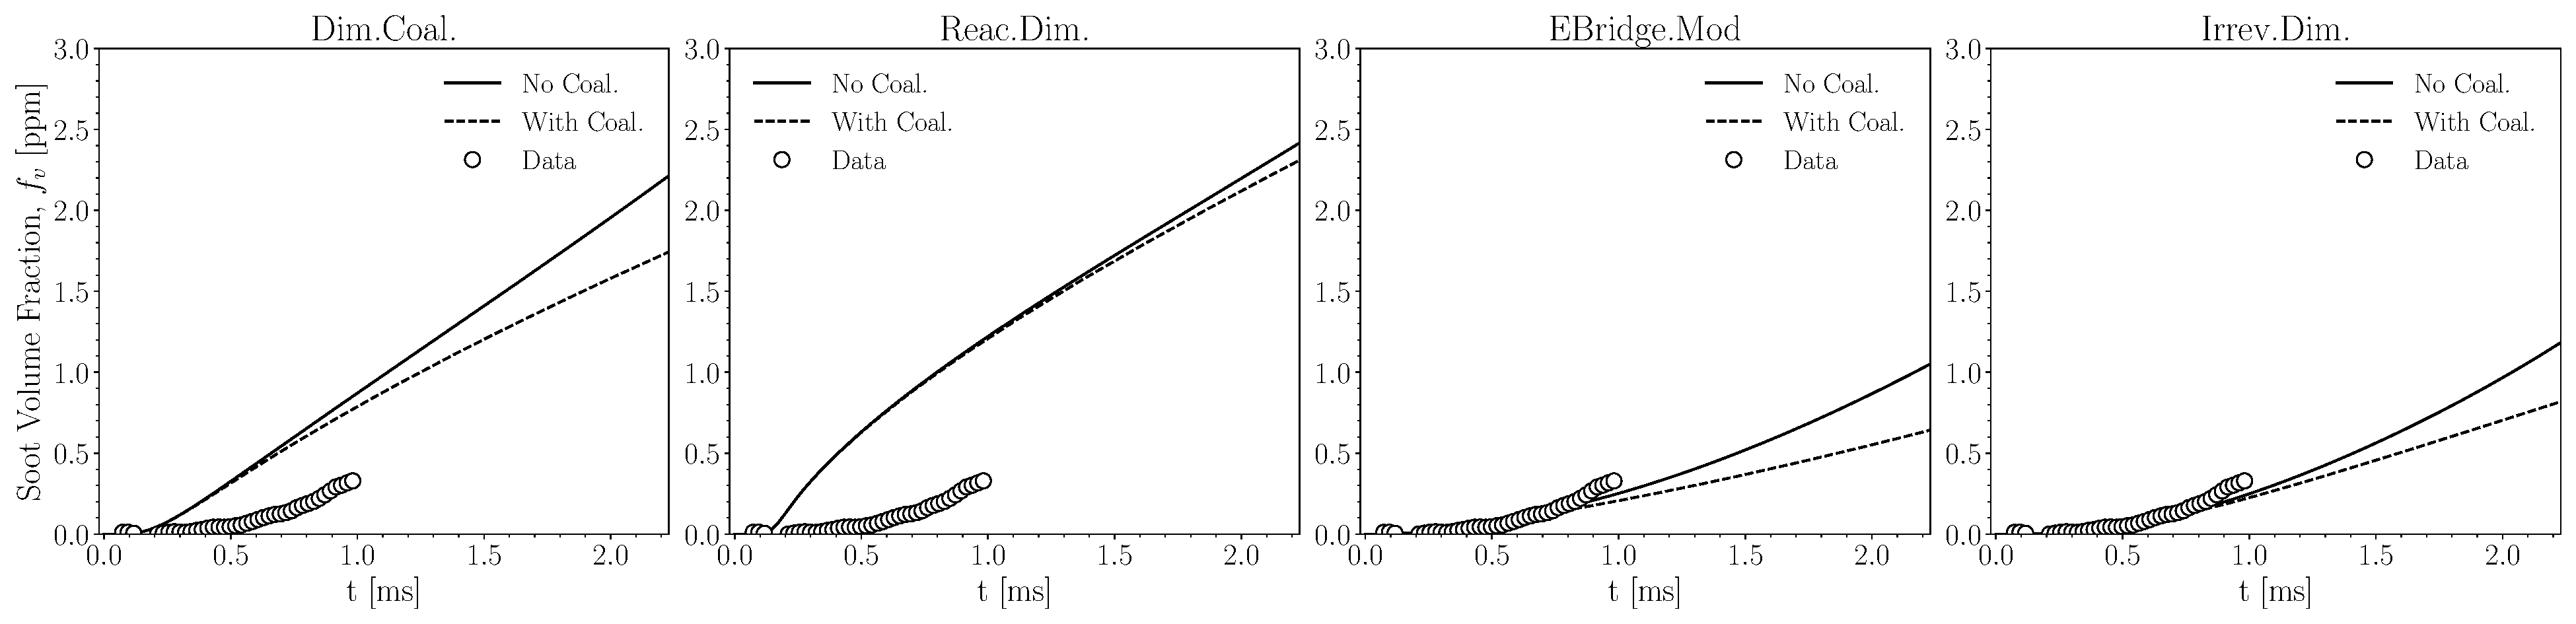
\includegraphics[width=1\textwidth]{Figures/Results/Shocktube/Stanford/TEM/10CH4_TEM_vf_coalesens.pdf}
	\caption{The effect of coalescence onsoot volume fraction, $f_v$ using KAUST, SPBM and different PAH growth model}
	\label{fig:shocktube_vf_coaleffect} 
\end{figure}


\begin{figure}[H]
	\centering
	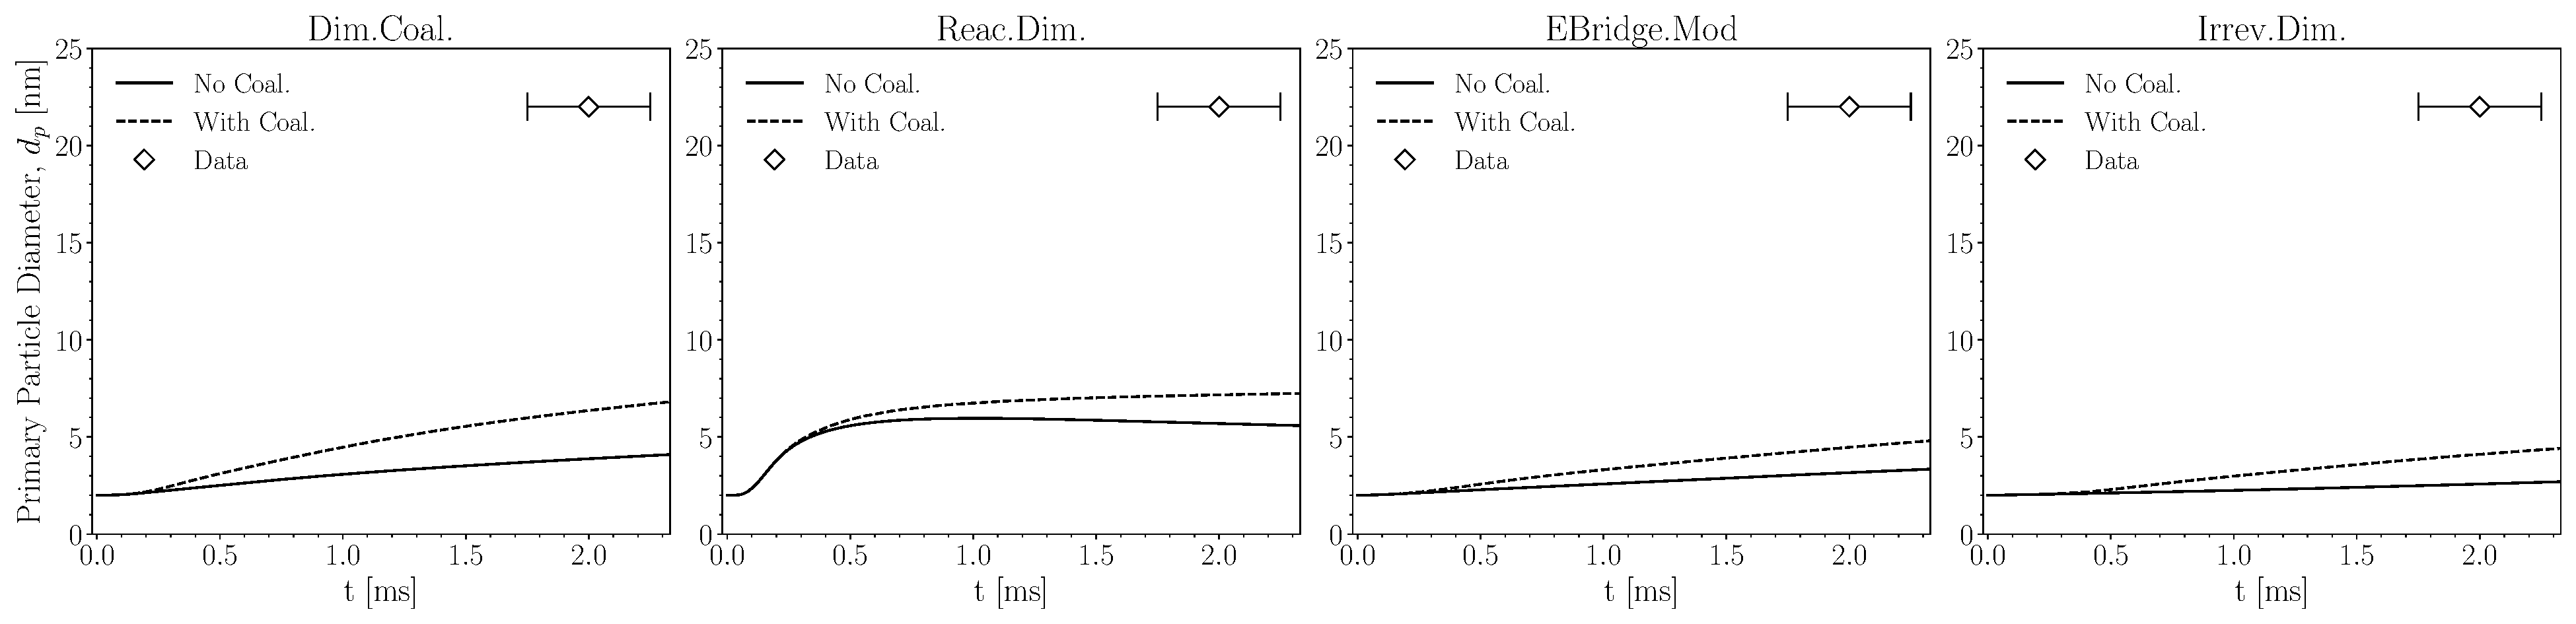
\includegraphics[width=1\textwidth]{Figures/Results/Shocktube/Stanford/TEM/10CH4_TEM_dp_coalesens.pdf}
	\caption{The effect of coalescence on primary particle diameter, $d_p$ using KAUST and SPBM and different PAH growth model}
	\label{fig:shocktube_dp_coaleffect} 
\end{figure}

The next step is examining the effect on inception and PAH adsorption on predicted soot volume fraction and primary particle diameter. This is achieved by introducing two prefactors, $\delta$ and $\eta$ to adjust inception flux and PAH adsorption rate, respectively. Nine different simulation cases are designed by assigning 1, 0.01, 0.001 to $\delta$ and 1, 10, 100 to $\eta$ where the case with $\delta, \eta=1$ corresponds to the default PAH growth parameters. Fig.~\ref{fig:shocktube_vf_incepPAHRD} and \ref{fig:shocktube_dp_incepPAHRD} shows modifying $\delta$ and $\eta$ values in Reactive Dimerization model can significantly change the $f_v$ and $d_p$. Modified primary particle diameter values increased large enough to cover the gap between TEM measurements and simulations. By introducing the same prefactors in the rest of PAH growth model, we noticed that $d_p$ exhibits a similar sensitivity with respect to $\delta$ and $\eta$ values. Therefore, the inception flux and increasing the PAH adsorption rate are the major factors that determine primary particle size and soot yield in shock-tube simulations.


\begin{figure}[H]
	\centering
	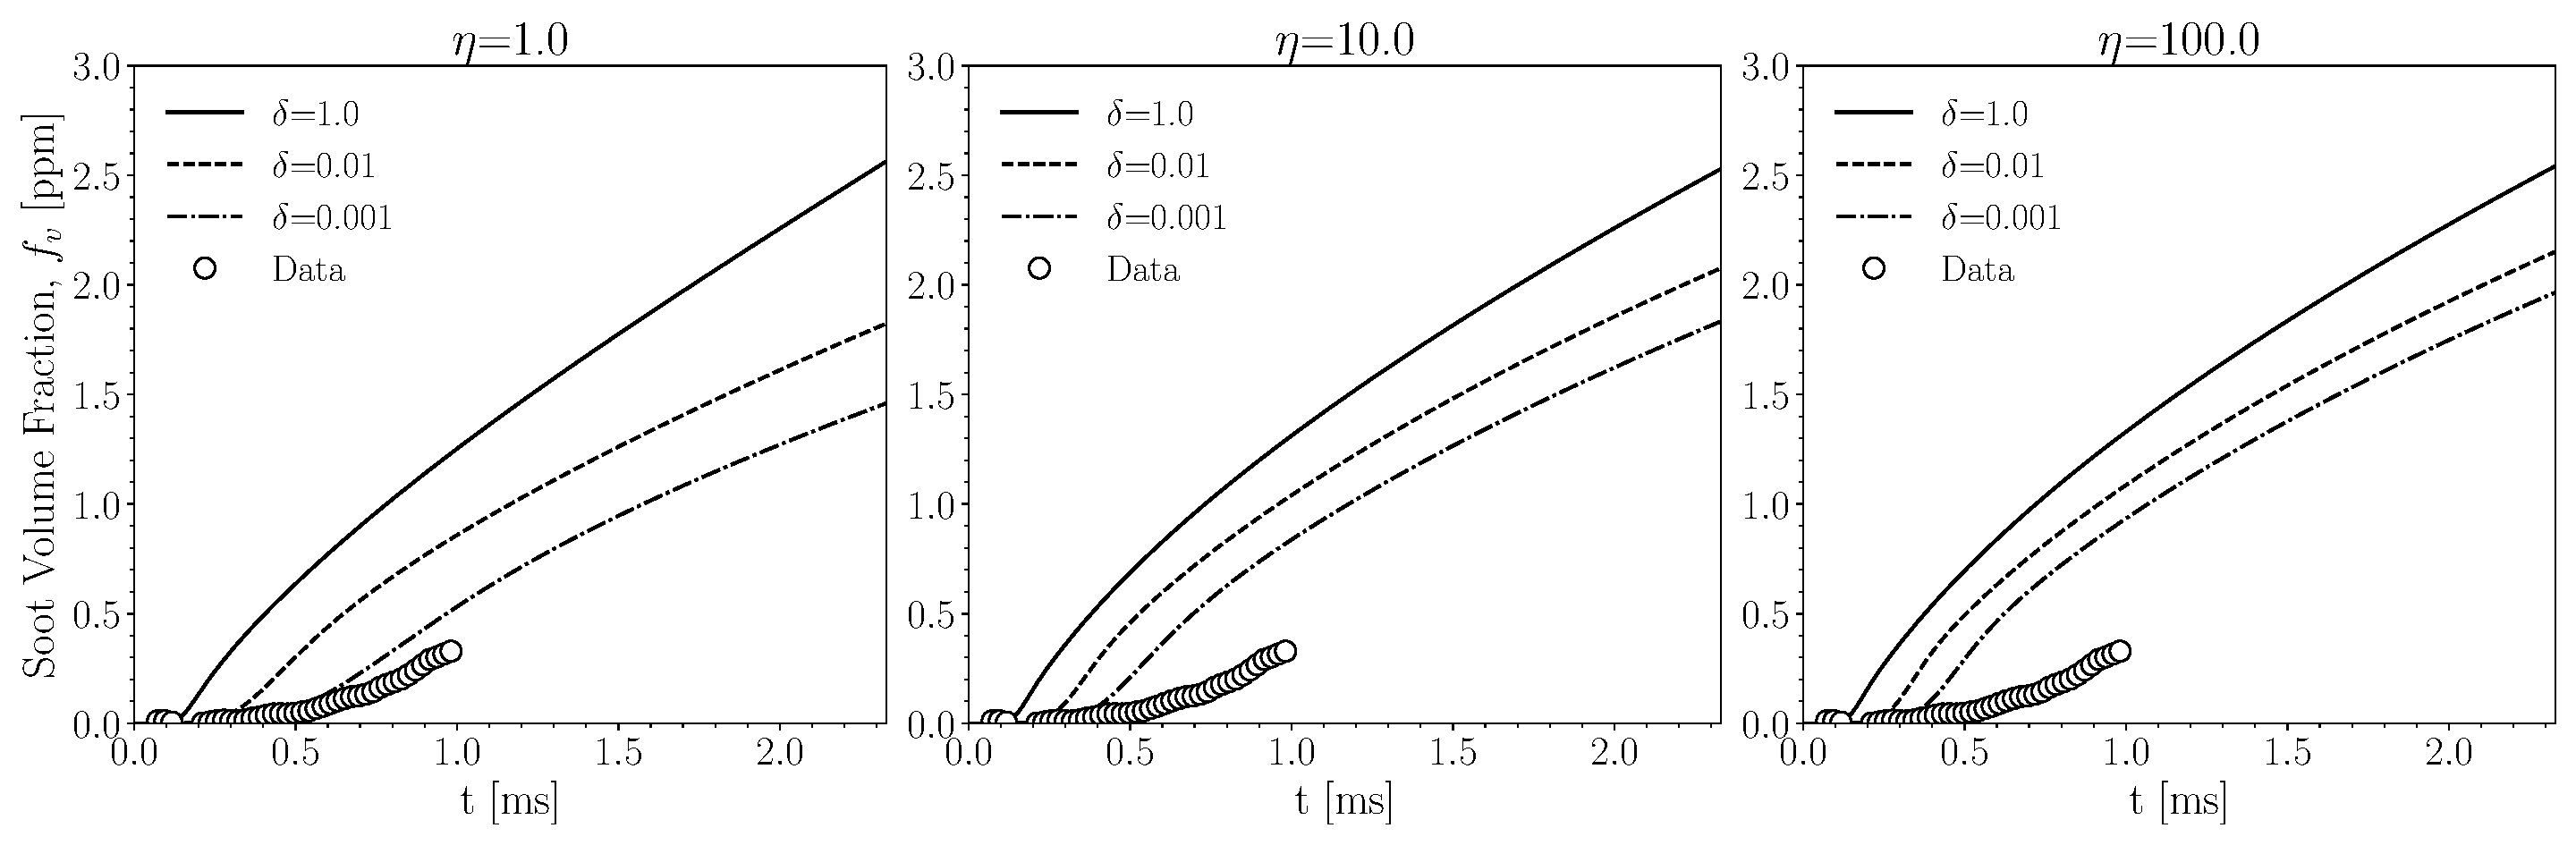
\includegraphics[width=1\textwidth]{Figures/Results/Shocktube/Stanford/TEM/10CH4_TEM_vf_incepPAHsens.pdf}
	\caption{The effect of inception flux and PAH adsorption rate on soot volume fraction, $f_v$, using KAUST, Reactive Dimerization and SPBM}
	\label{fig:shocktube_vf_incepPAHRD} 
\end{figure}


\begin{figure}[H]
	\centering
	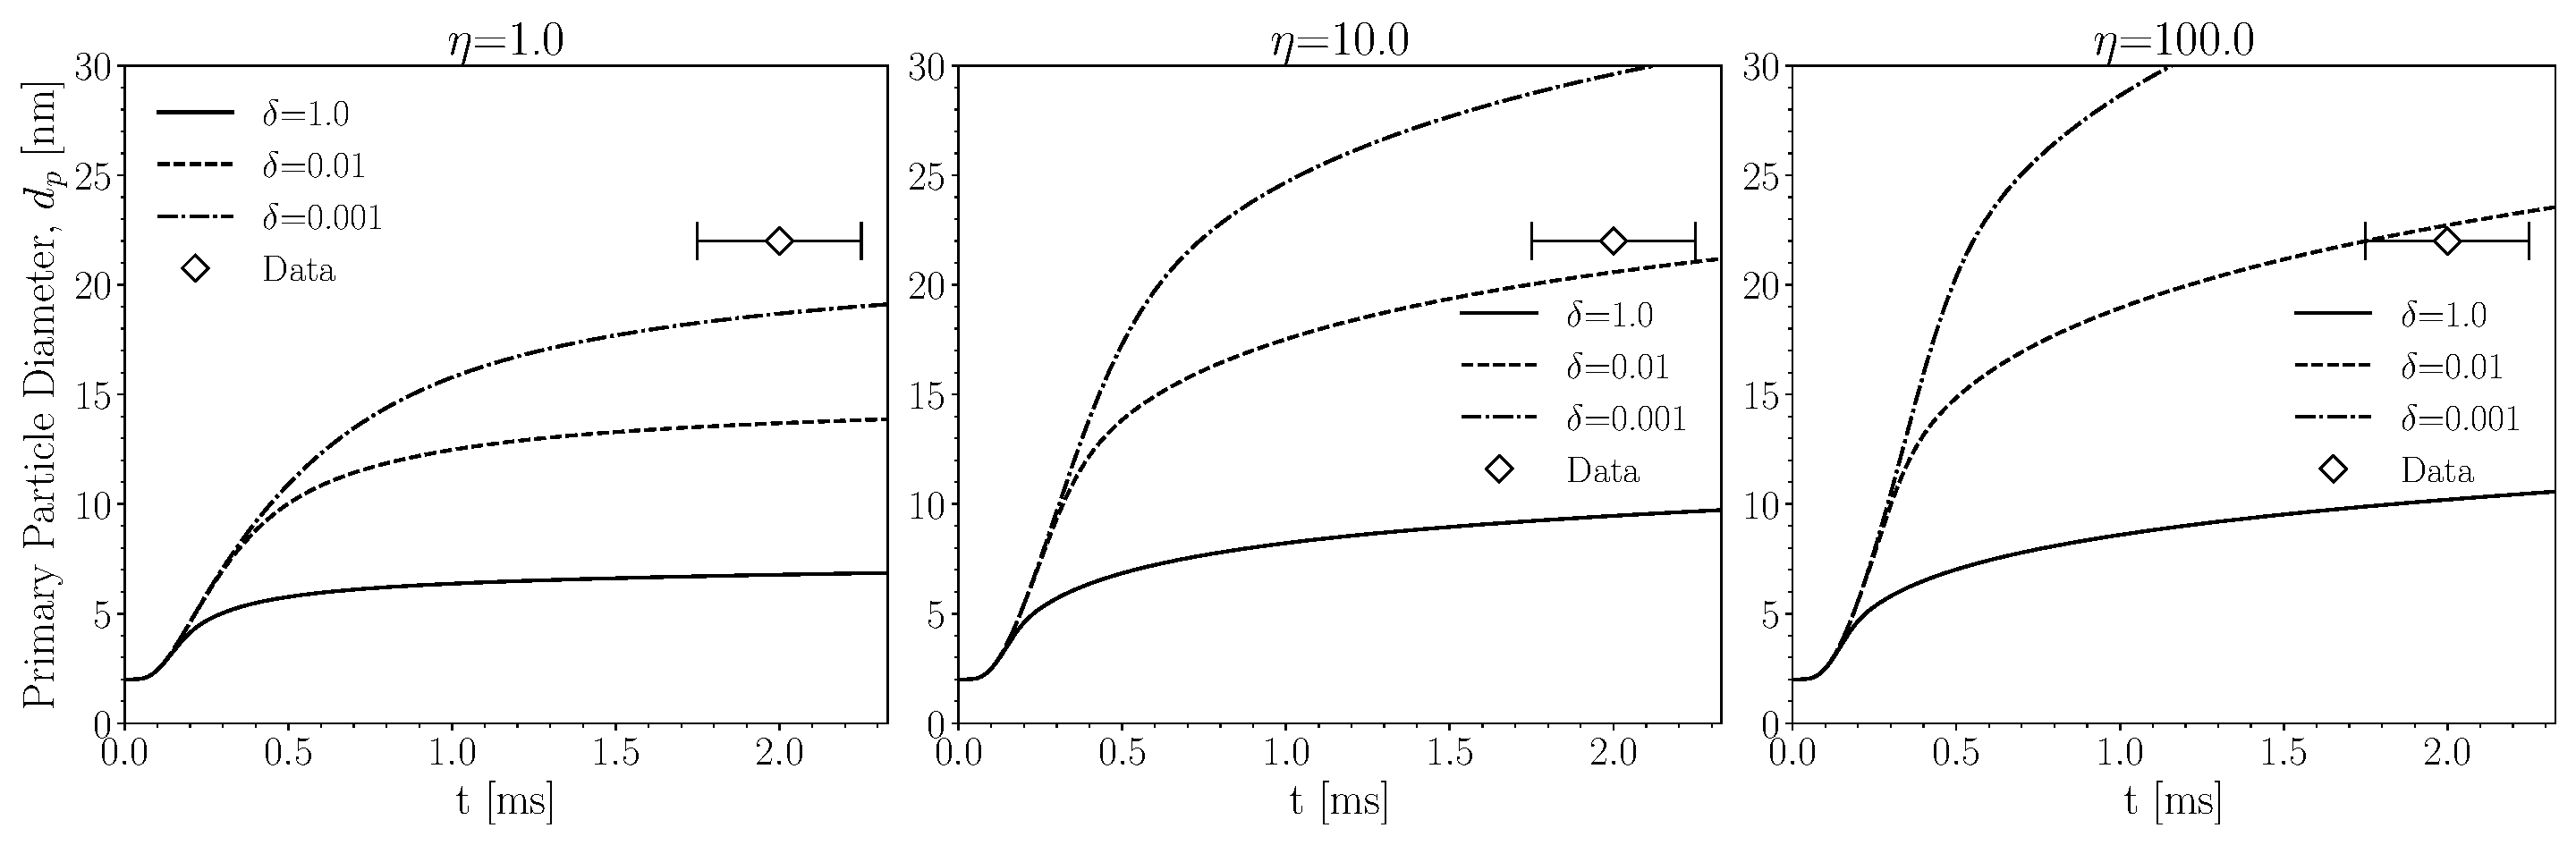
\includegraphics[width=1\textwidth]{Figures/Results/Shocktube/Stanford/TEM/10CH4_TEM_dp_incepPAHsens.pdf}
	\caption{The effect of inception flux and PAH adsorption rate on primary particle diameter, $d_p$ using KAUST, Reactive Dimerization and SPBM}
	\label{fig:shocktube_dp_incepPAHRD} 
\end{figure}

Now that the importance of inception and PAH adsorption is demonstrated, a systematic analysis will be conducted for each PAH growth model by altering $\delta$ and $\eta$ to determine the rate constants that minimize the prediction error of both $f_v$ and $d_p$. The weighted average of mean square error of $f_v$ and  $d_p$ was used to calculate the total error. We employ a two-step grid search for all PAH growth models. In the first step, both $\delta$ and $\eta$ are divided and multiplied by a series factors ranging 1-$10^4$, respectively, leading to 81 simulations in total. The simulation case with the lowest error is used as the starting point for the second grid search by perturbing $\delta$ and $\eta$ between -50\% and +50\%, leading to 45 simulations. It is important to note that the purpose of optimization is not necessarily finding the global minimum of cost function (the combined error of $d_p$ and $f_v$), but rather to show that it is possible to predict both $f_v$ and $d_p$ in good agreement with data by adjusting the inception flux and PAH adsorption rate ensuring that the rate constants stay within their physical limit. The agreement between data and predictions using optimized PAH growth models shown in Fig.~\ref{fig:shocktube_TEM_10ch4_fvNpriIincdp_opt} confirms the above-mentioned conclusion. Interestingly, the predicted $N_{pir}$ by all PAH growth models reach a plateau of $10^{11} \: [1/cm^3]$ and fall in the range inferred from extinction and TEM measurements. The inception flux, $I_{inc}$ of PAH growth models shows similar behavior spanning over the range of $\approx3\times10^{12} \: [1/cm^3-s]$ to $\approx3\times10^{14} \: [1/cm^3-s]$. But, they also have noticeable differences. While Dimer Coalescence starts with a quick rise in inception flux followed by a decrease toward the end of test time, Reactive Dimerization predicts a more uniform inception over the simulated time. 


\begin{figure}[H]
	\centering
	\begin{subfigure}[t]{0.42\textwidth}
		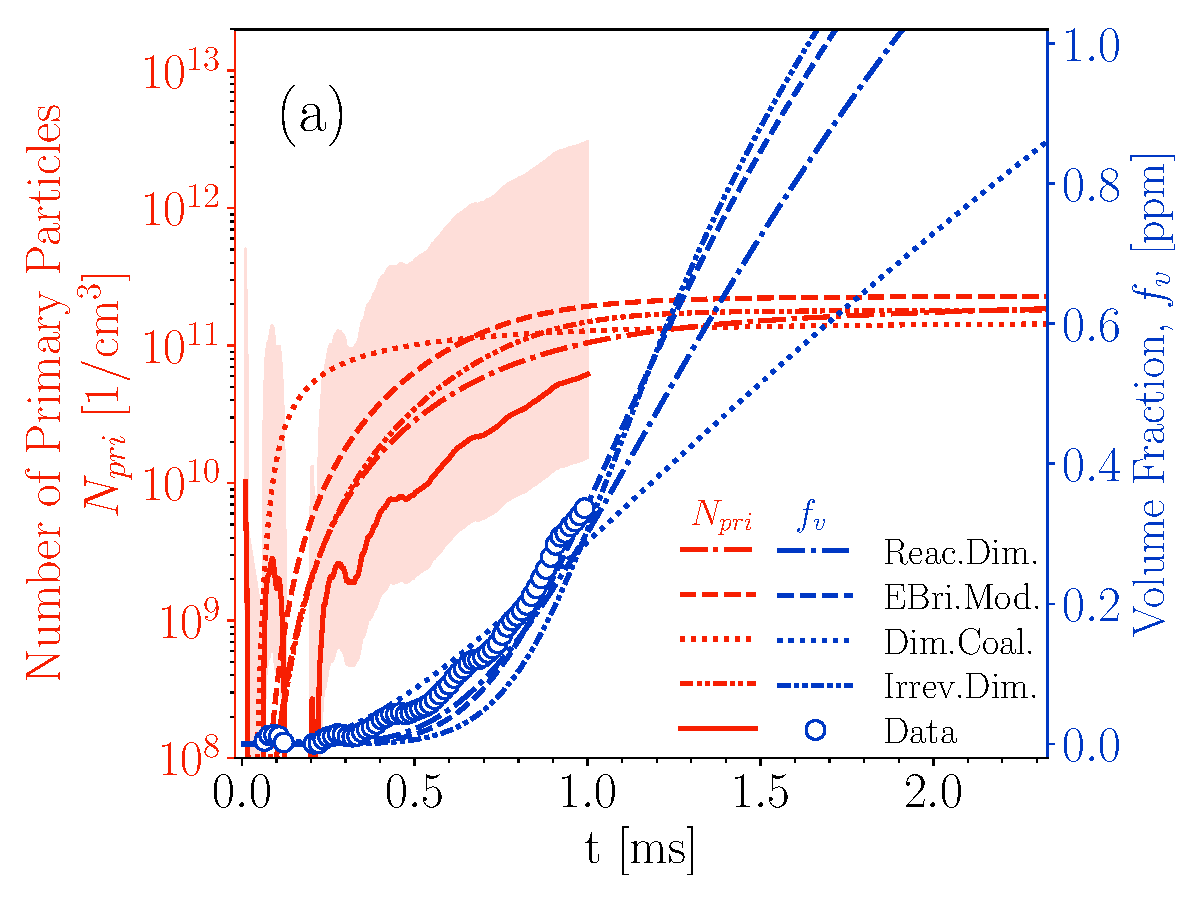
\includegraphics[width=1\textwidth]{Figures/Results/Shocktube/Stanford/TEM/10CH4_TEM_Nprivf_opt.pdf}
	\end{subfigure}
	\begin{subfigure}[t]{0.39\textwidth}
		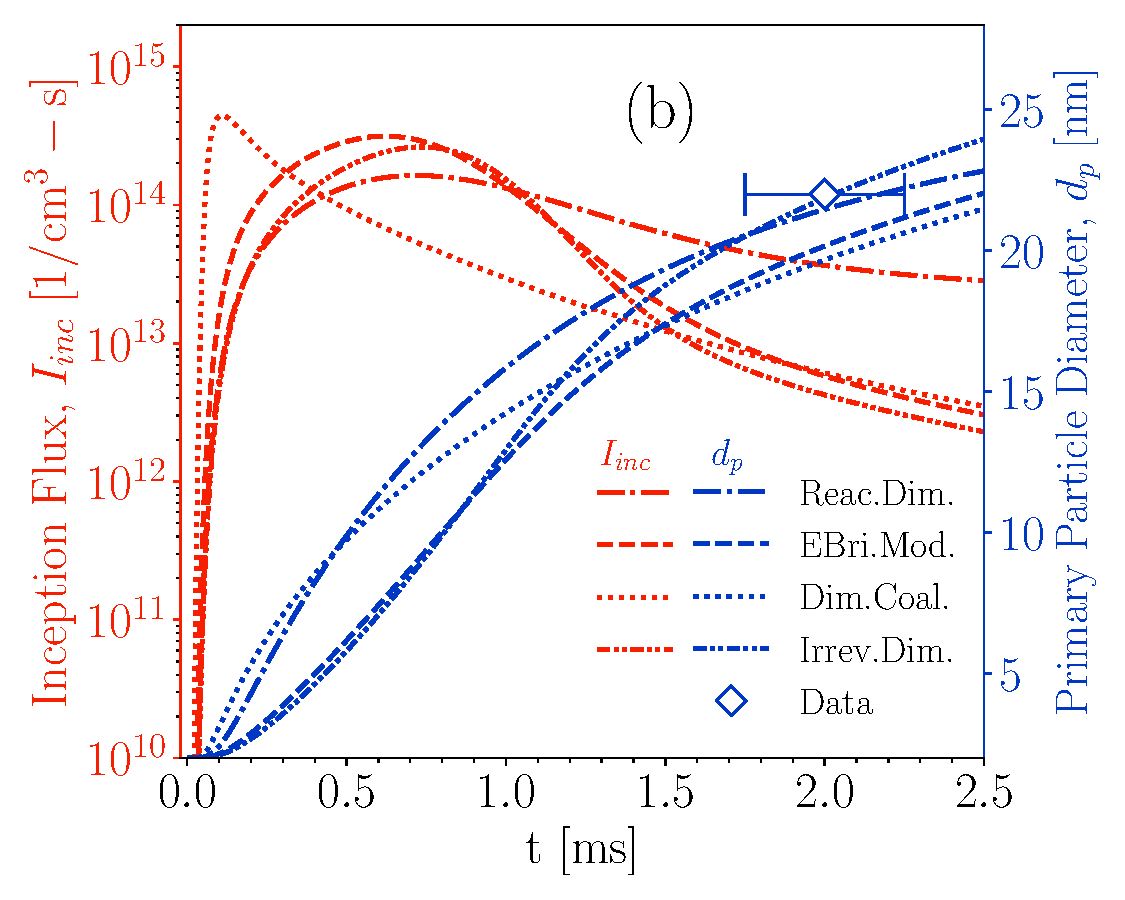
\includegraphics[width=1\textwidth]{Figures/Results/Shocktube/Stanford/TEM/10CH4_TEM_Iincdp_opt.pdf}
	\end{subfigure}
	\caption{The soot volume fraction, $f_v$ and number of primary particles, $N_{pri}$ (left pane), the soot inception flux, $I_{inc}$ and the primary particle diameter, $d_p$ predicted by KAUST mechanism, SPBM, and different PAH growth models with optimized rate at T=2230 K, P=4.5 atm that corresponds to shock-tube conditions of TEM measurement}
	\label{fig:shocktube_TEM_10ch4_fvNpriIincdp_opt} 
\end{figure}

The PAH growth models with optimized rates were applied to the whole temperature and pressure ranges (see Fig.~\ref{fig:shocktubest_10ch4_vf_incepopt_all} and \ref{fig:shocktubest_10ch4_dp_incepopt_all}). As shown in Fig.~\ref{fig:shocktube_10_CH4_vf_incepopt}, the measured $f_v$ demonstrates a relatively strong sensitivity to temperature best captured by EBridge Formation. This model start with a temperature-dependent dehydrogenation step, but other model are initialed with PAH collision that weakly depends on temperature. On the other hand, Dimer Coalescence is least sensitive to temperature. While it slightly underestimates $f_v$ at T=2085 K, it predicts soot volume fraction four time larger than data at T=2406 K. The evolution of primary particle diameter, $d_p$ seems to not be considerably affected with temperature in 2000 K$<$T$<$2400 K. The $d_p$ using optimized PAH growth models is calculated at t=2 ms and plotted for the studied $\mathrm{T_5}$ range in Fig.~\ref{fig:shocktube_10_CH4_dp_incepopt_2ms} that shows a bell-like temperature dependency with peak around 2200 K for all PAH growth models.

\begin{figure}[H]
	\centering
	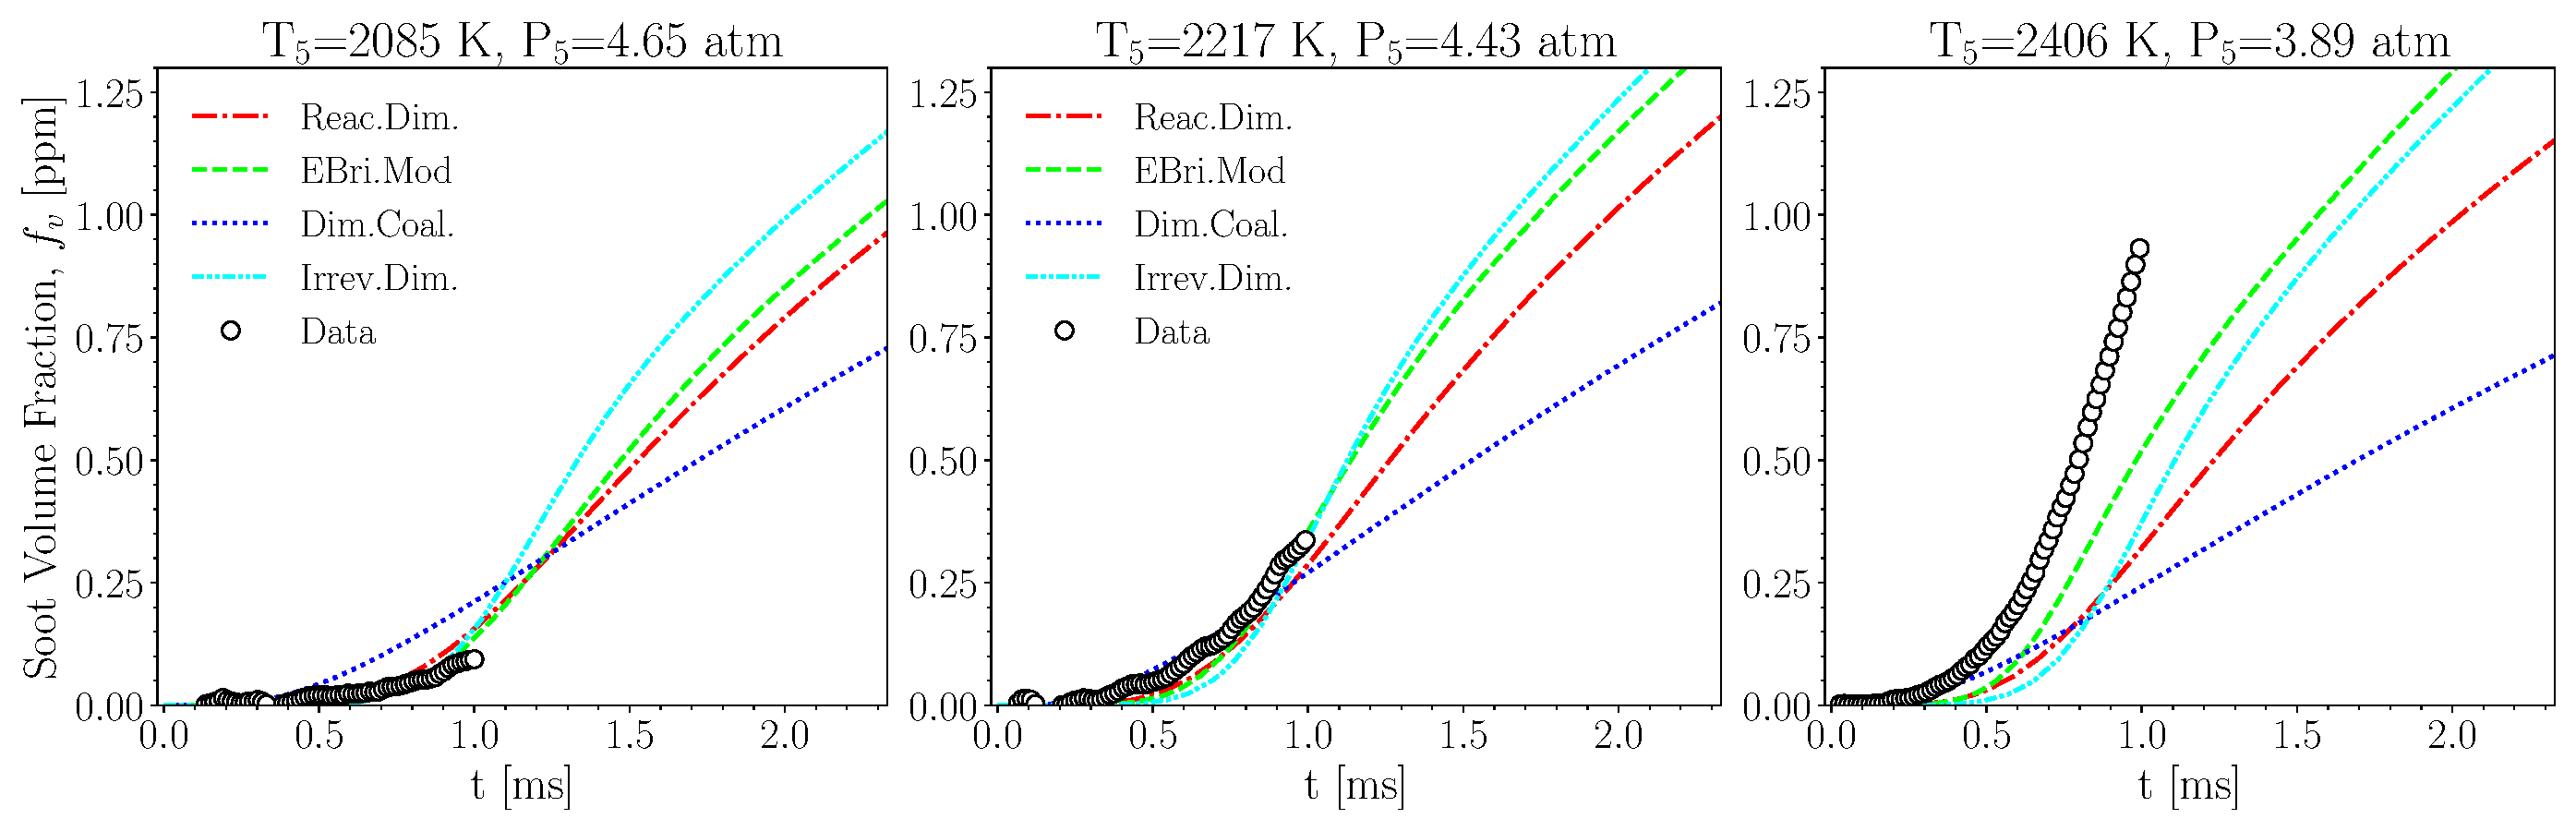
\includegraphics[width=1\textwidth]{Figures/Results/Shocktube/Stanford/September/10CH4_vf_pahopt_subset.pdf}
	\caption{The soot volume fraction, $f_v$ over 2000 K$<$T$<$2400 K, using KAUST, SPBM, and optimized inception models}
	\label{fig:shocktube_10_CH4_vf_incepopt} 
\end{figure}


\begin{figure}[H]
	\centering
	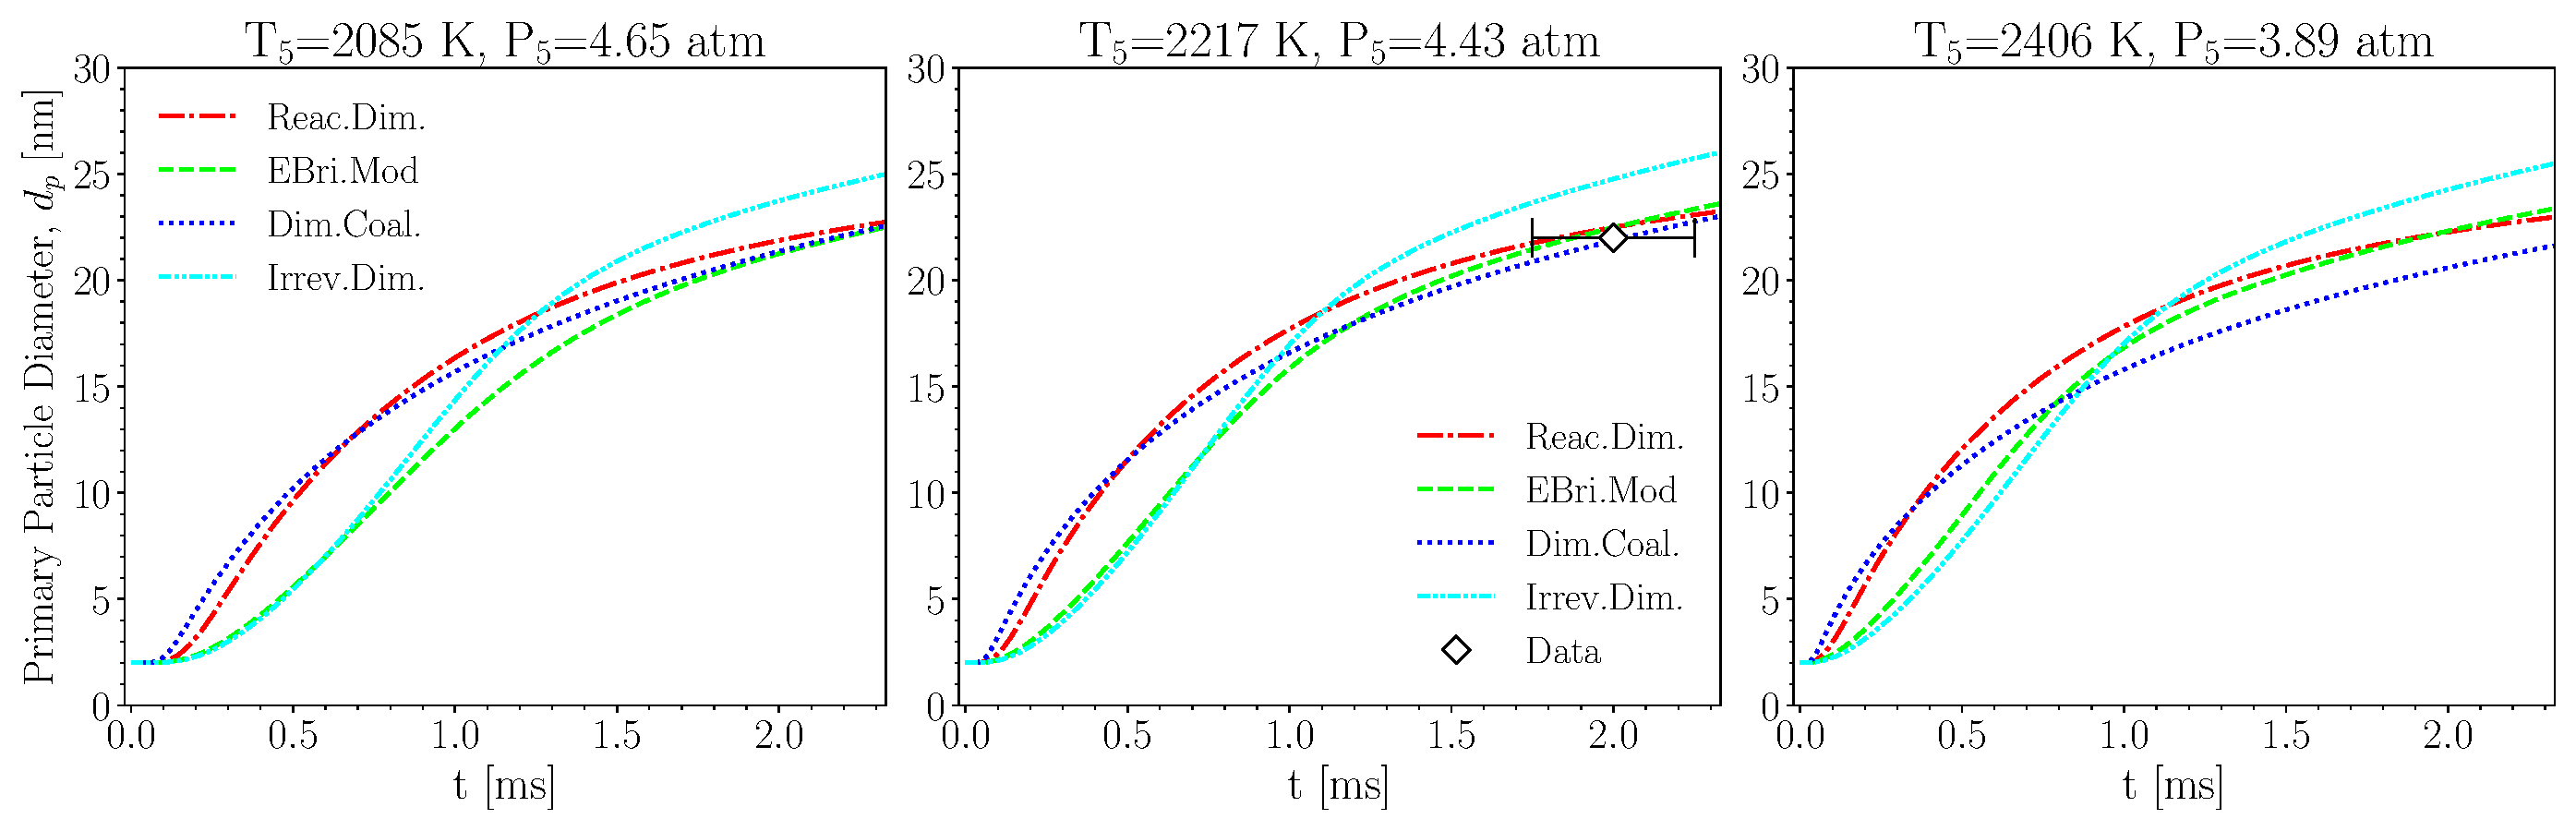
\includegraphics[width=1\textwidth]{Figures/Results/Shocktube/Stanford/September/10CH4_dp_pahopt_subset.pdf}
	\caption{The primary particle diameter, $d_p$ over 2000 K$<$T$<$2400 K, using KAUST, SPBM, and optimized inception models}
	\label{fig:shocktube_10_CH4_dp_incepopt} 
\end{figure}


\begin{figure}[H]
	\centering
	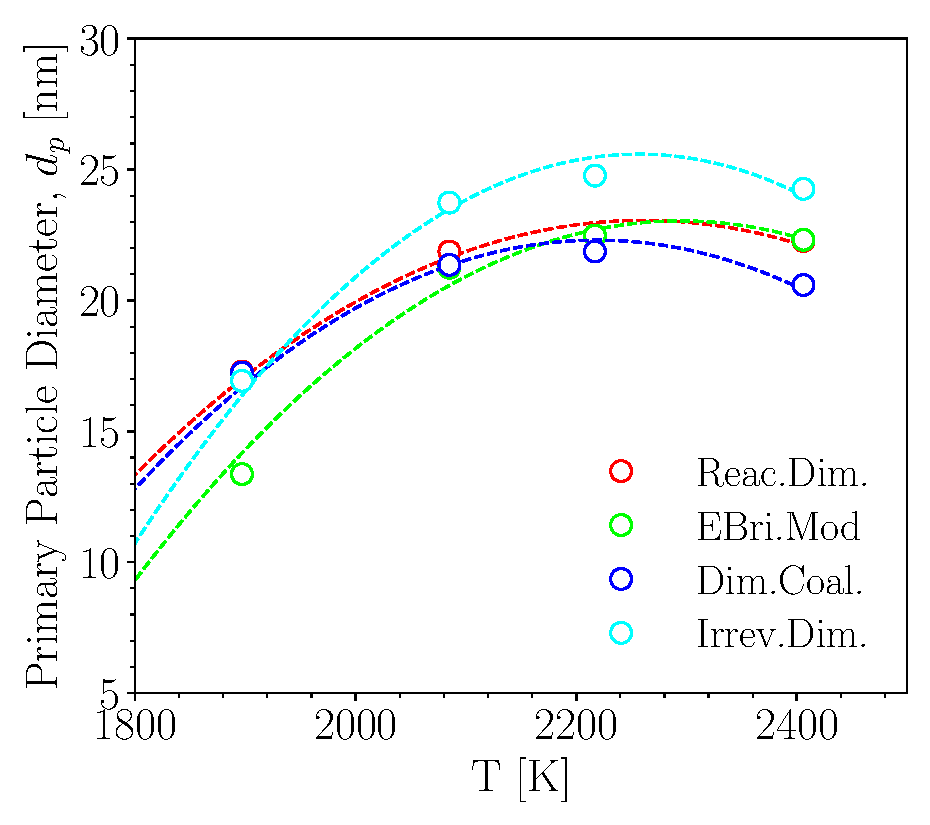
\includegraphics[width=0.32\textwidth]{Figures/Results/Shocktube/Stanford/September/10CH4_sootvf_kaust_2ms.pdf}
	\caption{The primary particle diameter, $d_p$ at t=2 ms over the studied temperature range using KAUST, SPBM, and optimized inception models. The dashed line is added to guide the eye.}
	\label{fig:shocktube_10_CH4_dp_incepopt_2ms} 
\end{figure}


